% \documentclass[aps,amssymb,amsmath,superscriptaddress,twocolumn,nofootinbib]{revtex4-1}
% \usepackage{hyperref}
% \usepackage{epsfig}
% \usepackage{bm}
% \usepackage{graphicx}
% \usepackage{epstopdf}
% \usepackage{physics}
% \usepackage{siunitx}
% \usepackage{colortbl}
% \usepackage[super]{nth}
% %\usepackage{rotate}
% %\usepackage{polyglossia}
% %\usepackage{unicode-math}
% \usepackage{color}
% %\usepackage{fontspec}
% \usepackage{subfigure}
% %\usepackage[affil-it]{authblk}
% %\usepackage{fixltx2e}
% %\usepackage{dblfloatfix}
% \usepackage{amsmath}
% \usepackage{mathtools}
% \hypersetup{
%     colorlinks=true,       % false: boxed links; true: colored links
%     linkcolor=cyan,          % color of internal links
%     citecolor=magenta,        % color of links to bibliography
%     filecolor=magenta,      % color of file links
%     urlcolor=cyan,           % color of external links
%     runcolor=cyan
% }
% \newcommand{\red}[1]{\textcolor{red}{#1}}
% \newcommand{\blue}[1]{\textcolor{blue}{#1}}
% \newcommand{\figurewidth}{0.8 \columnwidth}
% \newcommand{\beqarr}{\begin{eqnarray}}
% \newcommand{\eeqarr}{\end{eqnarray}}
% \newcommand{\beq}{\begin{equation}}
% \newcommand{\eeq}{\end{equation}}
% \newcommand{\e}{{\text e}}
% \newcommand{\rmd}{{\text d}}
% \newcommand{\mc}{\mathcal}
% \newcommand{\JJ}[1]{{\textcolor{red}{[#1]}}}
% \newcommand{\DL}[1]{{\textcolor{blue}{[#1]}}}
% \newcommand{\GeV}{\giga\electronvolt}
% \newcommand{\TeV}{\tera\electronvolt}
% \newcommand{\ignore}[1]{}
% \newtheorem{dictum}{Dictum}
%
% \keywords{quantum annealing, quantum computing, benchmarking, validation, error correction}
%
% \usepackage[printwatermark]{xwatermark}
% \usepackage{xcolor}
% \usepackage{graphicx}
% \usepackage{lipsum}
%
% \begin{document}



% \author{Joshua Job}
% \affiliation{Department of Physics and Astronomy, University of Southern California, Los Angeles, California 90089, USA}
% \affiliation{Center for Quantum Information Science \& Technology, University of Southern California, Los Angeles, California 90089, USA}
%
% \author{Daniel Lidar}
% \affiliation{Department of Physics and Astronomy, University of Southern California, Los Angeles, California 90089, USA}
% \affiliation{Center for Quantum Information Science \& Technology, University of Southern California, Los Angeles, California 90089, USA}
% \affiliation{Department of Electrical Engineering, University of Southern California, Los Angeles, California 90089, USA}
% \affiliation{Department of Chemistry, University of Southern California, Los Angeles, California 90089, USA}







% Once one has validated that the device works in approximately the manner one would expect from the instruction manual, one can then turn to the question: ``Toward what practical purpose may this device be put?". The choice of appropriate problems in this domain is a complex issue that we cannot address here. Indeed, before we can answer that question, we must first focus on an operational question: ``How does one go about comparing performance in a specified problem domain between a verified quantum computing device and existing classical strategies?". We discuss this next.

\section{Benchmarking}
\label{section:benchmarking}



\subsection{The state of benchmarking}



%The main focus of Ref.~\cite{q108} was in fact not benchmarking, but quantum validation testing, as described in Sec.~\ref{sec:QVT-expt}.



\subsection{Lessons}
What lessons may be gleaned from this story for future benchmarks of quantum annealing devices with limited or no error correction and hundreds or thousands of qubits?
\begin{enumerate}
	\item It is vitally important to carefully account for resource use, lest one be led astray with a fake speedup. In particular, quantum annealing requires a demonstration of an optimal annealing time before any definitive conclusion can be drawn about a quantum speedup. More generally, optimizing all known free parameters is almost certainly necessary to demonstrate a quantum speedup which will hold up to scrutiny.
	\item One must distinguish between different types of quantum speedup. Comparisons between a quantum computational device and a single other solver are inherently limited to a demonstration of a ``potential quantum speedup". To go further, one must be sure to compare performance against a suite of algorithms, in particular those that mimic the device to some degree (such as SA or SQA). A speedup against such solvers would be considered a ``limited quantum speedup". If there is a consensus about the solvers that are the best at the original task, then a speedup against such solvers would be considered an unqualified ``quantum speedup". This would be a game-changing result.
	\item Users of such quantum computational devices should perform something akin to gauge averaging in order to effectively estimate performance, by averaging over many different mappings from the logical problem to physical states, at least so long as the devices are not fully error corrected. Given that there is no good distribution for problem hardness as a function of this ensemble of mappings, nonparameteric techniques are appropriate.\footnote{We suggest using a variant of the bootstrap, the Bayesian bootstrap, first introduced in Ref.~\cite{rubin1981bayesian}, which can be shown to be the limit in the case of negligible prior information or large amounts of data of a Dirichlet process. Thus, it is arguably the only bootstrap procedure which is well-founded on Bayesian grounds. It involves reweighting the observed data, much like every bootstrap, but rather than sampling from a Multinomial$(N,[1/N,\ldots,1/N])$ distribution as in the frequentist bootstrap, one instead samples from the related Dirichlet$(1,\ldots,1)$ distribution. The primary advantage of the Bayesian bootstrap is that, unlike the frequentist bootstrap, the weight assigned any element in the dataset is always positive, i.e., there are no reweighted data vectors which leave out a data element, whereas the frequentist bootstrap has probability $1/e$ of dropping any given data element in a reweighted sample.}
	\item Choice of benchmark problem is key, and should be made with an eye toward the day when classical machines are vastly outpaced by quantum devices. For example, the transition from random Ising problems to frustrated loop/planted solutions problems was forced by the need to have reasonable benchmarks for devices so large that classical systems cannot solve them in a human lifetime.
\end{enumerate}

So far we have only addressed the question of benchmarking without any attempt at error correction. Since it is impossible to achieve a scalable quantum speedup without some means of correcting for errors, while benchmarking native problems may give some indication of the abilities of quantum annealing by looking at relatively small problem sizes, work on error correction lays the foundation for potential lasting quantum advantages over classical computing.



\begin{figure}[t]
\begin{center}
\subfloat[]{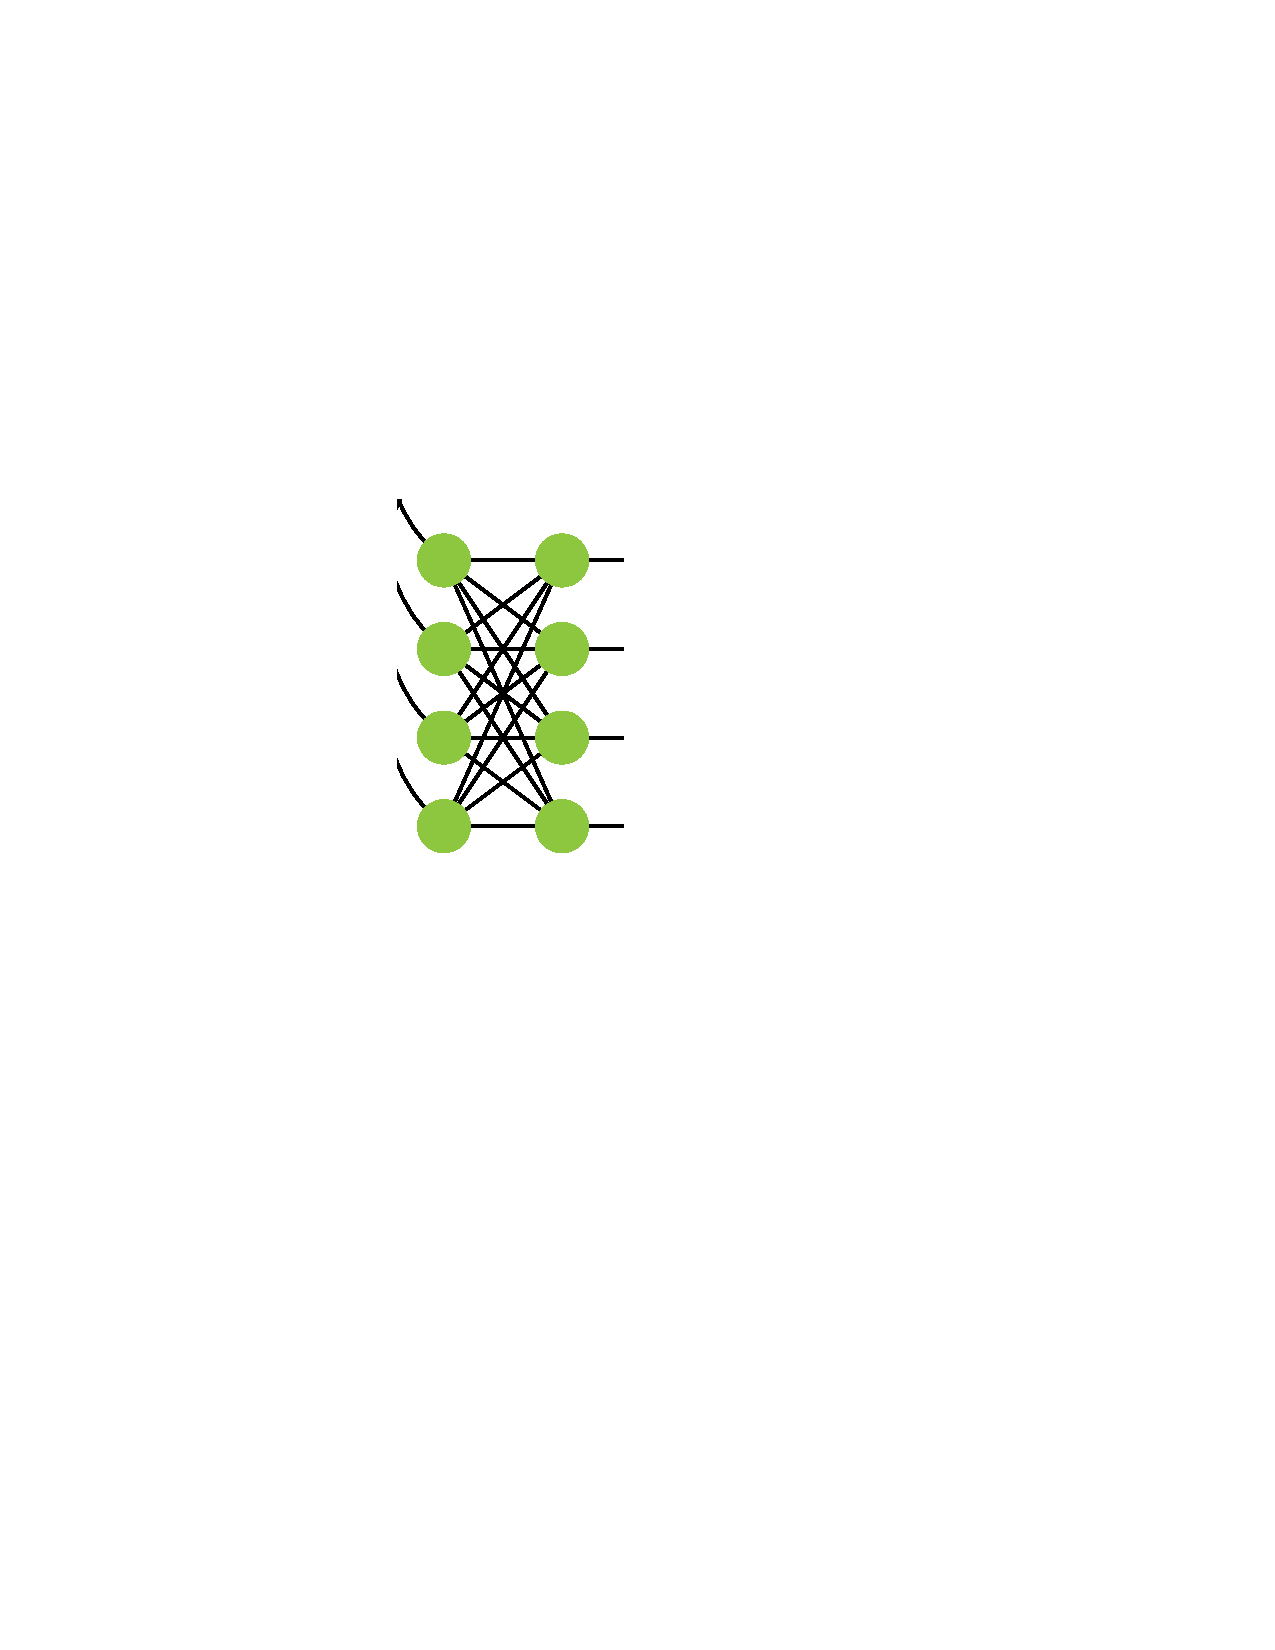
\includegraphics[width=0.12\textwidth]{chapters/Test-driving/unitcell}\label{fig:unitcell}}\\
\subfloat[]{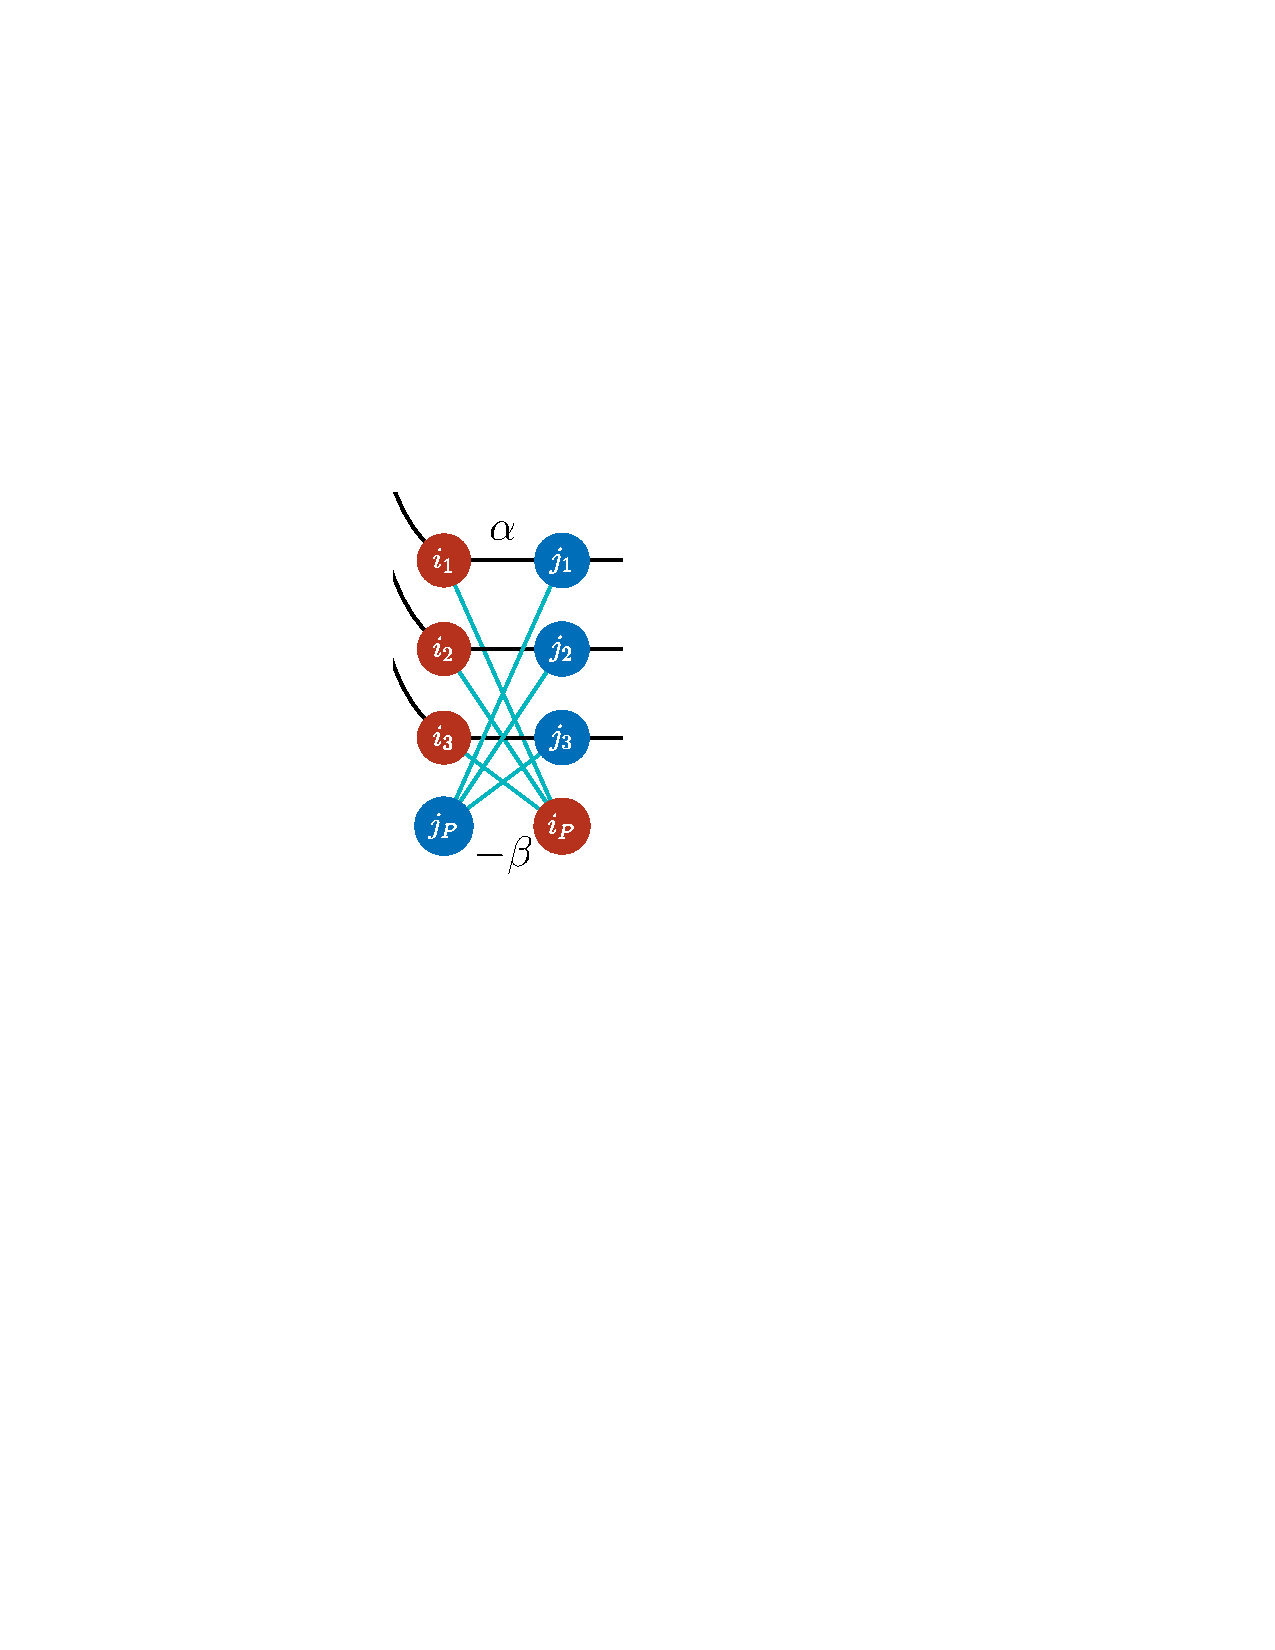
\includegraphics[width=0.12\textwidth]{chapters/Test-driving/QACencoding}\label{fig:QACencoding}}\\
\subfloat[]{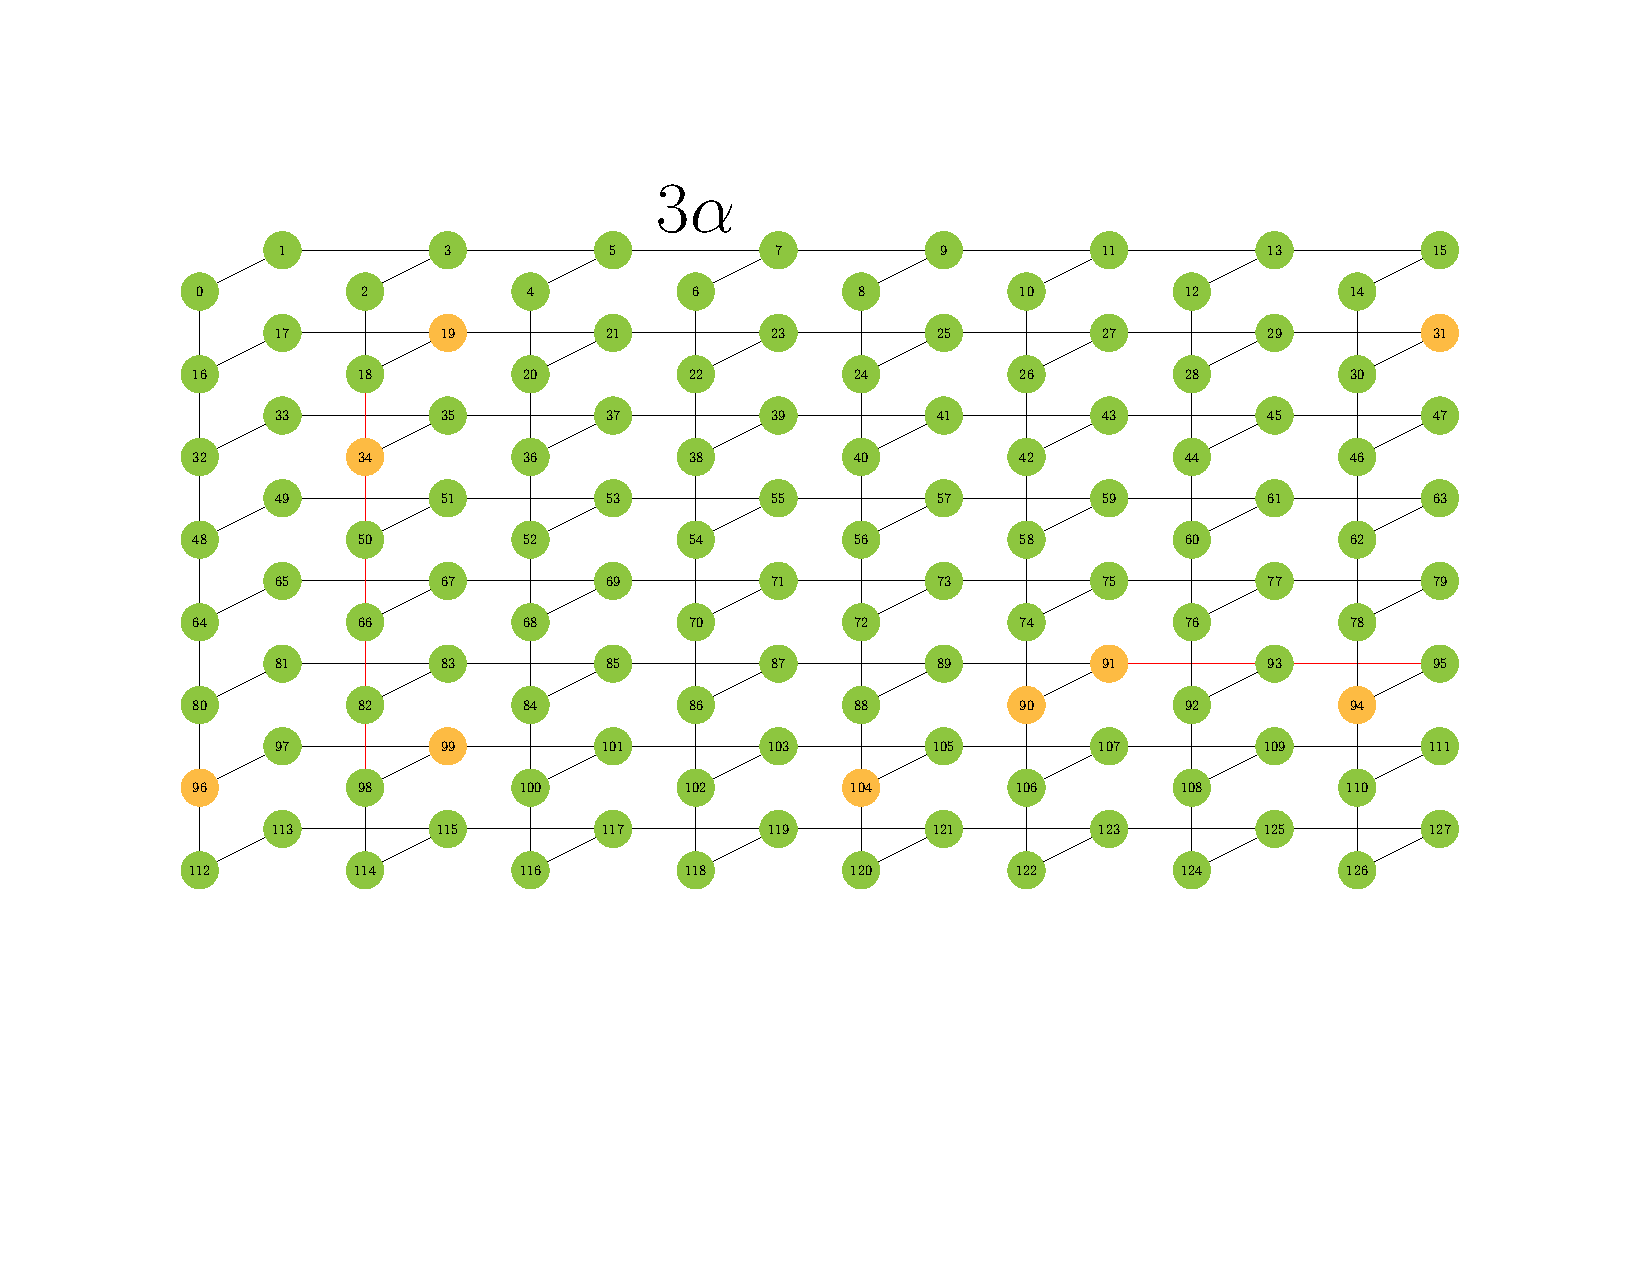
\includegraphics[width=0.48\textwidth]{chapters/Test-driving/QACencodedHamiltonian}\label{fig:QACencodedHamiltonian}}
\end{center}
\caption{The QAC unit cell and encoded graph introduced in Refs.~\cite{PAL:13,PAL:14}. (a) Schematic of one of the $64$ {unit cells} of the DW2 processor. Unit cells are arranged in an $8\times 8$ array forming a ``Chimera" graph between qubits. Each circle represents a physical qubit, and each line a programmable Ising coupling $\sigma^z_i\sigma^z_j$. Lines on the right (left) couple to the corresponding qubits in the neighboring unit cell to the right (above).
(b) Two ``logical qubits" ($i$, red and $j$, blue) embedded within a single unit cell. Qubits labeled 1-3 are the ``problem qubits", the opposing qubit of the same color labeled $P$ is the ``penalty qubit". Problem qubits couple via the black lines with tunable strength $\alpha$ both inter- and intra-unit cell. Light blue lines of magnitude $\beta$ are ferromagnetic couplings between the problem qubits and their penalty qubit. (c) Encoded processor graph obtained from the Chimera graph by replacing each logical qubit by a circle. This is a non-planar graph with couplings of strength $3\alpha$. Green circles represent  complete logical qubits. Orange circles represent logical qubits lacking their penalty qubit. Red lines are {groups of} couplers that cannot {all} be simultaneously activated.
}
\label{fig:QAC}
\end{figure}

%%%%%%
\begin{figure*}[ht]
\begin{center}
\subfloat[\ 2LG logical graph connectivity]{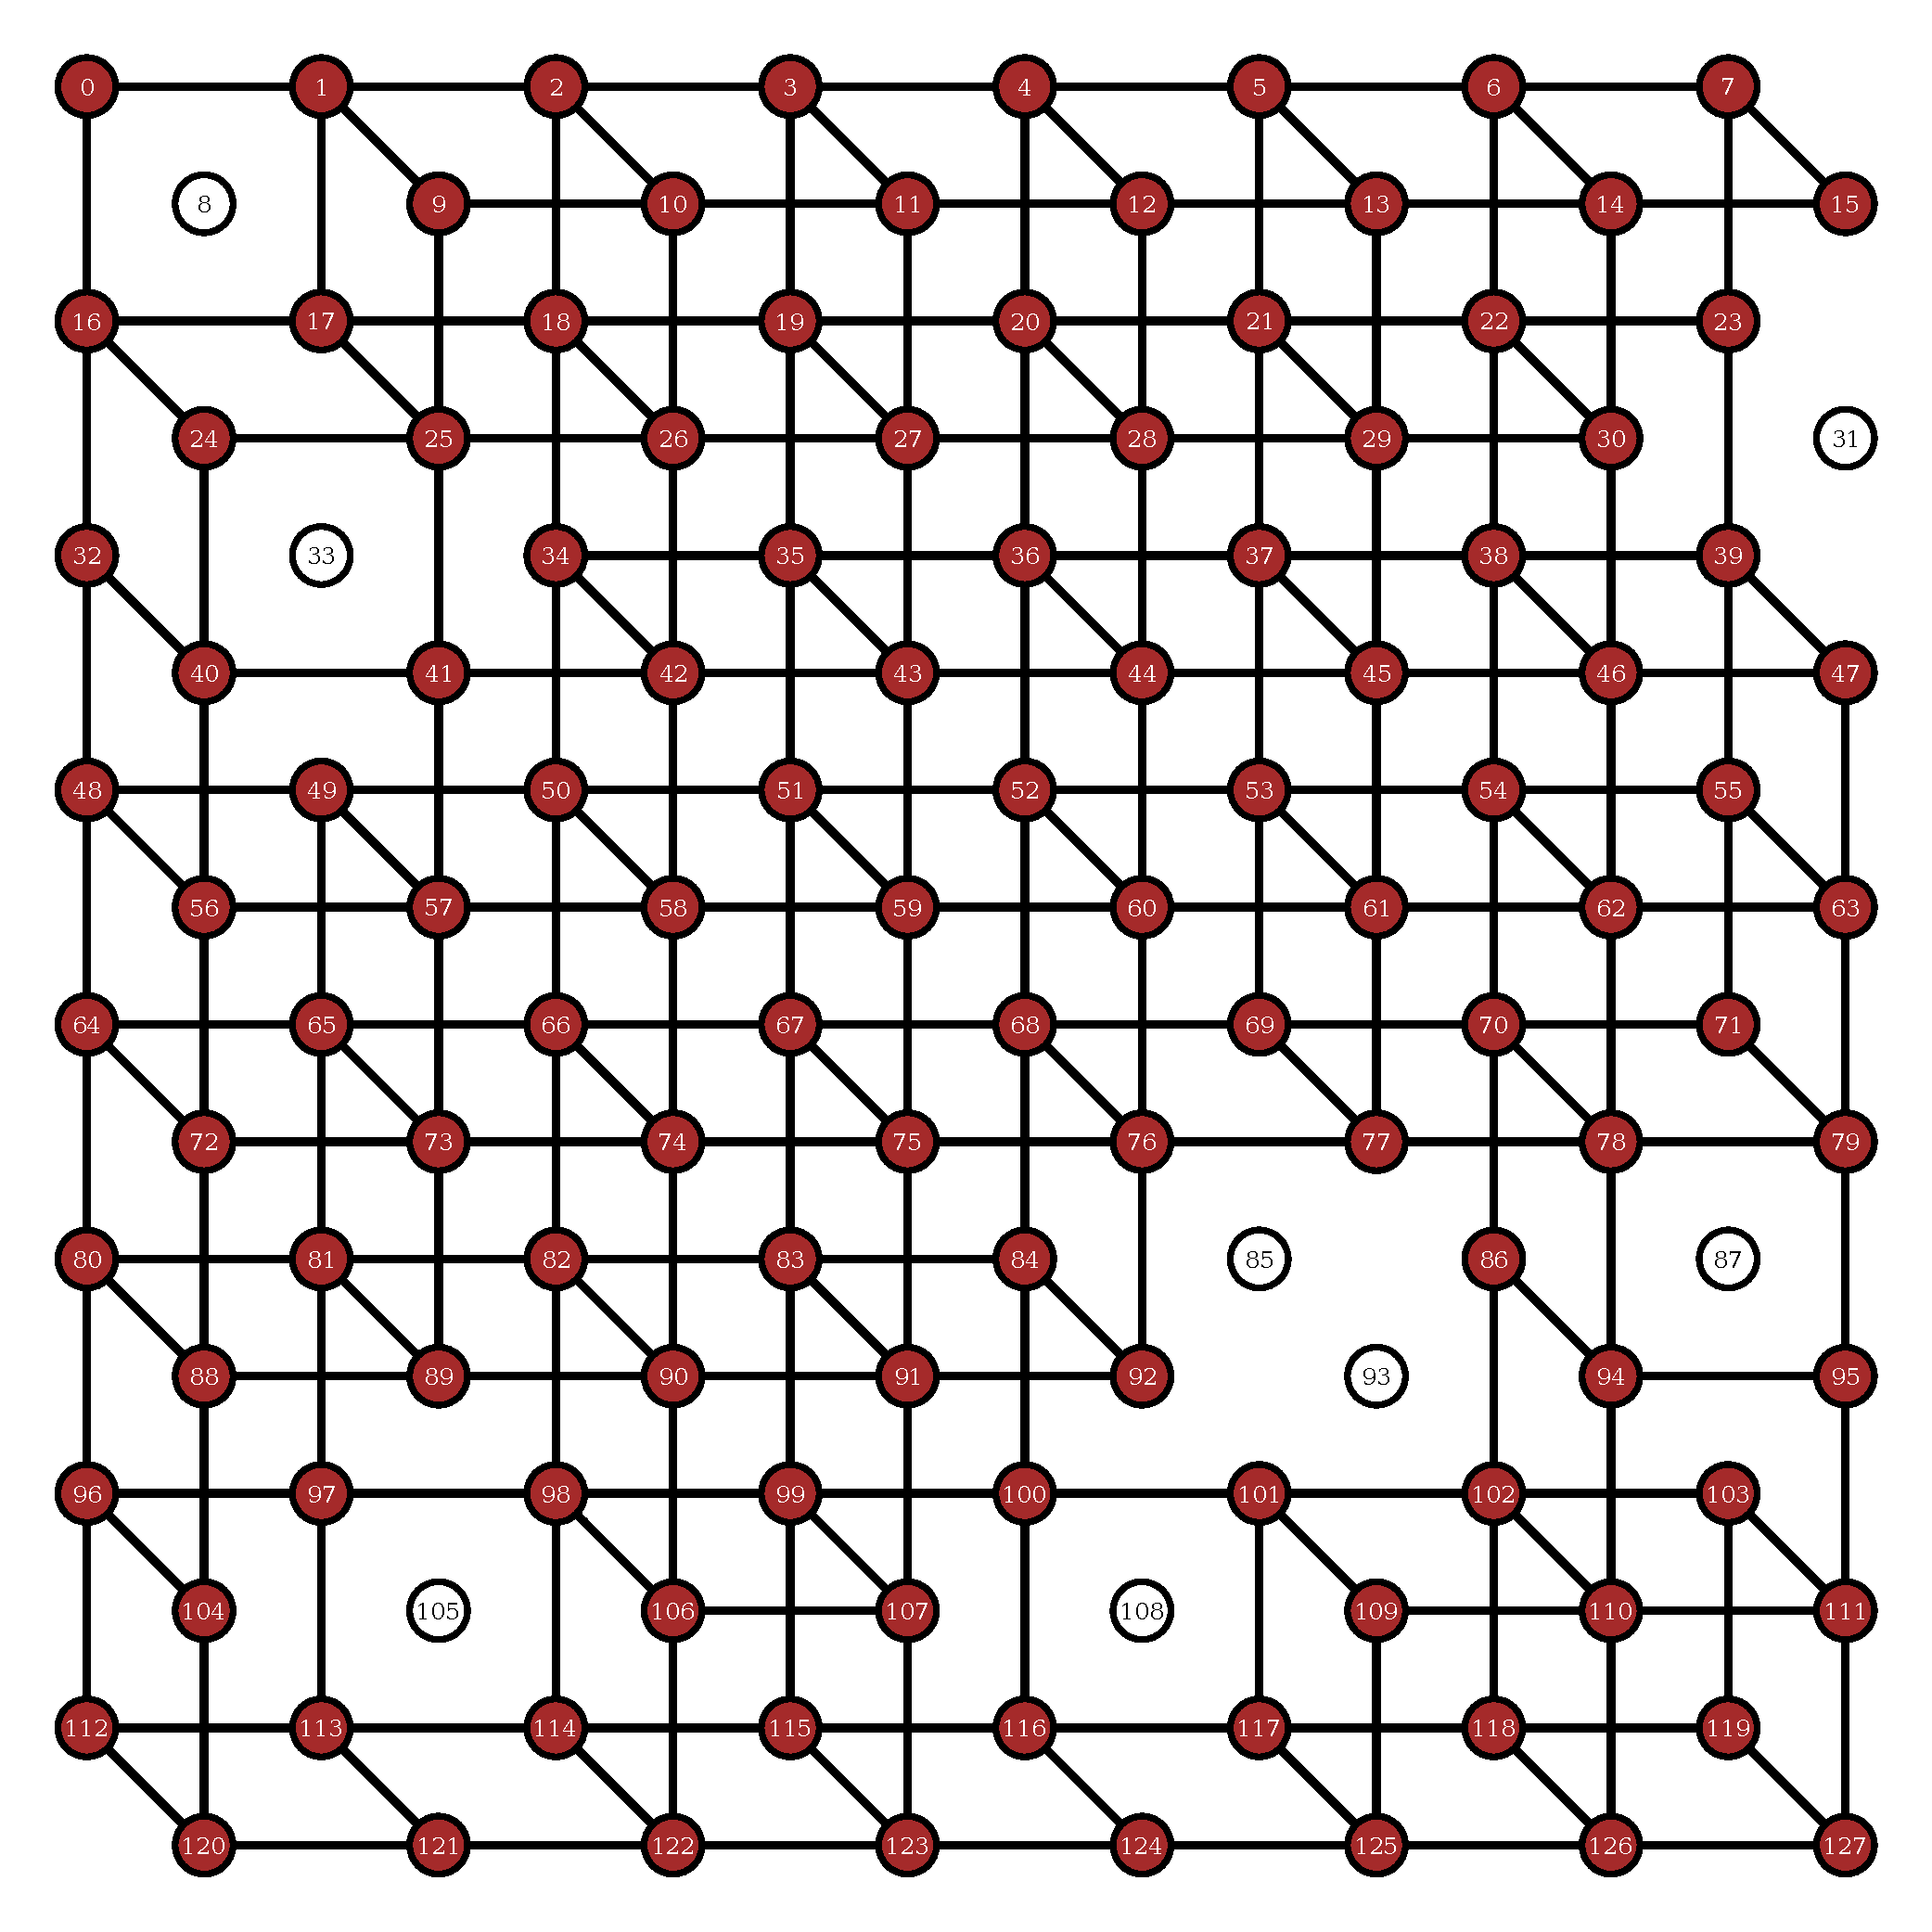
\includegraphics[width=0.32\textwidth]{chapters/Test-driving/VesuviusLogical}\label{fig:square-code-a}}
\subfloat[\ Minor embedding into Chimera graph]{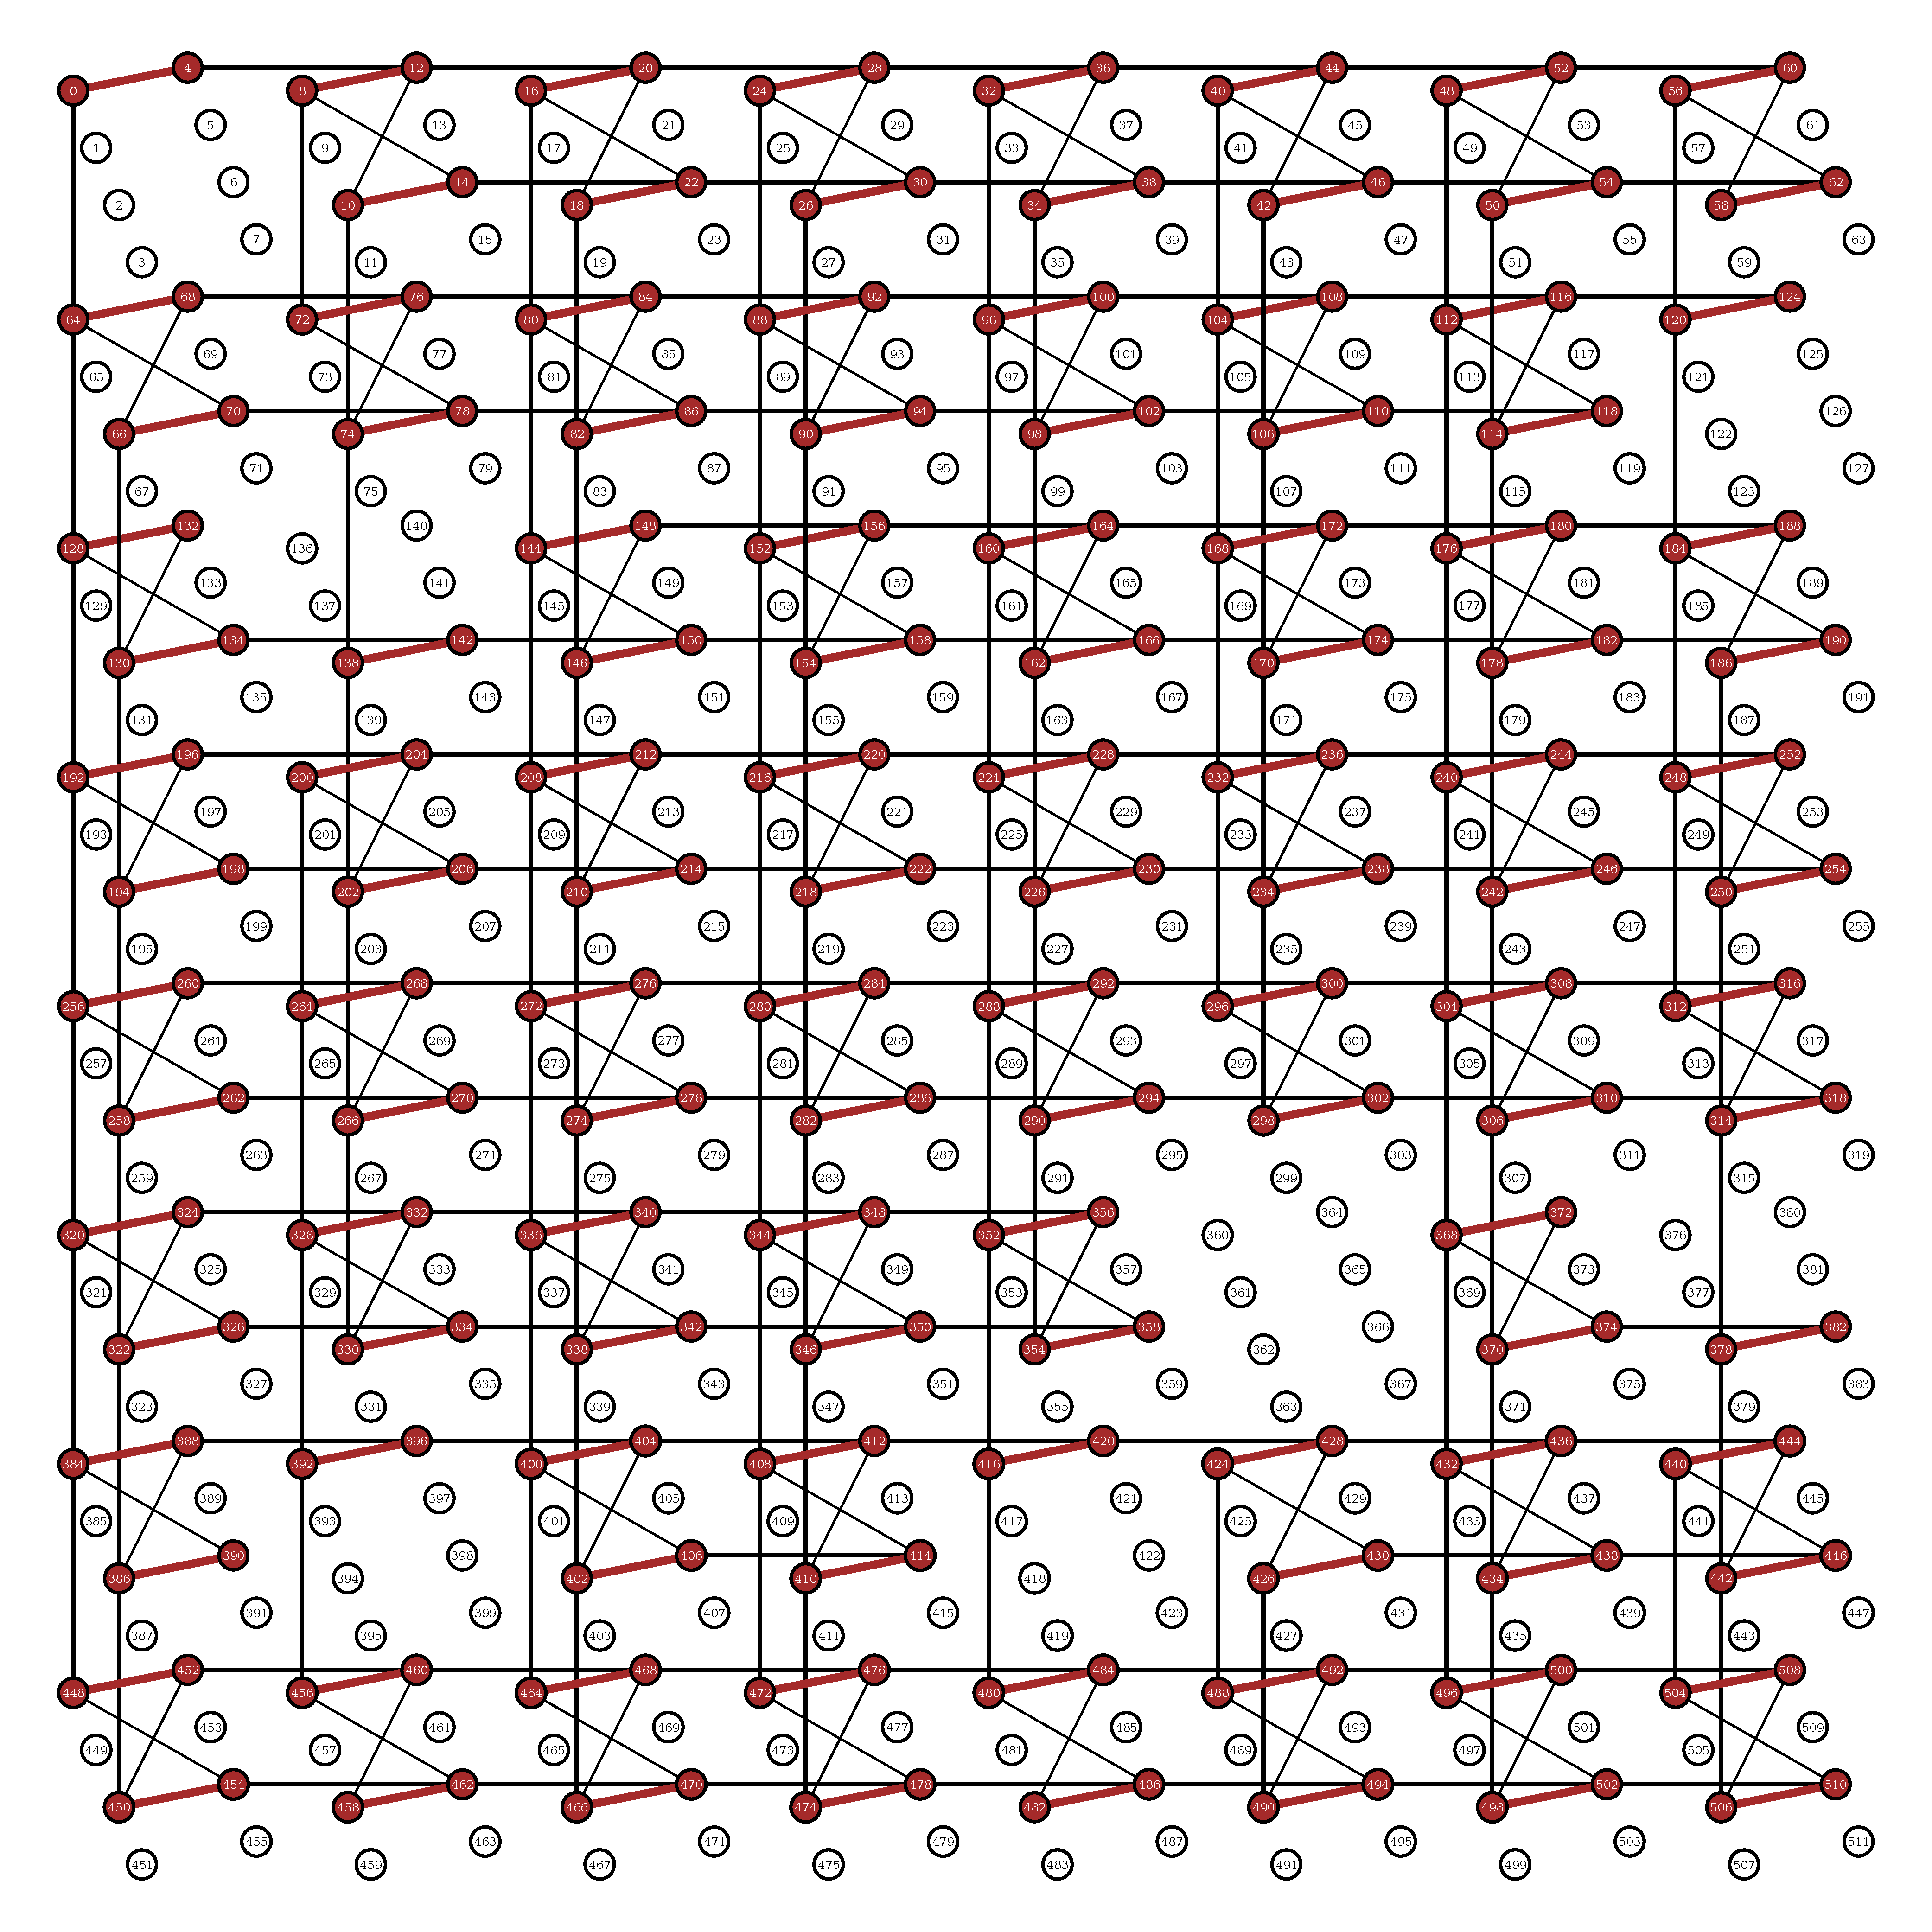
\includegraphics[width=0.32\textwidth]{chapters/Test-driving/ColoringMask_ME}\label{fig:square-code-b}}
\subfloat[\ QAC-ME]{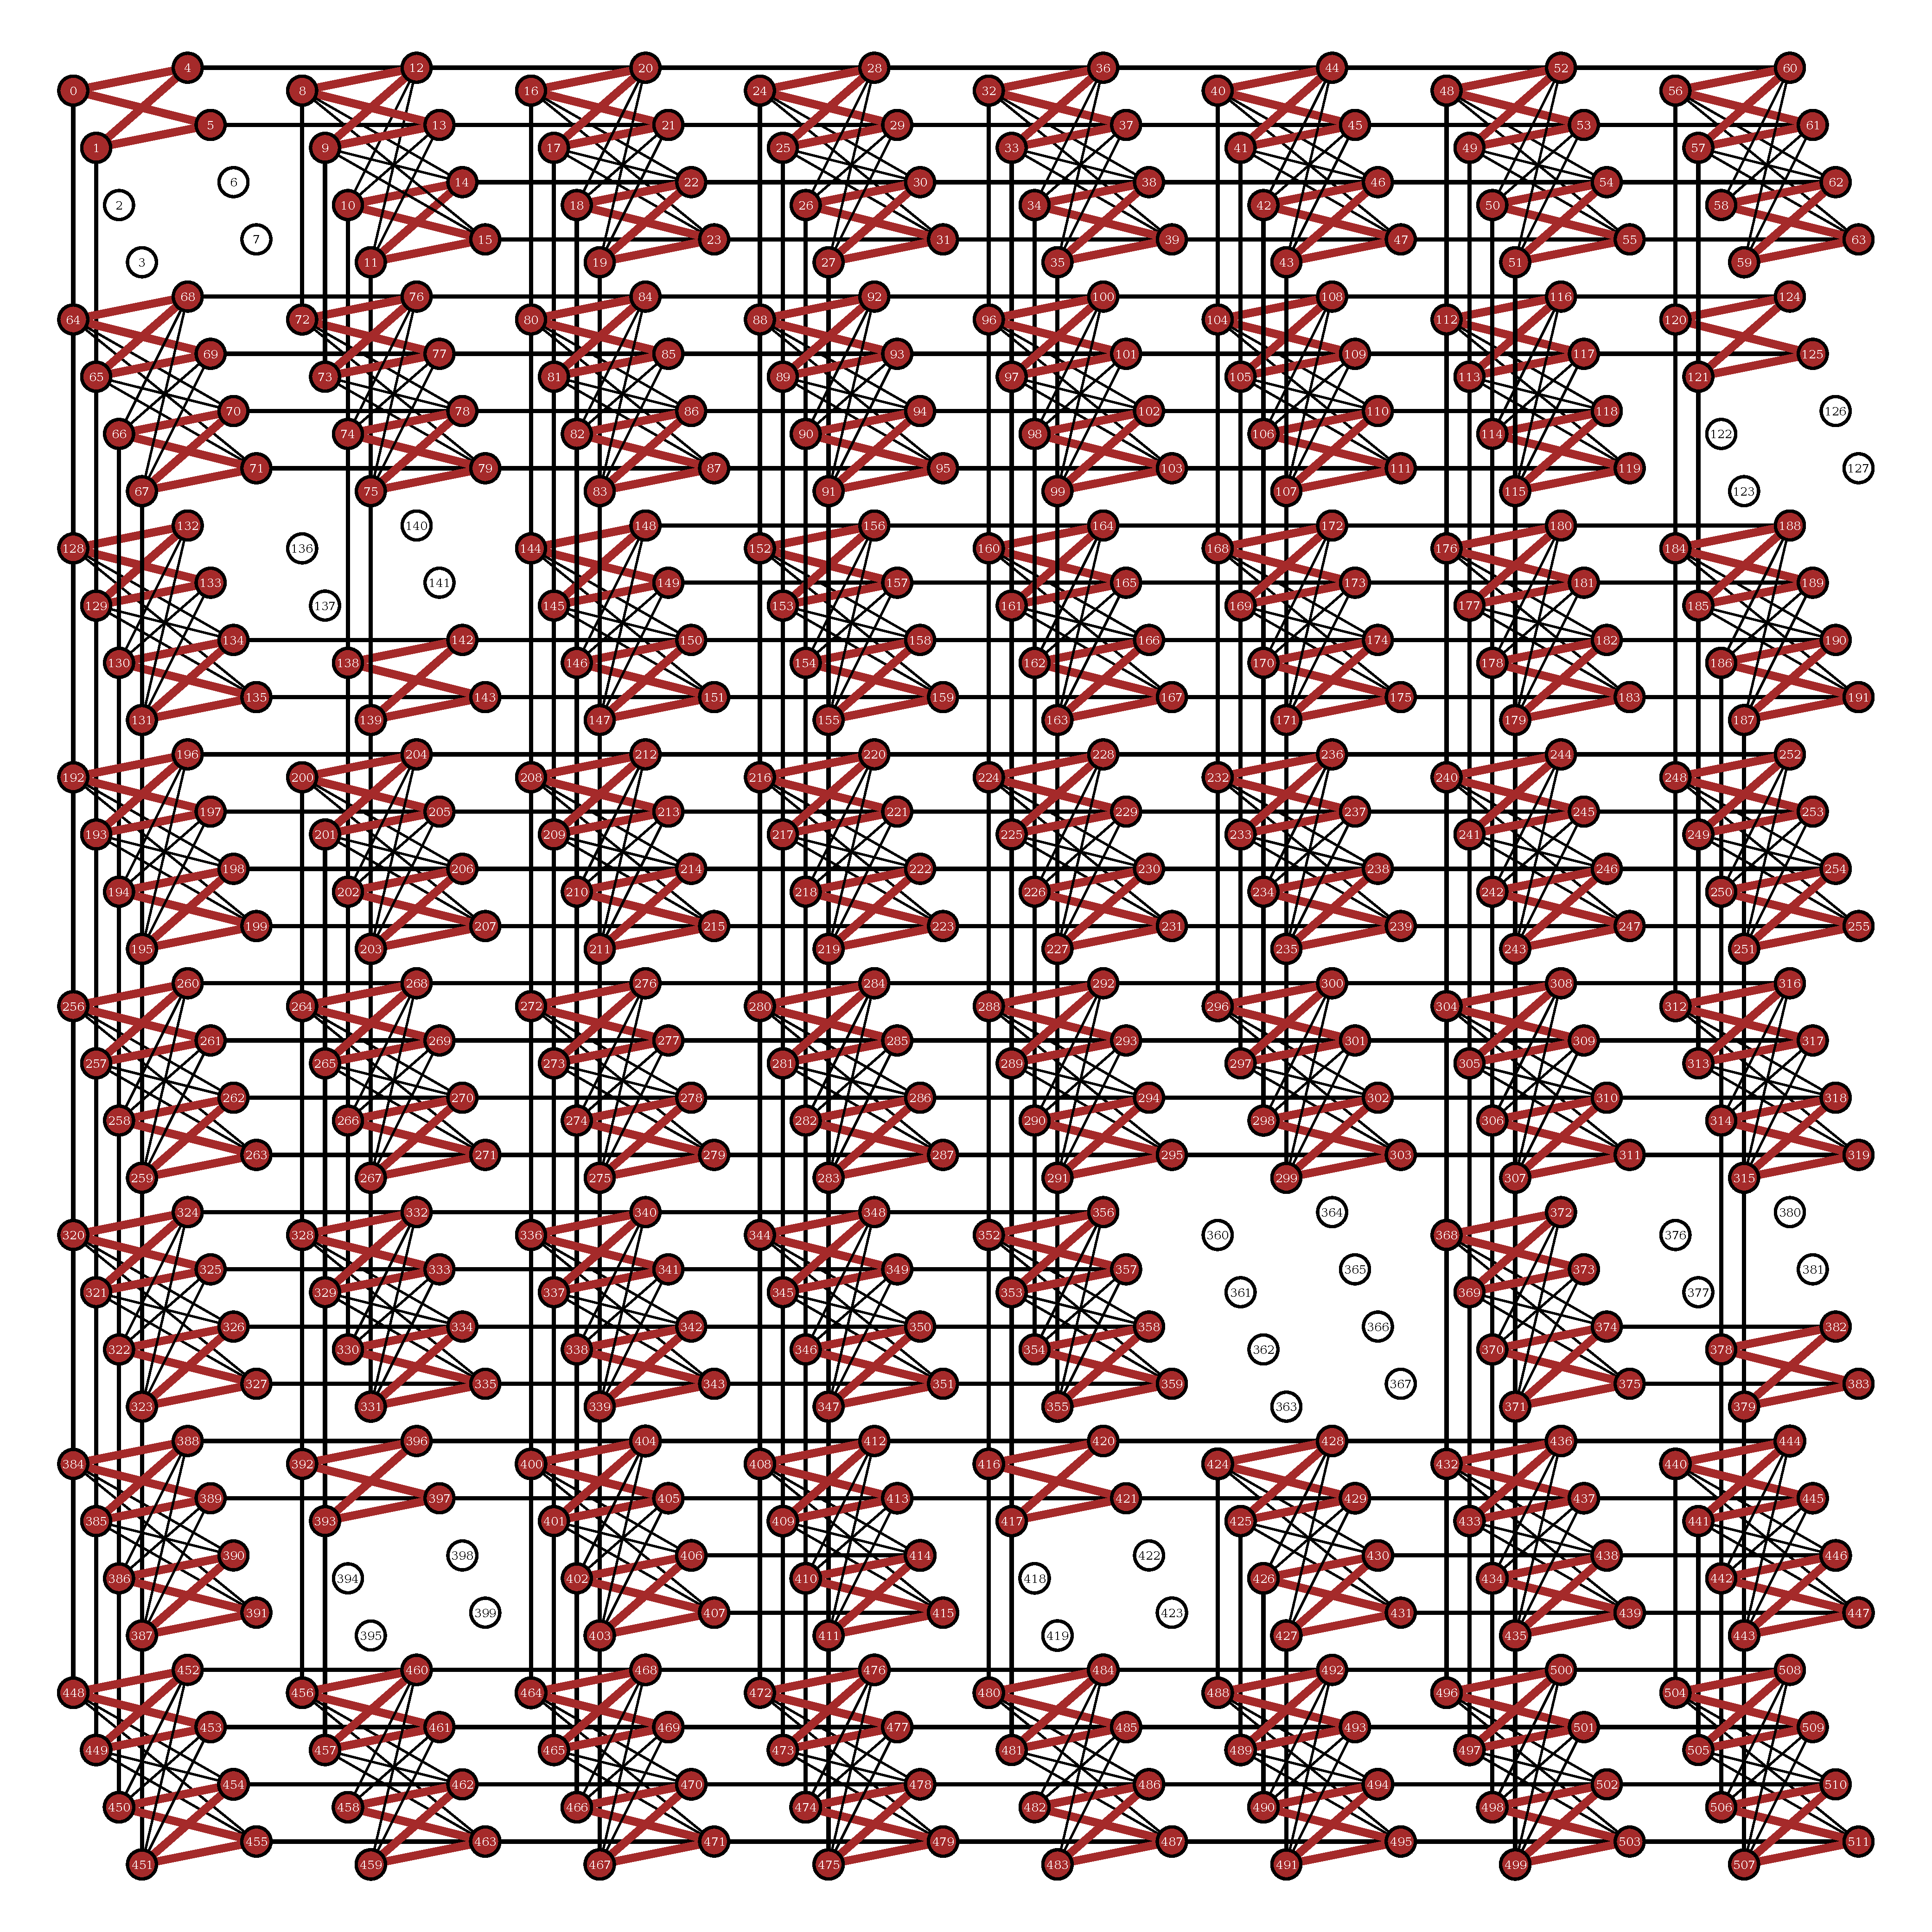
\includegraphics[width=0.32\textwidth]{chapters/Test-driving/ColoringMask_QEC}\label{fig:square-code-c}}
\caption{Illustration of mapping from a logical problem to a QAC-ME embedding, introduced in Ref.~\cite{Vinci:2015jt}. (a) The two-level-grid (2LG) graph, for which the Ising spin glass problem with couplings in $\{-1,0,1\}$ is NP-hard \cite{Barahona1982}. Disconnected vertices indicate spins with couplings set to zero, as well as  unused logical qubits in the logical DW2 Chimera graph. (b) Minor embedding of the 2LG graph into the physical DW2 Chimera graph. White circles correspond to unused or unusable qubits. (c) QAC-ME embedding of the 2LG problem using the ``square'' code.
In (b) and (c) penalties are represented by red (thick) couplings between groups of two (ME) and four (QAC-ME) physical qubits. Black (thin) links implement logical couplings.}
\label{fig:square-code}
\end{center}
\end{figure*}
%%%%%%

\begin{figure}[t]
\begin{center}
\subfloat[\ Logical graph: 1st level.]{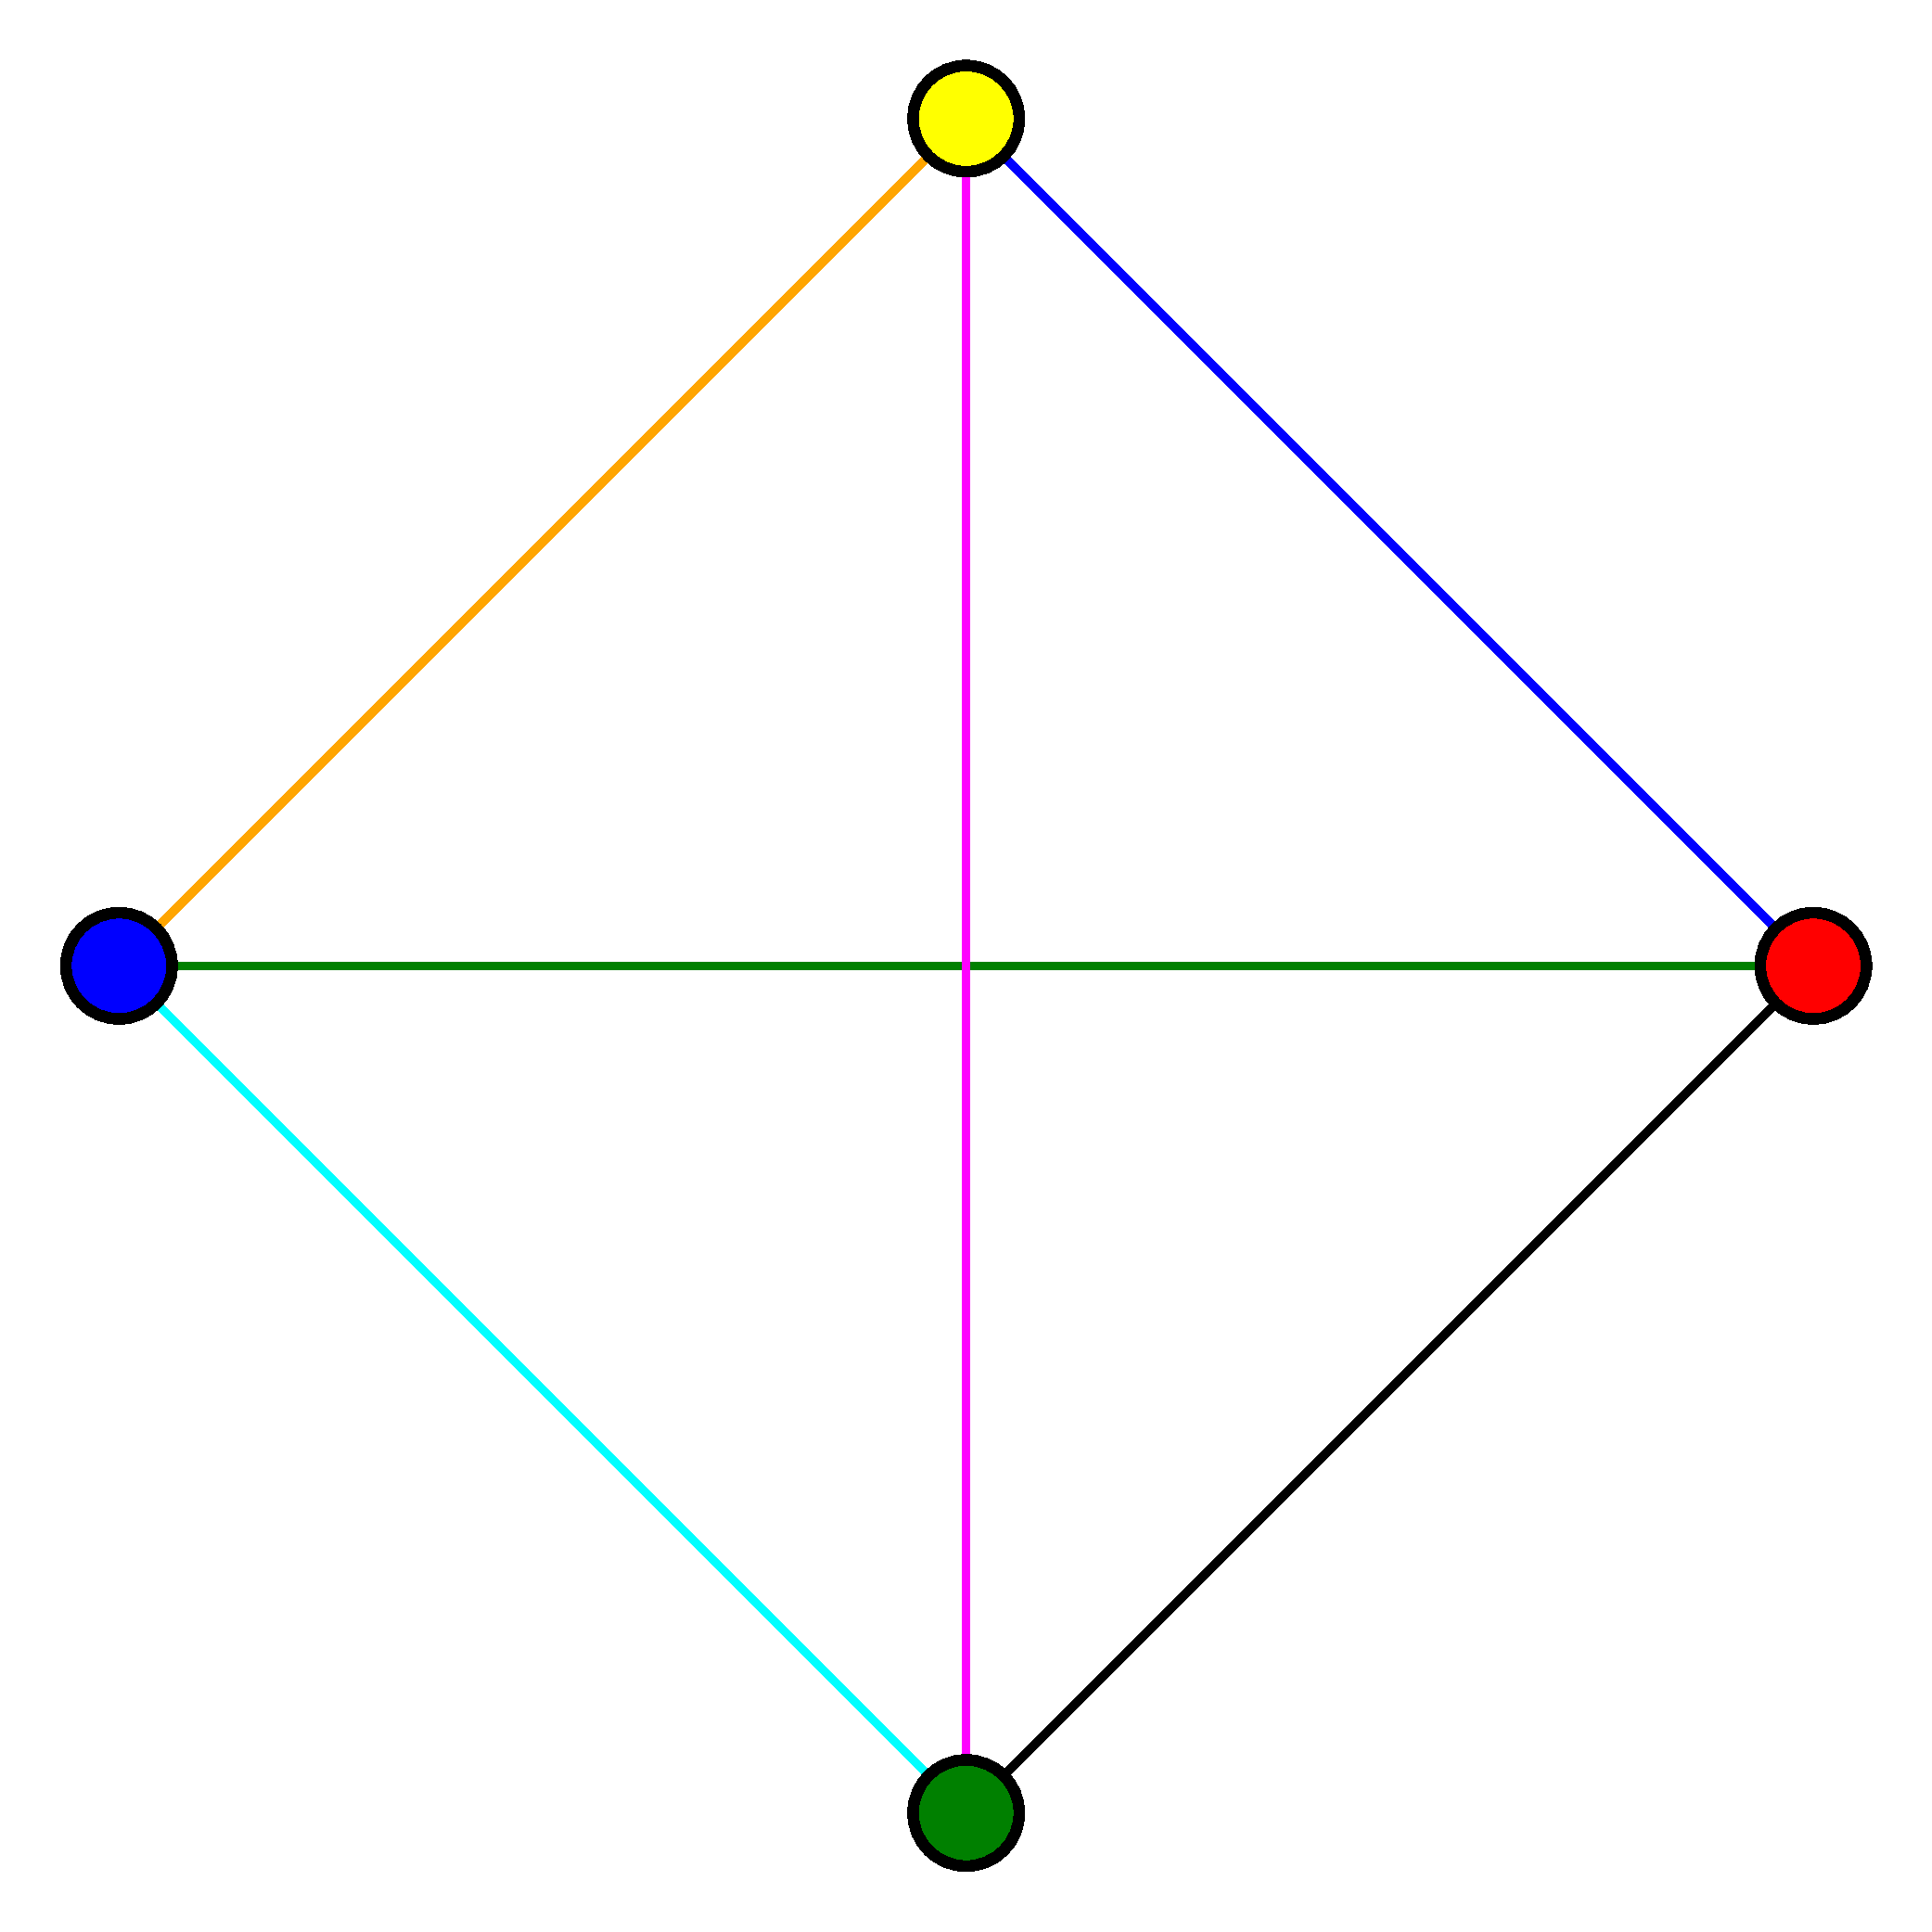
\includegraphics[width=0.23\textwidth]{chapters/Test-driving/4x4_ideal_logical_plot_1}\label{fig:4x4_ideal_logical_plot_1}}
\subfloat[\ 1st level ME.]{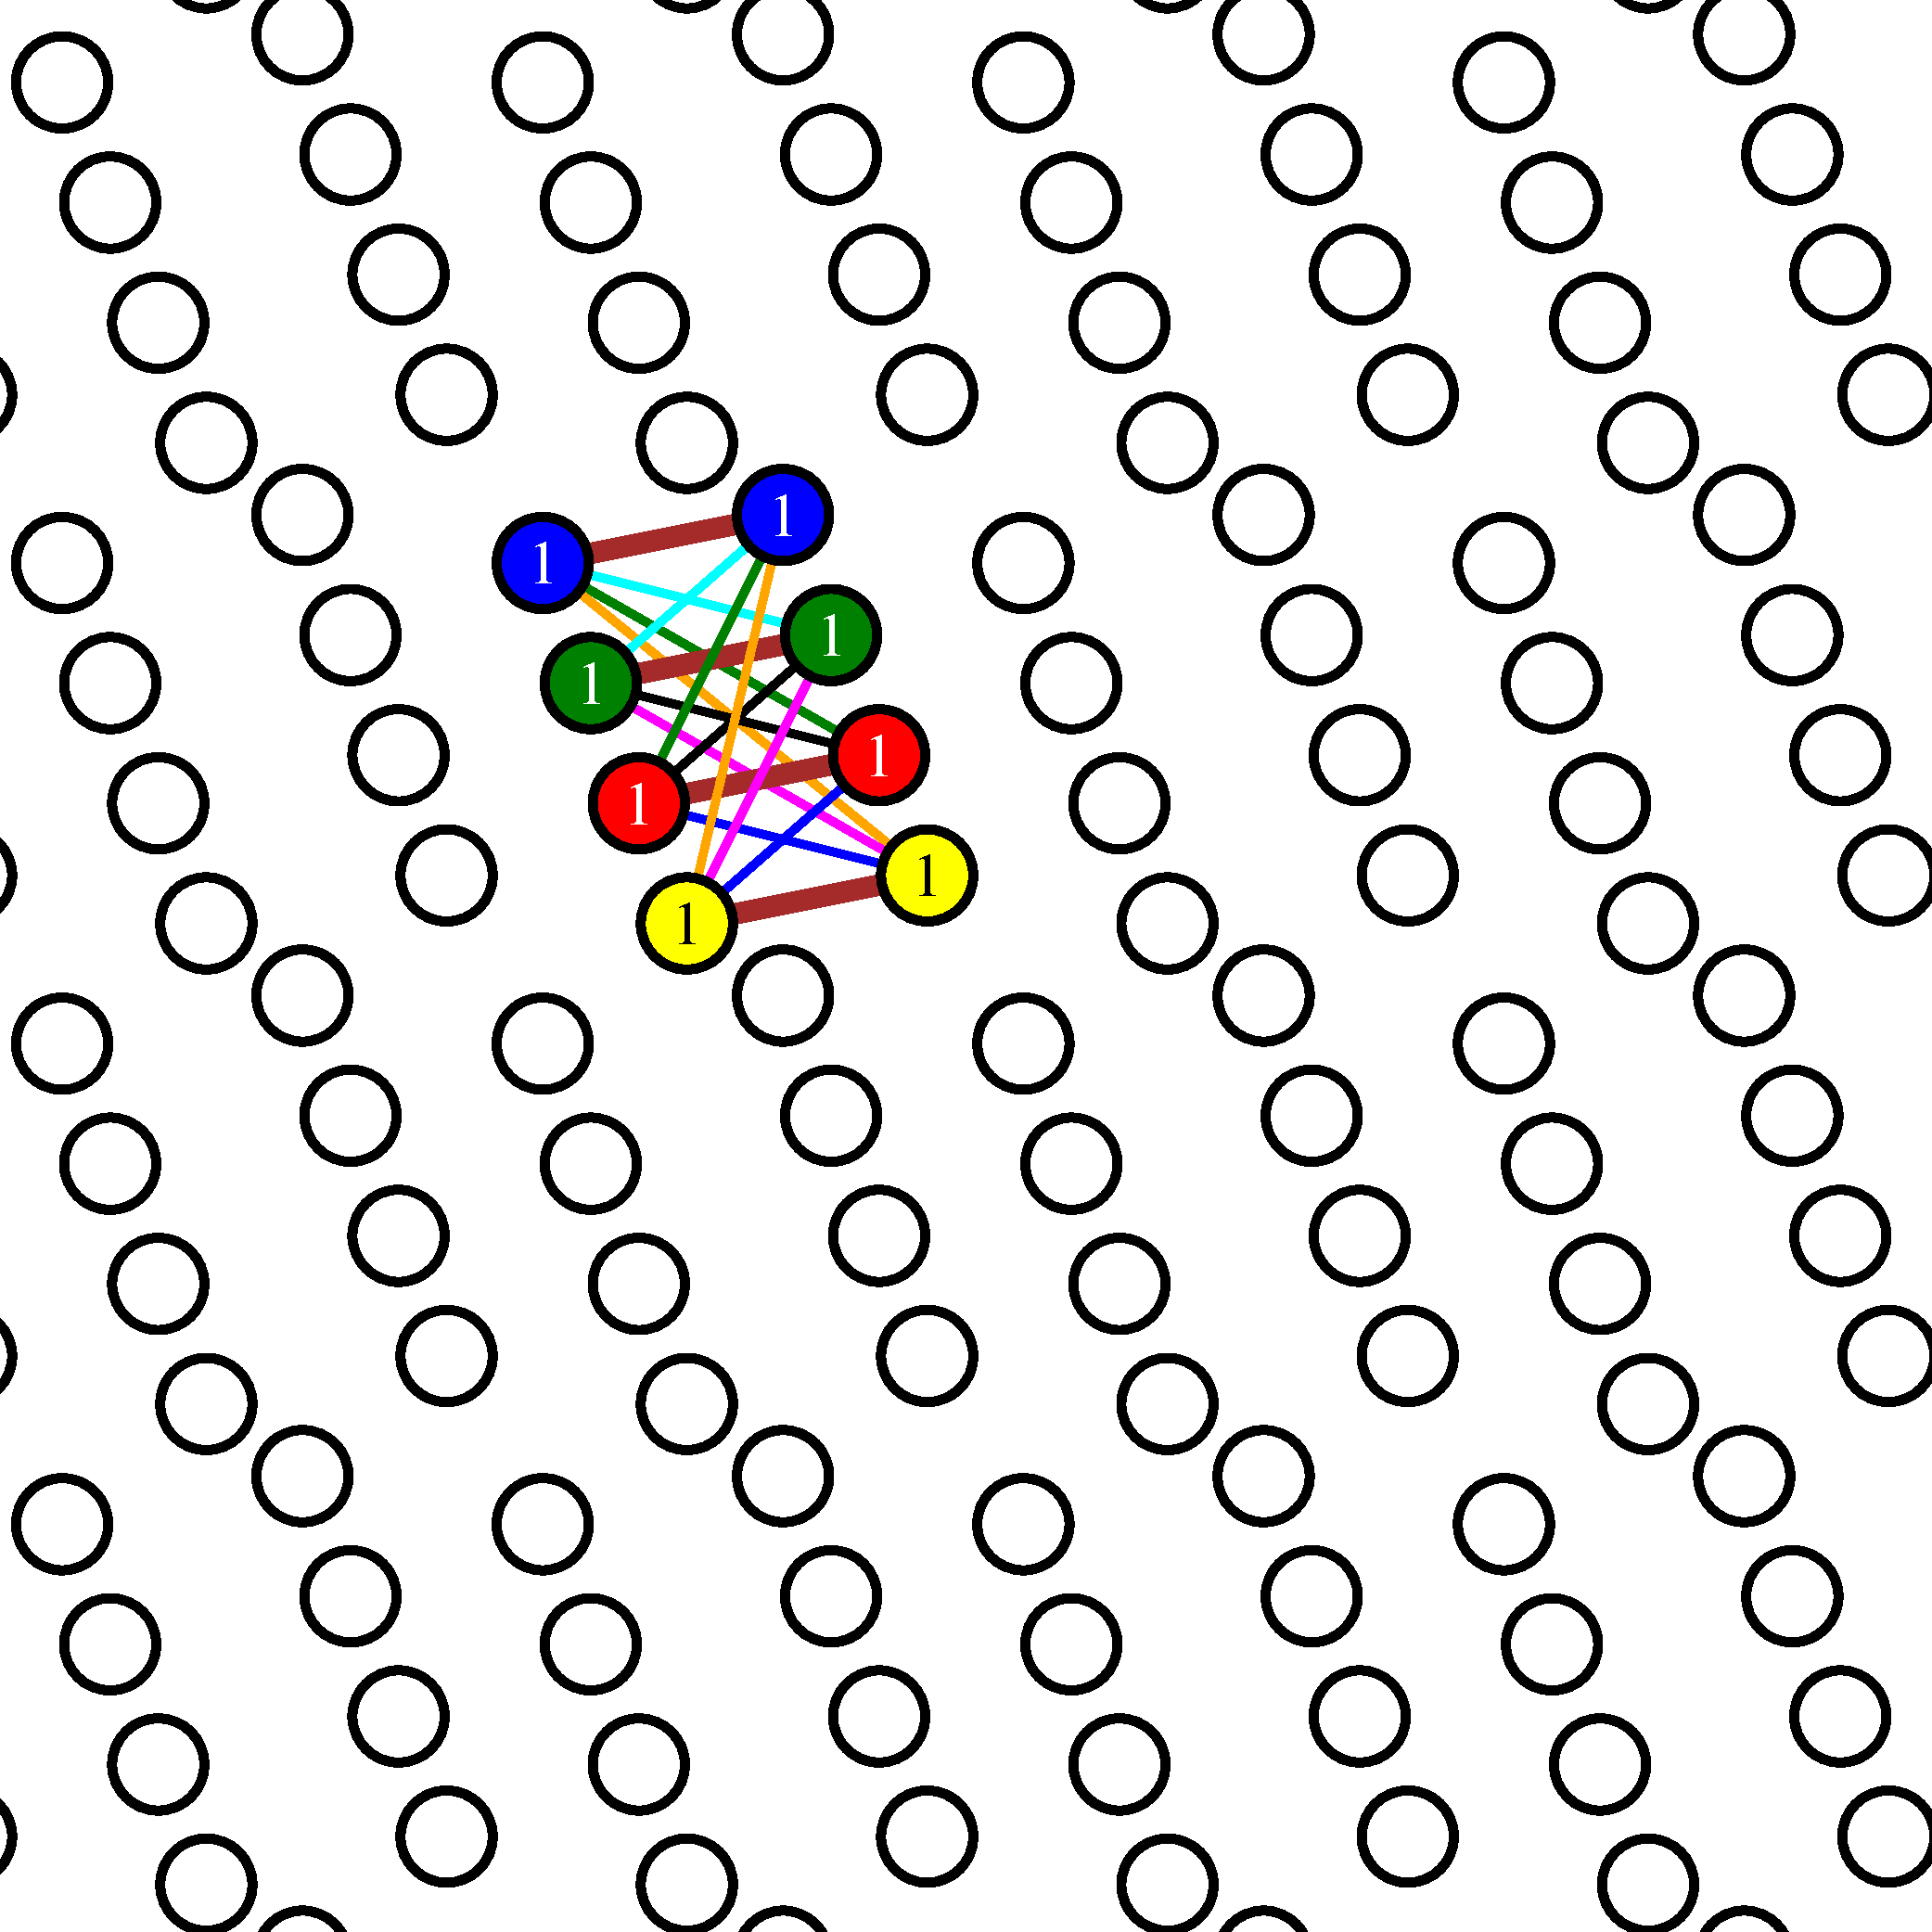
\includegraphics[width=0.23\textwidth]{chapters/Test-driving/4x4_ideal_physical_1}\label{fig:4x4_ideal_physical_1}}
\subfloat[\ Nested graph: 4th level.]{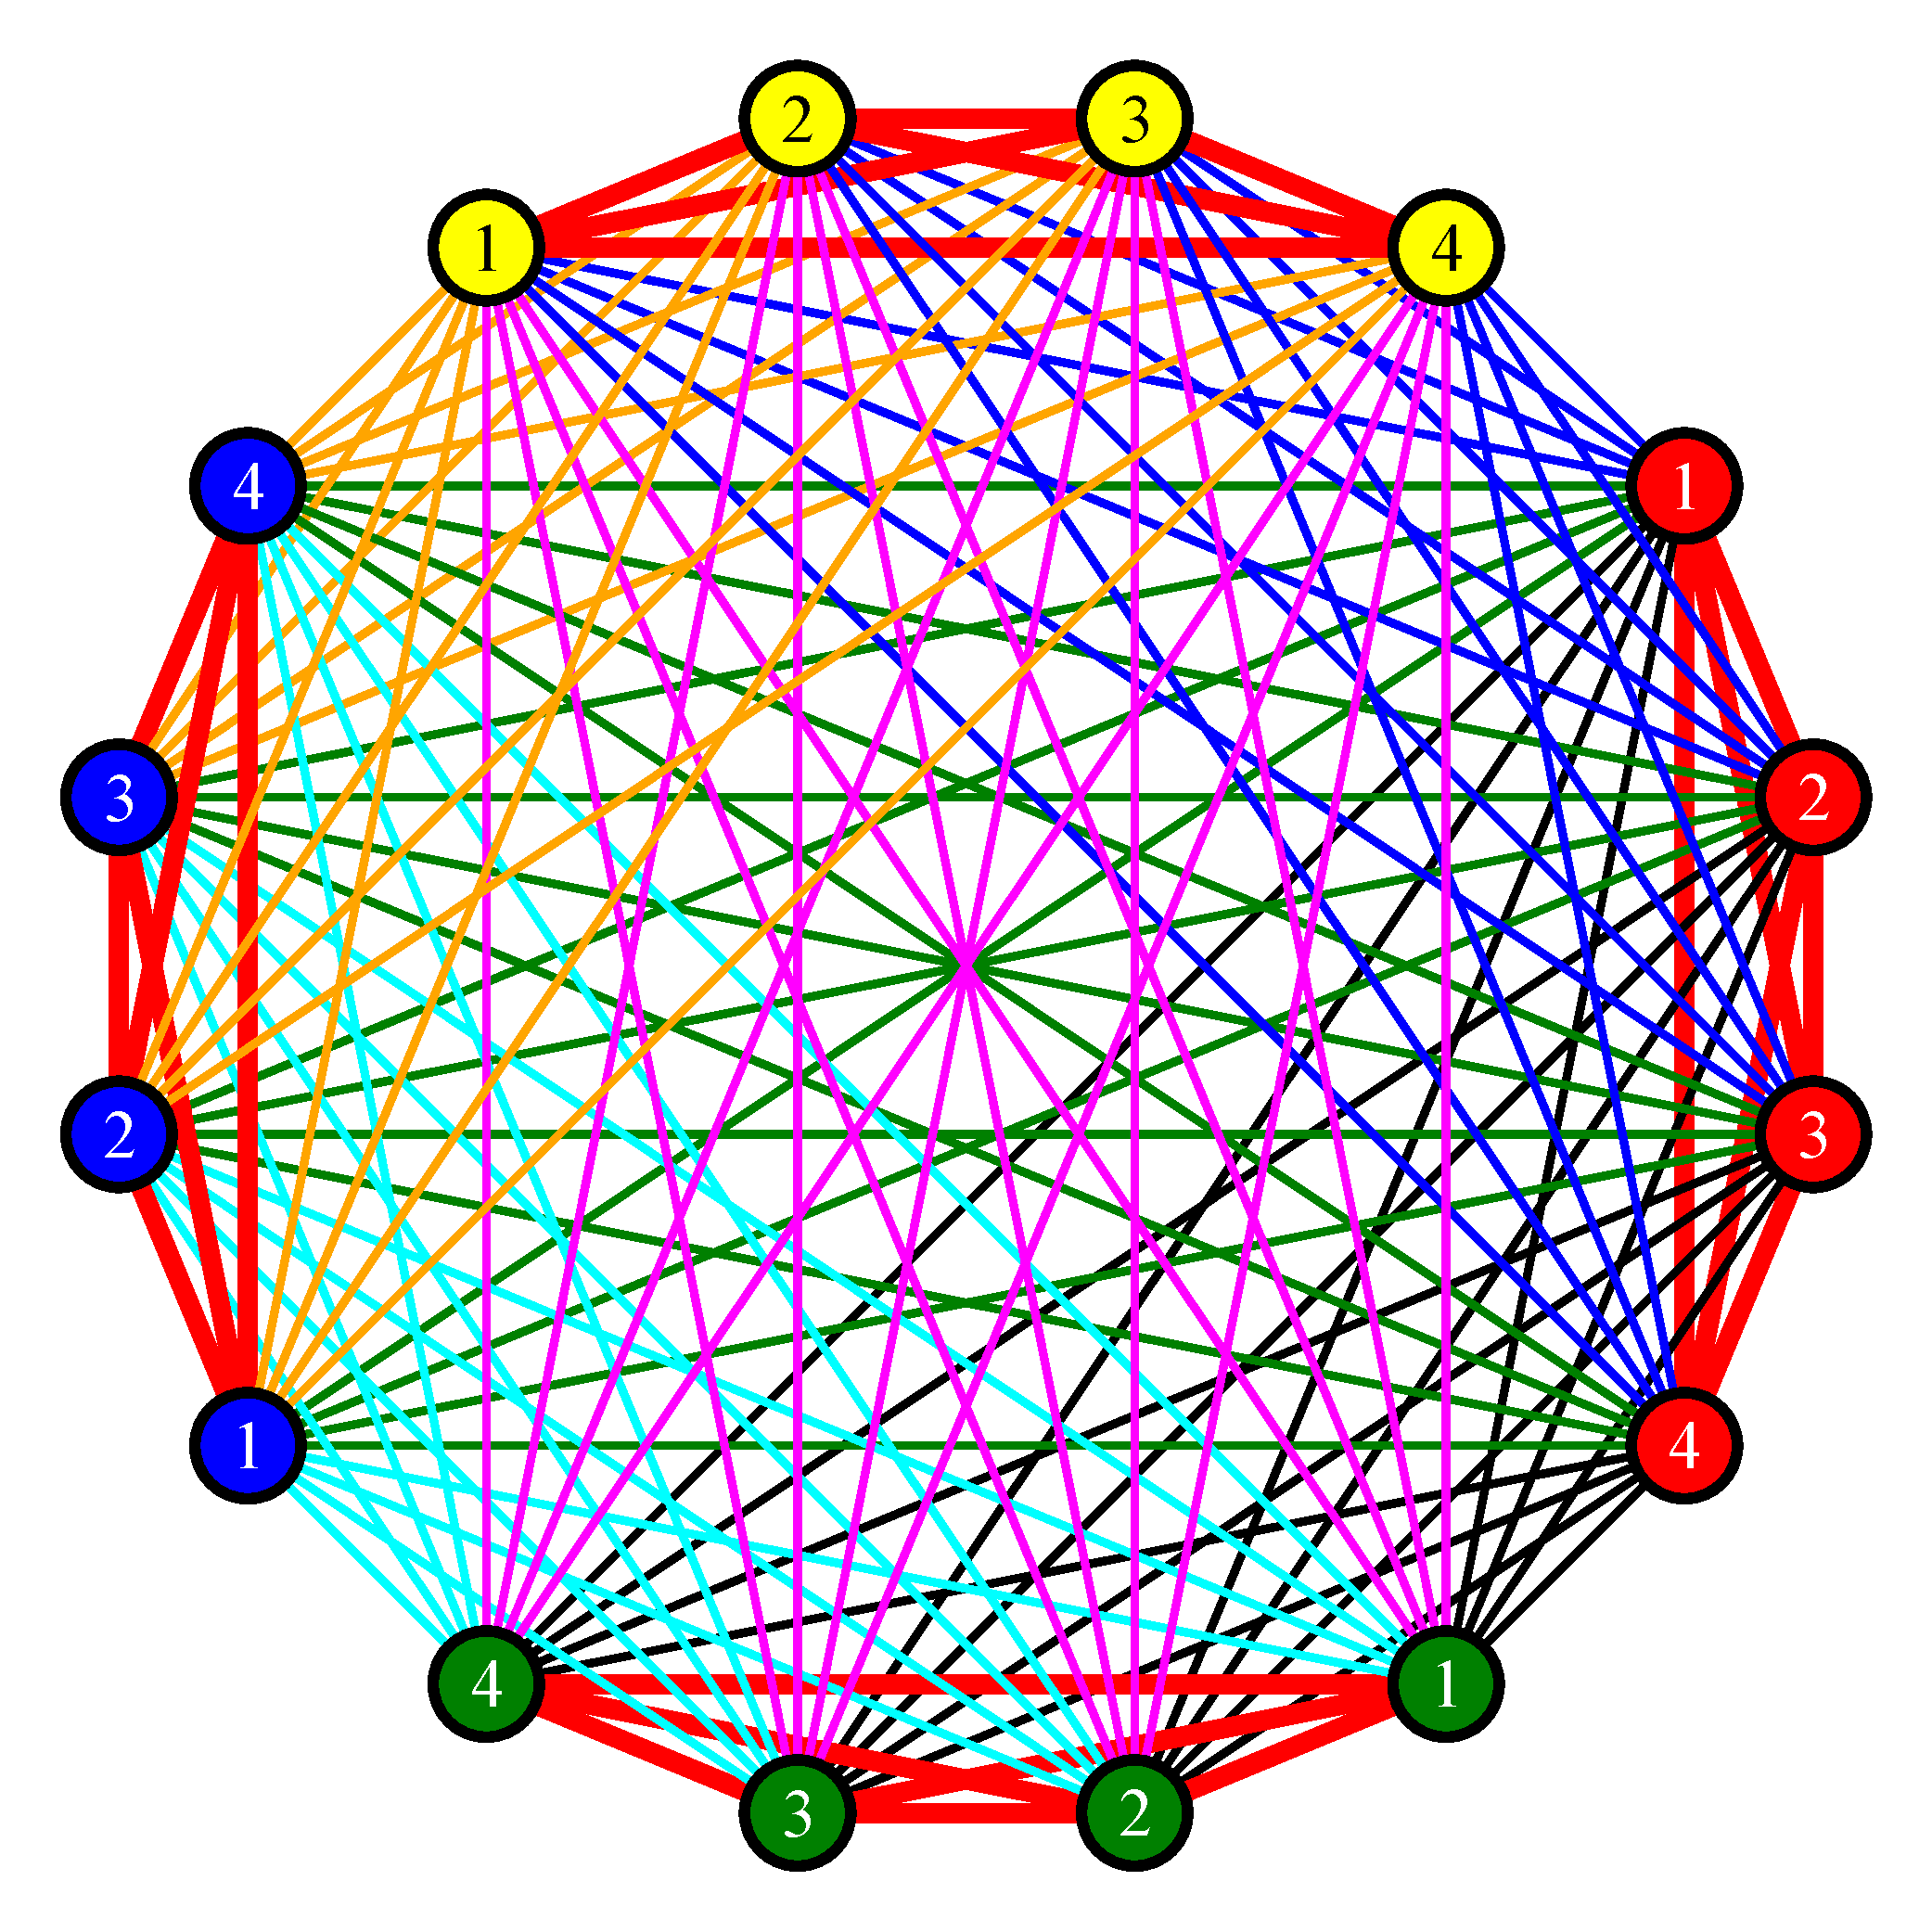
\includegraphics[width=0.23\textwidth]{chapters/Test-driving/4x4_ideal_logical_plot_4}\label{fig:4x4_ideal_logical_plot_4}}
\subfloat[\ 4th level ME.]{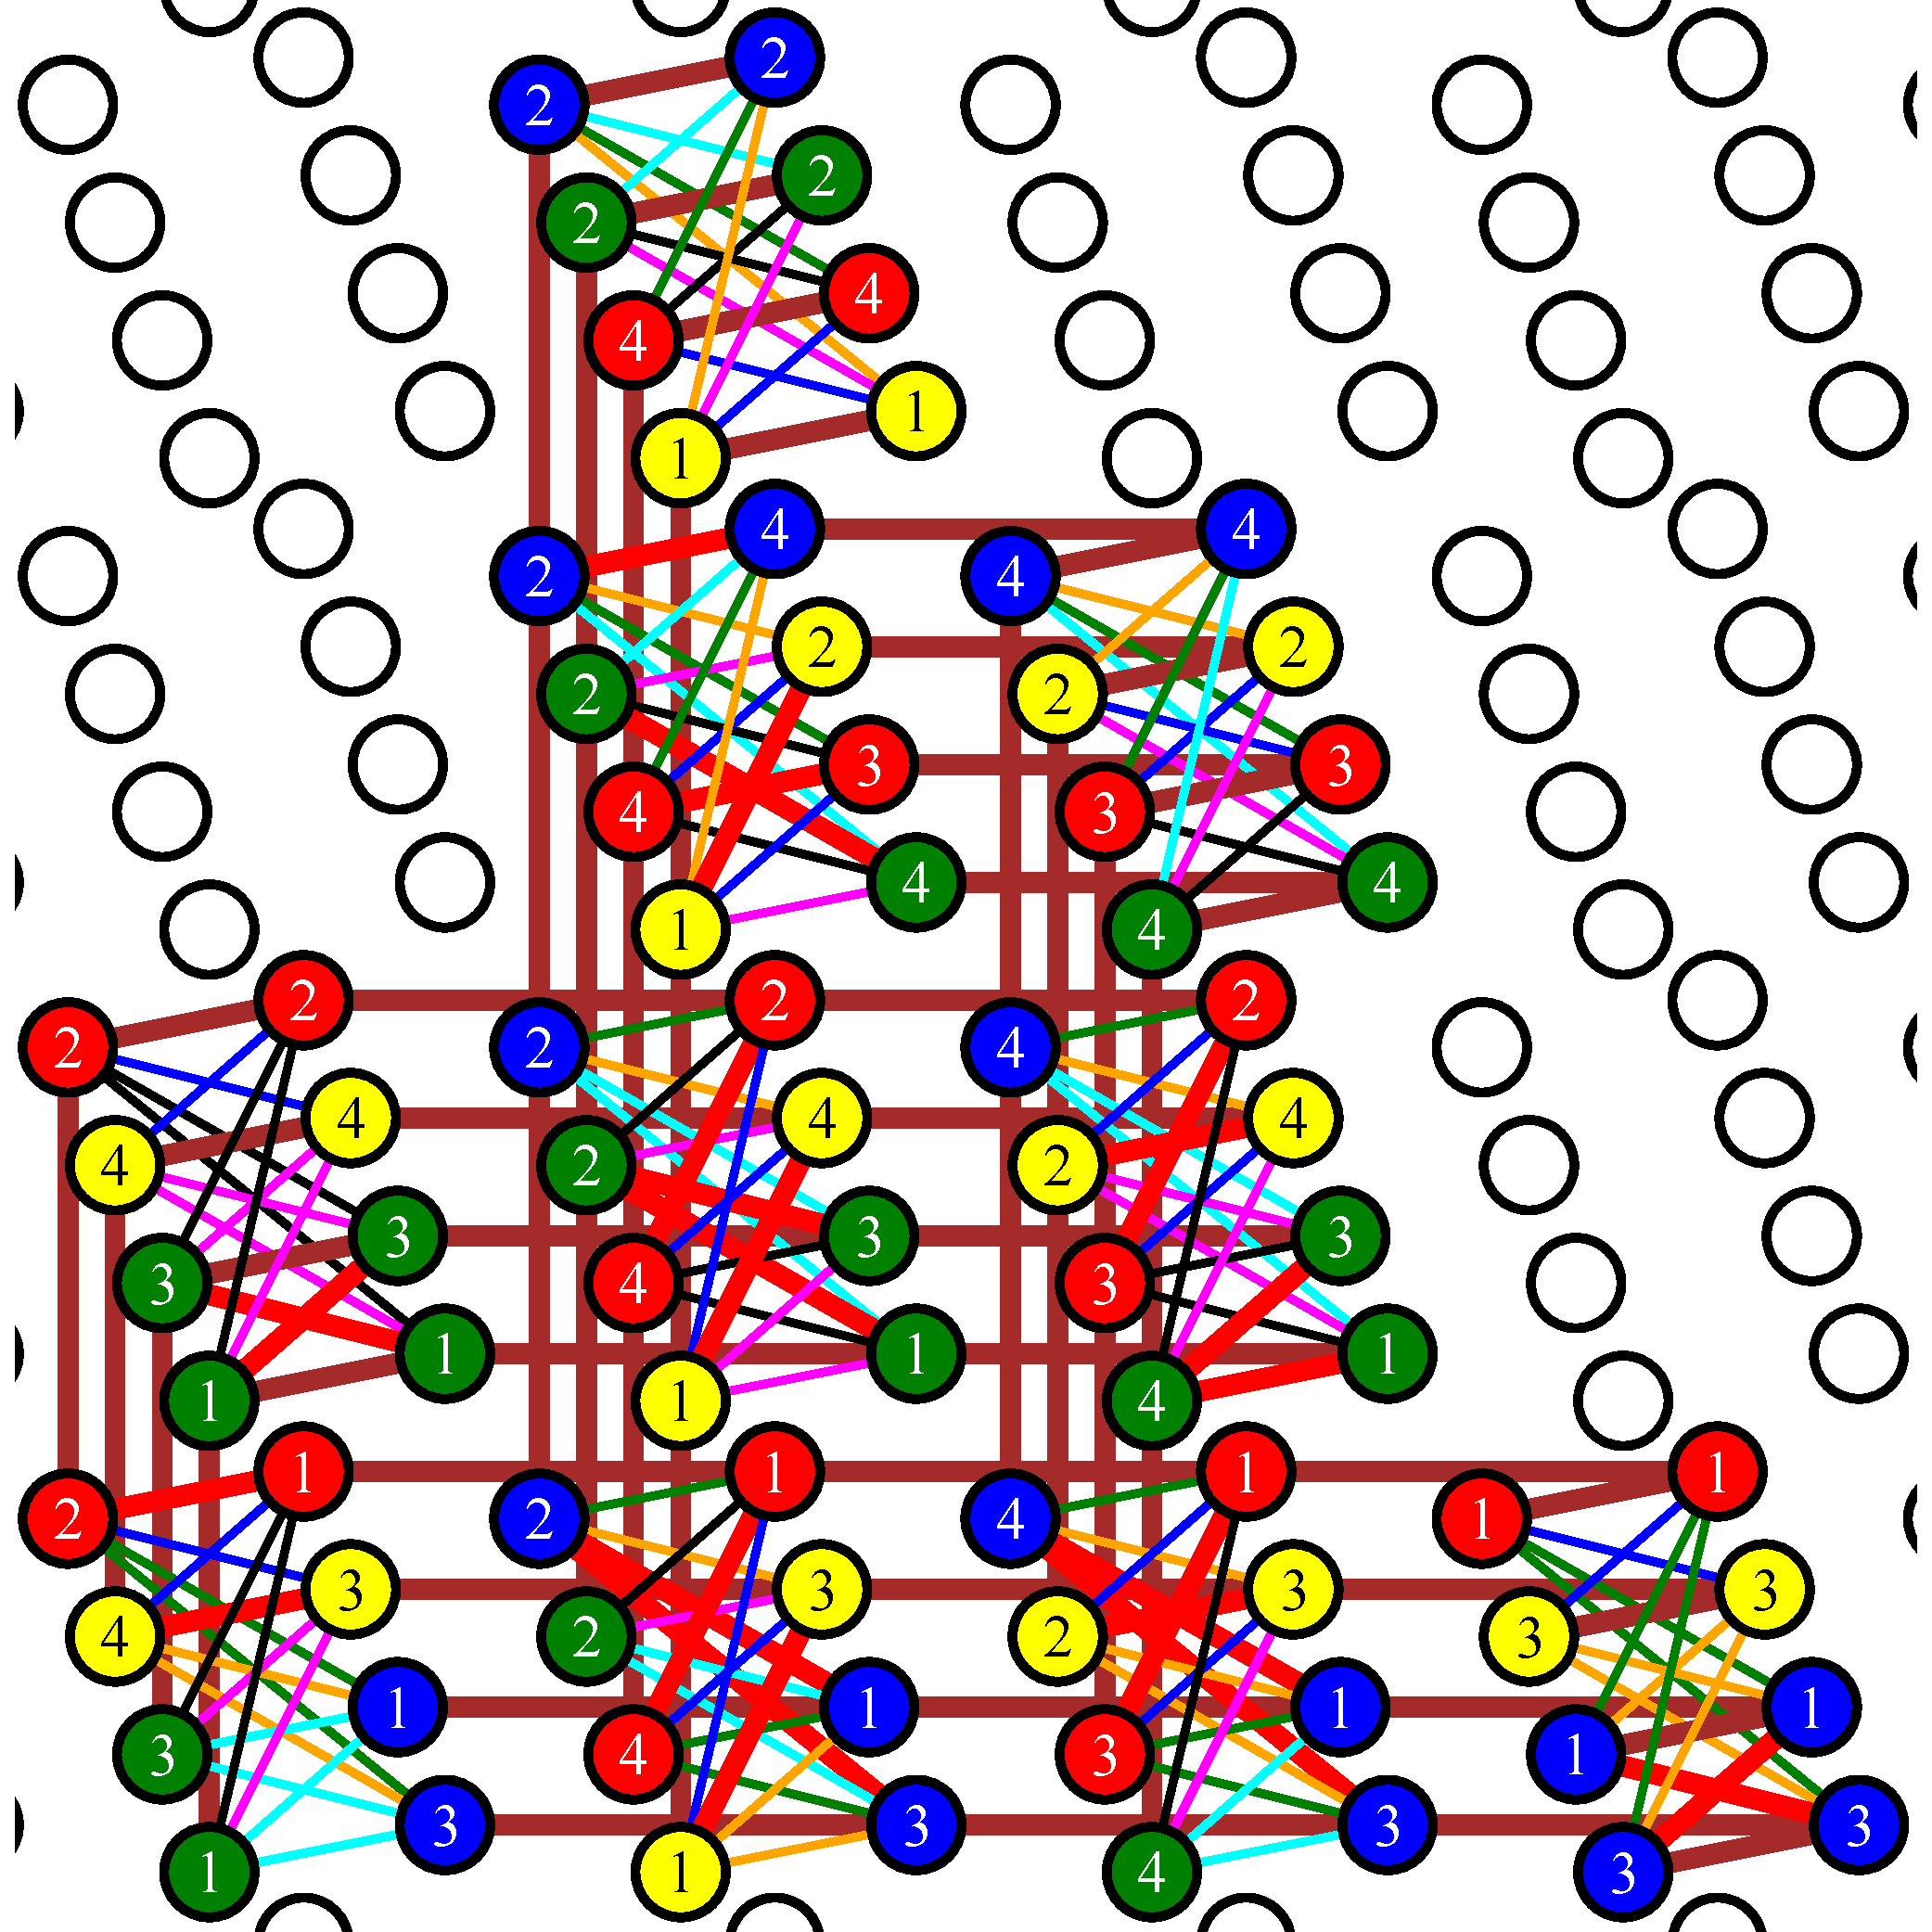
\includegraphics[width=0.23\textwidth]{chapters/Test-driving/4x4_ideal_physical_4}\label{fig:4x4_ideal_physical_4}}
\caption{Illustration of the nested QAC scheme introduced in Ref.~\cite{vinci2015nested}. In the left column, a  $C$-level nested graph is constructed by embedding a $K_N$ into a $K_{C\times N}$, with $N=4$ and $C=1$ (top) and $C=4$ (bottom). Red, thick
couplers are energy penalties defined on the nested graph between the $(i,c)$ nested copies of each logical qubit $i$.
The right column shows the nested graphs after minor embedding (ME) on the DW2X Chimera graph. Brown, thick couplers correspond to the ferromagnetic chains introduced in the process.
}
\label{fig:NQAC}
\end{center}
\end{figure}
%%%%%%

\section{Error Correction}
\label{sec:err-corr}
The discussion of error correction in gate-based quantum computing is usually dominated by questions of fault tolerance and the error thresholds on one and two-qubit gates necessary to satisfy the fault tolerance theorems \cite{Aliferis:05,Raussendorf28092012,Lidar-Brun:book}. The state for quantum annealing and adiabatic quantum computing is quite different, as there is currently no known mechanism for achieving fault tolerance in such devices. Without the benefit of fault tolerance theorems, the best techniques we have available for managing errors in AQC and QA are energy gap protection \cite{jordan2006error}, dynamical decoupling \cite{PhysRevLett.100.160506}, and the Zeno effect \cite{PhysRevLett.108.080501}, three intimately related techniques \cite{Young:13}. Work on error correction in physically realized quantum annealers has focused on energy gap protection, as techniques for dynamical decoupling are unavailable in current generations of annealers due to the associated high bandwidth requirements. Both of these techniques are really more error suppression than correction, as rather then correct errors  they can lower the probability that errors will occur and mitigate their consequences should they happen.

The first demonstration of error suppression via energy energy gap protection in quantum annealers came with the introduction of the technique of quantum annealing correction (QAC) \cite{PAL:13}, which as the name suggests, also includes an active error correction component. In addition, Ref.~\cite{PAL:13} introduced a method for energy boosting by encoding the final Hamiltonian of a quantum annealing algorithm via multiple copies of the logical Hamiltonian operating on separate sets of physical qubits. This is in effect a simple classical repetition code. The copies are bound together by a penalty qubit whose action is to increase the energy of states of the physical system in which the copies are not in alignment with each other. The energy penalty for disagreement between the states effectively suppresses excitation to error states. Figure~\ref{fig:QAC} shows the structure of the encoding and the nature of the encoded problem graph on a DW2 device. The logical Hamiltonian is boosted to have an effective strength three times that achievable in the hardware by directly programming the Hamiltonian. A restriction of this approach is that only the final Hamiltonian is encoded, not the driver Hamiltonian $-\sum \sigma_i^x$, which means that while the final Hamiltonian's gap is significantly larger than in the unencoded case, it is difficult to verify that the minimum ground to first excited state gap of the quantum Hamiltonian is also enhanced. However, a mean field analysis shows that QAC softens the gap closure dependence on system size $N$, in the sense that for models exhibiting a first order quantum phase transition with the gap $\Delta$ scaling as $C^N$, the coefficient $0<C\leq 1$ grows monotonically with the QAC penalty strength $\gamma$, and saturates at $C=1$ for sufficiently large $\gamma$ \cite{MNAL:15,matsuura2017qac}. The same work also showed that after QAC, the free energy barrier between the global minimum and the local minimum the system is initially trapped in is reduced in both width and height for a variety of transverse field Ising spin models, including models with disorder such as the Hopfield model.

The encoding restriction on QAC is not intrinsic to the technique, but rather is the result of the lack of any higher order (more than single-body) $\sigma^x$ terms in the system Hamiltonian, which renders it impossible to form an effective logical $\sigma^x$ term. Decoding a QAC encoded Hamiltonian is as simple as applying a majority vote over the problem qubits. The method was tested in Ref.~\cite{PAL:13} on antiferromagnetic chains of various lengths, demonstrating a significant improvement in success probability of finding the ground state of the chains compared not only to the unencoded case but also the case of a four copy repetition code (since QAC uses four times the hardware resources, one could simply run four copies of the problem at once and pick the lowest energy solution from any copy). As implemented in Ref.~\cite{PAL:13}, the technique is not scalable (in the sense that both the energy boost and the gap against errors is constant), but it provided the first hope for systematically overcoming errors in the experimental quantum annealing. Another innovation was the use of many embeddings of the same logical Hamiltonian into compatible subgraphs, an idea which has found its way into the benchmarking context.

Chains have a trivial (classical) ground state, so a natural next test of QAC was to apply the method to random Ising problem instances \cite{PAL:14}. This provided a  demonstration that QAC could improve performance also on NP-hard problems defined on the QAC logical graph. Moreover, not only was the absolute performance on random Ising problems improved over both the unencoded and the classical repetition cases, but the scaling of the time to solution for those problems improved under QAC, with the caveat that no optimal annealing time was identified. In addition, QAC improved the robustness of the annealer to problem misspecification and increased the effective accuracy of the implemented problem Hamiltonian, as was shown by systematically reducing the energy scale of the final Hamiltonian. Since the hardware graph of the DW2 had missing qubits, encoding Ising problems required that some logical qubits went without a penalty qubit. Additional robustness was thus demonstrated by artificially increasing the number of penalty qubits lost: with up to $60\%$ of the logical qubits going without penalty qubits, QAC continued to work with negligible performance loss.

The next step in testing QAC was to apply it to minor-embedded problems \cite{Vinci:2015jt}, dubbed QAC-ME, thus going beyond natively embeddable problems such as chains and random Ising instances; see Fig.~\ref{fig:square-code}. A key innovation introduced in Ref.~\cite{Vinci:2015jt} is the introduction of non-uniform weights for both the QAC penalty terms as well as the strength of the chain in the minor embedding, making them both proportional to the mean coupling strength in their respective logical Hamiltonians. This was in part informed by previous minor embedding experiments such as Ref.~\cite{Venturelli:2014nx}, in which the optimal strength of the chain was found to be related to the emergence of the spin glass phase of the Hamiltonian. Since there is only a single strength $\sigma^x$ term applied to every qubit while the strength of the $\sigma^z$ terms depends on the choice of $h_i$ and $J_{ij}$, one can easily find that with a uniform penalty strength some qubits will ``freeze'' (i.e., no longer be effectively flipped by the driver Hamiltonian) before others, which can negatively impact solution quality. By locally fitting penalties to the strength of the logical problem Hamiltonian for each qubit, this process can be mitigated. Addressing decoding, Ref.~\cite{Vinci:2015jt} also proposed to use energy minimization, which involves directly minimizing the state of broken logical qubits (logical qubits whose physical qubits are not in alignment) given their neighboring qubits, and demonstrated that this can be done efficiently so long as the per-qubit probability of error is below the percolation threshold of the problem graph. And, going beyond the original QAC code of Ref.~\cite{PAL:13}, a new, scalable QAC ``square code" whose logical graph forms a two-level-grid was proposed in Ref.~\cite{Vinci:2015jt} (see Fig.~\ref{fig:square-code}). The square code has the attractive feature that it can be concatenated. To benchmark QAC-ME, the same kind of frustrated loop problems with planted solutions that were first introduced in Ref.~\cite{Hen:2015rt} were used. The results demonstrated a significant improvement in performance for non-uniform penalties over uniform penalty strengths, and that energy minimization was strongly preferable for decoding QAC-ME compared to standard majority vote decoding. The square code was compared with the original QAC code on chains in Ref.~\cite{Mishra:2015}.

Both the original QAC scheme and QAC-ME induce a graph of lower degree than that of the initial Hamiltonian. To overcome this and deal from the start with arbitrary Ising model Hamiltonians, a ``nested QAC" (NQAC) method was introduced in Ref.~\cite{vinci2015nested}. NQAC starts from a fully connected $K_N$ graph for the underlying problem and then maps this $N$ qubit problem into $C$ coupled copies of itself in a larger $K_{C\times N}$ graph. When run on a hardware graph of lower degree, this larger $K_{C\times N}$ graph is then minor-embedded, with the coupled copies doing the work of suppressing errors and helping to limit the formation of domain walls in the minor embedding chains. In this way, the number of physical qubits required to implement level-$C$ NQAC is approximately $C^2 N^2/4$. An illustration of the embedding of the $K_N$ Hamiltonian into the larger $K_{C\times N}$ Hamiltonian as well as a sample of the minor embedded graph are given in Fig.~\ref{fig:NQAC}.

The key finding of Ref.~\cite{vinci2015nested} is that NQAC effectively rescales the temperature of the system down by a factor of $\mu_C$ for $C$ nesting levels, with the theoretical expectation for a fully thermalized state being that $\mu_C\propto C^2$, based on a mean-field analysis. In practice, the scaling is not quite that fast, instead $\mu_C\approx C^{1.4}$ once the energy penalty tying the $C$ copies of the problem Hamiltonian together and the chain strength are optimized. This result is important since it means that one can trade qubits for an effective temperature reduction, that is controllable via the nesting level $C$. This suggests, at least in principle, that the effective temperature can be kept below the gap. For the DW2 device, for $C\geq 3$ NQAC was no longer able to improve the success probability more than classical repetition of the $C=1$ case, though this is probably because the base problem (a random antiferromagnetic Ising $K_8$ with $J_{ij}\in\{0.1,0.2,\dots,1\}$) was too easy. Tests on more advanced processors such as the DW2KQ and beyond will reveal whether techniques like NQAC hold at least part of the key to scalable quantum error suppression and correction on quantum annealing platforms, even if it and similar pure error suppression techniques will never be able to achieve true fault tolerance.

The story of error suppression and correction in experimental quantum annealing algorithms is one of a sequence of developments, building off both the results and lessons of native benchmarking work and the initial insight of energy gap protection as a fruitful and feasible path on current systems for error suppression, and generalizing to more and more useful encoded graphs, until finally reaching NQAC with its fully general encoded Ising Hamiltonian and potential for arbitrarily large and strong error suppression. Future paths for investigation of experimental quantum annealing correction center on expanded benchmarking of NQAC for larger systems and for application-domain problems, as well as continued theoretical development of error suppression and correction techniques. For example, using subsystem codes it is possible to construct error suppression schemes appropriate for adiabatic quantum computing that use only two-body interactions, so that by adding $\sigma^x_i \sigma^x_j$ terms to the driver Hamiltonian one could significantly improve over the current state of the art of QAC  \cite{Marvian-Lidar:16,Jiang:2015kx}.


\section{Conclusion}
As the field of quantum computing, and quantum annealing in particular, expands rapidly and the number of available platforms rises, methods to validate the fidelity of the platform to its stated physical model, verifying entanglement and tunneling, strong benchmarking methods, and error correction/suppression techniques will be vital in discerning which platforms truly can offer advantages over classical computation. Several years have been spent developing methods to meet each of these challenges, particularly targeting existing quantum annealers, but many of these methods can be readily adapted to other systems that implement programmable Ising model Hamiltonians \cite{Inagaki:2016aa}. Insights from each of these areas are informing development in the others. For example, insight into and experience with small gadgets from quantum validation informed recent work demonstrating a limited quantum speedup on D-Wave quantum annealers using a small gadget to generate an optimal annealing time on existing machines, while insights from benchmarking regularly inform developments in error suppression and correction. Work on benchmarking has provided guidelines and methods of analysis which can be used by anyone seeking to characterize the performance of a putative quantum computing device, while error suppression work has laid the foundation for more extensive experiments and solving more difficult problems on future, larger quantum annealing devices. Thus, one answer to the question of what one may want to use a $1000$-qubit quantum computer for, is in our view the type of bootstrapping we have reviewed in this article, where a productive interplay among quantum validation testing, benchmarking, and error correction has led to a sequence of advances that will inform even larger quantum computation experiments, until one day a test drive with a brand new quantum computer will take us to the ultimate destination of undisputed quantum supremacy and unqualifed quantum speedup.


\vspace{.8cm}

\textbf{Acknowledgements}

We are grateful to the many colleagues with whom we have collaborated over the past several years of test-driving quantum annealers, and in particular to Tameem Albash for helpful discussions and comments on this article, and to Siddharth Muthu Krishnan for prompting us to write this review. This work was supported under ARO grant number W911NF-12-1-0523, ARO MURI grant No. W911NF-15-1-0582, and NSF grant number INSPIRE-1551064.

%merlin.mbs apsrev4-1.bst 2010-07-25 4.21a (PWD, AO, DPC) hacked
%Control: key (0)
%Control: author (8) initials jnrlst
%Control: editor formatted (1) identically to author
%Control: production of article title (-1) disabled
%Control: page (0) single
%Control: year (1) truncated
%Control: production of eprint (0) enabled
% \begin{thebibliography}{101}%
% \makeatletter
% \providecommand \@ifxundefined [1]{%
%  \@ifx{#1\undefined}
% }%
% \providecommand \@ifnum [1]{%
%  \ifnum #1\expandafter \@firstoftwo
%  \else \expandafter \@secondoftwo
%  \fi
% }%
% \providecommand \@ifx [1]{%
%  \ifx #1\expandafter \@firstoftwo
%  \else \expandafter \@secondoftwo
%  \fi
% }%
% \providecommand \natexlab [1]{#1}%
% \providecommand \enquote  [1]{``#1''}%
% \providecommand \bibnamefont  [1]{#1}%
% \providecommand \bibfnamefont [1]{#1}%
% \providecommand \citenamefont [1]{#1}%
% \providecommand \href@noop [0]{\@secondoftwo}%
% \providecommand \href [0]{\begingroup \@sanitize@url \@href}%
% \providecommand \@href[1]{\@@startlink{#1}\@@href}%
% \providecommand \@@href[1]{\endgroup#1\@@endlink}%
% \providecommand \@sanitize@url [0]{\catcode `\\12\catcode `\$12\catcode
%   `\&12\catcode `\#12\catcode `\^12\catcode `\_12\catcode `\%12\relax}%
% \providecommand \@@startlink[1]{}%
% \providecommand \@@endlink[0]{}%
% \providecommand \url  [0]{\begingroup\@sanitize@url \@url }%
% \providecommand \@url [1]{\endgroup\@href {#1}{\urlprefix }}%
% \providecommand \urlprefix  [0]{URL }%
% \providecommand \Eprint [0]{\href }%
% \providecommand \doibase [0]{http://dx.doi.org/}%
% \providecommand \selectlanguage [0]{\@gobble}%
% \providecommand \bibinfo  [0]{\@secondoftwo}%
% \providecommand \bibfield  [0]{\@secondoftwo}%
% \providecommand \translation [1]{[#1]}%
% \providecommand \BibitemOpen [0]{}%
% \providecommand \bibitemStop [0]{}%
% \providecommand \bibitemNoStop [0]{.\EOS\space}%
% \providecommand \EOS [0]{\spacefactor3000\relax}%
% \providecommand \BibitemShut  [1]{\csname bibitem#1\endcsname}%
% \let\auto@bib@innerbib\@empty
% %</preamble>
% \bibitem [{\citenamefont {Reichardt}\ \emph {et~al.}(2013)\citenamefont
%   {Reichardt}, \citenamefont {Unger},\ and\ \citenamefont
%   {Vazirani}}]{Reichardt:2013db}%
%   \BibitemOpen
%   \bibfield  {author} {\bibinfo {author} {\bibfnamefont {B.~W.}\ \bibnamefont
%   {Reichardt}}, \bibinfo {author} {\bibfnamefont {F.}~\bibnamefont {Unger}}, \
%   and\ \bibinfo {author} {\bibfnamefont {U.}~\bibnamefont {Vazirani}},\ }\href
%   {\doibase 10.1038/nature12035} {\bibfield  {journal} {\bibinfo  {journal}
%   {Nature}\ }\textbf {\bibinfo {volume} {496}},\ \bibinfo {pages} {456}
%   (\bibinfo {year} {2013})}\BibitemShut {NoStop}%
% \bibitem [{\citenamefont {Chuang}\ and\ \citenamefont
%   {Nielsen}(1997)}]{Chuang:97c}%
%   \BibitemOpen
%   \bibfield  {author} {\bibinfo {author} {\bibfnamefont {I.~L.}\ \bibnamefont
%   {Chuang}}\ and\ \bibinfo {author} {\bibfnamefont {M.~A.}\ \bibnamefont
%   {Nielsen}},\ }\bibfield  {booktitle} {\emph {\bibinfo {booktitle} {Journal of
%   Modern Optics}},\ }\href
%   {http://www.tandfonline.com/doi/abs/10.1080/09500349708231894} {\bibfield
%   {journal} {\bibinfo  {journal} {Journal of Modern Optics}\ }\textbf {\bibinfo
%   {volume} {44}},\ \bibinfo {pages} {2455} (\bibinfo {year}
%   {1997})}\BibitemShut {NoStop}%
% \bibitem [{\citenamefont {Mohseni}\ \emph {et~al.}(2008)\citenamefont
%   {Mohseni}, \citenamefont {Rezakhani},\ and\ \citenamefont
%   {Lidar}}]{Mohseni:2008ly}%
%   \BibitemOpen
%   \bibfield  {author} {\bibinfo {author} {\bibfnamefont {M.}~\bibnamefont
%   {Mohseni}}, \bibinfo {author} {\bibfnamefont {A.~T.}\ \bibnamefont
%   {Rezakhani}}, \ and\ \bibinfo {author} {\bibfnamefont {D.~A.}\ \bibnamefont
%   {Lidar}},\ }\href {http://link.aps.org/doi/10.1103/PhysRevA.77.032322}
%   {\bibfield  {journal} {\bibinfo  {journal} {Phys. Rev. A}\ }\textbf {\bibinfo
%   {volume} {77}},\ \bibinfo {pages} {032322} (\bibinfo {year}
%   {2008})}\BibitemShut {NoStop}%
% \bibitem [{\citenamefont {Blume-Kohout}\ \emph {et~al.}(2013)\citenamefont
%   {Blume-Kohout}, \citenamefont {Gamble}, \citenamefont {Nielsen},
%   \citenamefont {Mizrahi}, \citenamefont {Sterk},\ and\ \citenamefont
%   {Maunz}}]{blume2013robust}%
%   \BibitemOpen
%   \bibfield  {author} {\bibinfo {author} {\bibfnamefont {R.}~\bibnamefont
%   {Blume-Kohout}}, \bibinfo {author} {\bibfnamefont {J.~K.}\ \bibnamefont
%   {Gamble}}, \bibinfo {author} {\bibfnamefont {E.}~\bibnamefont {Nielsen}},
%   \bibinfo {author} {\bibfnamefont {J.}~\bibnamefont {Mizrahi}}, \bibinfo
%   {author} {\bibfnamefont {J.~D.}\ \bibnamefont {Sterk}}, \ and\ \bibinfo
%   {author} {\bibfnamefont {P.}~\bibnamefont {Maunz}},\ }\href
%   {http://arXiv.org/abs/1310.4492} {\bibfield  {journal} {\bibinfo  {journal}
%   {arXiv:1310.4492}\ } (\bibinfo {year} {2013})}\BibitemShut {NoStop}%
% \bibitem [{\citenamefont {Greenbaum}(2015)}]{Greenbaum:2015aa}%
%   \BibitemOpen
%   \bibfield  {author} {\bibinfo {author} {\bibfnamefont {D.}~\bibnamefont
%   {Greenbaum}},\ }\href {http://arXiv.org/abs/1509.02921} {\bibfield  {journal}
%   {\bibinfo  {journal} {arXiv:1509.02921}\ } (\bibinfo {year}
%   {2015})}\BibitemShut {NoStop}%
% \bibitem [{\citenamefont {Childs}\ \emph {et~al.}(2001)\citenamefont {Childs},
%   \citenamefont {Chuang},\ and\ \citenamefont {Leung}}]{Childs:00}%
%   \BibitemOpen
%   \bibfield  {author} {\bibinfo {author} {\bibfnamefont {A.~M.}\ \bibnamefont
%   {Childs}}, \bibinfo {author} {\bibfnamefont {I.~L.}\ \bibnamefont {Chuang}},
%   \ and\ \bibinfo {author} {\bibfnamefont {D.~W.}\ \bibnamefont {Leung}},\
%   }\href {https://link.aps.org/doi/10.1103/PhysRevA.64.012314} {\bibfield
%   {journal} {\bibinfo  {journal} {Physical Review A}\ }\textbf {\bibinfo
%   {volume} {64}},\ \bibinfo {pages} {012314} (\bibinfo {year}
%   {2001})}\BibitemShut {NoStop}%
% \bibitem [{\citenamefont {Blume-Kohout}\ \emph {et~al.}(2017)\citenamefont
%   {Blume-Kohout}, \citenamefont {Gamble}, \citenamefont {Nielsen},
%   \citenamefont {Rudinger}, \citenamefont {Mizrahi}, \citenamefont {Fortier},\
%   and\ \citenamefont {Maunz}}]{Blume-Kohout:2017aa}%
%   \BibitemOpen
%   \bibfield  {author} {\bibinfo {author} {\bibfnamefont {R.}~\bibnamefont
%   {Blume-Kohout}}, \bibinfo {author} {\bibfnamefont {J.~K.}\ \bibnamefont
%   {Gamble}}, \bibinfo {author} {\bibfnamefont {E.}~\bibnamefont {Nielsen}},
%   \bibinfo {author} {\bibfnamefont {K.}~\bibnamefont {Rudinger}}, \bibinfo
%   {author} {\bibfnamefont {J.}~\bibnamefont {Mizrahi}}, \bibinfo {author}
%   {\bibfnamefont {K.}~\bibnamefont {Fortier}}, \ and\ \bibinfo {author}
%   {\bibfnamefont {P.}~\bibnamefont {Maunz}},\ }\href
%   {http://dx.doi.org/10.1038/ncomms14485} {\bibfield  {journal} {\bibinfo
%   {journal} {Nature Communications}\ }\textbf {\bibinfo {volume} {8}},\
%   \bibinfo {pages} {14485} (\bibinfo {year} {2017})}\BibitemShut {NoStop}%
% \bibitem [{\citenamefont {Kadowaki}\ and\ \citenamefont
%   {Nishimori}(1998)}]{kadowaki_quantum_1998}%
%   \BibitemOpen
%   \bibfield  {author} {\bibinfo {author} {\bibfnamefont {T.}~\bibnamefont
%   {Kadowaki}}\ and\ \bibinfo {author} {\bibfnamefont {H.}~\bibnamefont
%   {Nishimori}},\ }\href
%   {http://journals.aps.org/pre/abstract/10.1103/PhysRevE.58.5355} {\bibfield
%   {journal} {\bibinfo  {journal} {Phys. Rev. E}\ }\textbf {\bibinfo {volume}
%   {58}},\ \bibinfo {pages} {5355} (\bibinfo {year} {1998})}\BibitemShut
%   {NoStop}%
% \bibitem [{\citenamefont {Das}\ and\ \citenamefont
%   {Chakrabarti}(2008)}]{RevModPhys.80.1061}%
%   \BibitemOpen
%   \bibfield  {author} {\bibinfo {author} {\bibfnamefont {A.}~\bibnamefont
%   {Das}}\ and\ \bibinfo {author} {\bibfnamefont {B.~K.}\ \bibnamefont
%   {Chakrabarti}},\ }\href {\doibase 10.1103/RevModPhys.80.1061} {\bibfield
%   {journal} {\bibinfo  {journal} {Rev. Mod. Phys.}\ }\textbf {\bibinfo {volume}
%   {80}},\ \bibinfo {pages} {1061} (\bibinfo {year} {2008})}\BibitemShut
%   {NoStop}%
% \bibitem [{\citenamefont {Farhi}\ \emph {et~al.}(2001)\citenamefont {Farhi},
%   \citenamefont {Goldstone}, \citenamefont {Gutmann}, \citenamefont {Lapan},
%   \citenamefont {Lundgren},\ and\ \citenamefont {Preda}}]{farhi2001quantum}%
%   \BibitemOpen
%   \bibfield  {author} {\bibinfo {author} {\bibfnamefont {E.}~\bibnamefont
%   {Farhi}}, \bibinfo {author} {\bibfnamefont {J.}~\bibnamefont {Goldstone}},
%   \bibinfo {author} {\bibfnamefont {S.}~\bibnamefont {Gutmann}}, \bibinfo
%   {author} {\bibfnamefont {J.}~\bibnamefont {Lapan}}, \bibinfo {author}
%   {\bibfnamefont {A.}~\bibnamefont {Lundgren}}, \ and\ \bibinfo {author}
%   {\bibfnamefont {D.}~\bibnamefont {Preda}},\ }\href
%   {http://science.sciencemag.org/content/292/5516/472} {\bibfield  {journal}
%   {\bibinfo  {journal} {Science}\ }\textbf {\bibinfo {volume} {292}},\ \bibinfo
%   {pages} {472} (\bibinfo {year} {2001})}\BibitemShut {NoStop}%
% \bibitem [{\citenamefont {{Kaminsky}}\ and\ \citenamefont
%   {{Lloyd}}(2004)}]{2002quant.ph.11152K}%
%   \BibitemOpen
%   \bibfield  {author} {\bibinfo {author} {\bibfnamefont {W.~M.}\ \bibnamefont
%   {{Kaminsky}}}\ and\ \bibinfo {author} {\bibfnamefont {S.}~\bibnamefont
%   {{Lloyd}}},\ }in\ \href {http://arxiv.org/abs/quant-ph/0211152} {\emph
%   {\bibinfo {booktitle} {Quantum Computing and Quantum Bits in Mesoscopic
%   Systems}}},\ \bibinfo {editor} {edited by\ \bibinfo {editor} {\bibfnamefont
%   {A.}~\bibnamefont {Leggett}}, \bibinfo {editor} {\bibfnamefont
%   {B.}~\bibnamefont {Ruggiero}}, \ and\ \bibinfo {editor} {\bibfnamefont
%   {P.}~\bibnamefont {Silvestrini}}}\ (\bibinfo  {publisher} {Kluwer
%   Academic/Plenum Publ.},\ \bibinfo {year} {2004})\ \Eprint
%   {http://arxiv.org/abs/arXiv:quant-ph/0211152} {arXiv:quant-ph/0211152}
%   \BibitemShut {NoStop}%
% \bibitem [{\citenamefont {Kaminsky}\ \emph {et~al.}(2004)\citenamefont
%   {Kaminsky}, \citenamefont {Lloyd},\ and\ \citenamefont
%   {Orlando}}]{Kaminsky:2004fk}%
%   \BibitemOpen
%   \bibfield  {author} {\bibinfo {author} {\bibfnamefont {W.~M.}\ \bibnamefont
%   {Kaminsky}}, \bibinfo {author} {\bibfnamefont {S.}~\bibnamefont {Lloyd}}, \
%   and\ \bibinfo {author} {\bibfnamefont {T.~P.}\ \bibnamefont {Orlando}},\
%   }\href {http://arXiv.org/abs/quant-ph/0403090} {\bibfield  {journal}
%   {\bibinfo  {journal} {arXiv:quant-ph/0403090}\ } (\bibinfo {year}
%   {2004})}\BibitemShut {NoStop}%
% \bibitem [{\citenamefont {Albash}\ and\ \citenamefont
%   {Lidar}(2016)}]{Albash-Lidar:RMP}%
%   \BibitemOpen
%   \bibfield  {author} {\bibinfo {author} {\bibfnamefont {T.}~\bibnamefont
%   {Albash}}\ and\ \bibinfo {author} {\bibfnamefont {D.~A.}\ \bibnamefont
%   {Lidar}},\ }\href {http://arXiv.org/abs/1611.04471} {\bibfield  {journal}
%   {\bibinfo  {journal} {arXiv:1611.04471}\ } (\bibinfo {year}
%   {2016})}\BibitemShut {NoStop}%
% \bibitem [{\citenamefont {Berkley}\ \emph {et~al.}(2013)\citenamefont
%   {Berkley}, \citenamefont {Przybysz}, \citenamefont {Lanting}, \citenamefont
%   {Harris}, \citenamefont {Dickson}, \citenamefont {Altomare}, \citenamefont
%   {Amin}, \citenamefont {Bunyk}, \citenamefont {Enderud}, \citenamefont
%   {Hoskinson}, \citenamefont {Johnson}, \citenamefont {Ladizinsky},
%   \citenamefont {Neufeld}, \citenamefont {Rich}, \citenamefont {Smirnov},
%   \citenamefont {Tolkacheva}, \citenamefont {Uchaikin},\ and\ \citenamefont
%   {Wilson}}]{Berkley:2013bf}%
%   \BibitemOpen
%   \bibfield  {author} {\bibinfo {author} {\bibfnamefont {A.~J.}\ \bibnamefont
%   {Berkley}}, \bibinfo {author} {\bibfnamefont {A.~J.}\ \bibnamefont
%   {Przybysz}}, \bibinfo {author} {\bibfnamefont {T.}~\bibnamefont {Lanting}},
%   \bibinfo {author} {\bibfnamefont {R.}~\bibnamefont {Harris}}, \bibinfo
%   {author} {\bibfnamefont {N.}~\bibnamefont {Dickson}}, \bibinfo {author}
%   {\bibfnamefont {F.}~\bibnamefont {Altomare}}, \bibinfo {author}
%   {\bibfnamefont {M.~H.}\ \bibnamefont {Amin}}, \bibinfo {author}
%   {\bibfnamefont {P.}~\bibnamefont {Bunyk}}, \bibinfo {author} {\bibfnamefont
%   {C.}~\bibnamefont {Enderud}}, \bibinfo {author} {\bibfnamefont
%   {E.}~\bibnamefont {Hoskinson}}, \bibinfo {author} {\bibfnamefont {M.~W.}\
%   \bibnamefont {Johnson}}, \bibinfo {author} {\bibfnamefont {E.}~\bibnamefont
%   {Ladizinsky}}, \bibinfo {author} {\bibfnamefont {R.}~\bibnamefont {Neufeld}},
%   \bibinfo {author} {\bibfnamefont {C.}~\bibnamefont {Rich}}, \bibinfo {author}
%   {\bibfnamefont {A.~Y.}\ \bibnamefont {Smirnov}}, \bibinfo {author}
%   {\bibfnamefont {E.}~\bibnamefont {Tolkacheva}}, \bibinfo {author}
%   {\bibfnamefont {S.}~\bibnamefont {Uchaikin}}, \ and\ \bibinfo {author}
%   {\bibfnamefont {A.~B.}\ \bibnamefont {Wilson}},\ }\href
%   {http://link.aps.org/doi/10.1103/PhysRevB.87.020502} {\bibfield  {journal}
%   {\bibinfo  {journal} {Phys. Rev. B}\ }\textbf {\bibinfo {volume} {87}},\
%   \bibinfo {pages} {020502} (\bibinfo {year} {2013})}\BibitemShut {NoStop}%
% \bibitem [{\citenamefont {Preskill}(2012)}]{Preskill:2012aa}%
%   \BibitemOpen
%   \bibfield  {author} {\bibinfo {author} {\bibfnamefont {J.}~\bibnamefont
%   {Preskill}},\ }\href {http://arXiv.org/abs/1203.5813} {\bibfield  {journal}
%   {\bibinfo  {journal} {arXiv:1203.5813}\ } (\bibinfo {year}
%   {2012})}\BibitemShut {NoStop}%
% \bibitem [{\citenamefont {Flammia}(2017)}]{Qsupremacy-debate}%
%   \BibitemOpen
%   \bibfield  {author} {\bibinfo {author} {\bibfnamefont {S.}~\bibnamefont
%   {Flammia}},\ }\href {http://dabacon.org/pontiff/?p=11863} {\enquote {\bibinfo
%   {title} {{The Quantum Pontiff blog: ``Quantum Advantage"}},}\ } (\bibinfo
%   {year} {2017})\BibitemShut {NoStop}%
% \bibitem [{\citenamefont {Aaronson}\ and\ \citenamefont
%   {Chen}(2016)}]{Aaronson:2016aa}%
%   \BibitemOpen
%   \bibfield  {author} {\bibinfo {author} {\bibfnamefont {S.}~\bibnamefont
%   {Aaronson}}\ and\ \bibinfo {author} {\bibfnamefont {L.}~\bibnamefont
%   {Chen}},\ }\href {http://arXiv.org/abs/1612.05903} {\bibfield  {journal}
%   {\bibinfo  {journal} {arXiv:1612.05903}\ } (\bibinfo {year}
%   {2016})}\BibitemShut {NoStop}%
% \bibitem [{\citenamefont {Bremner}\ \emph {et~al.}(2016)\citenamefont
%   {Bremner}, \citenamefont {Montanaro},\ and\ \citenamefont
%   {Shepherd}}]{Bremner:2016aa}%
%   \BibitemOpen
%   \bibfield  {author} {\bibinfo {author} {\bibfnamefont {M.~J.}\ \bibnamefont
%   {Bremner}}, \bibinfo {author} {\bibfnamefont {A.}~\bibnamefont {Montanaro}},
%   \ and\ \bibinfo {author} {\bibfnamefont {D.~J.}\ \bibnamefont {Shepherd}},\
%   }\href {https://link.aps.org/doi/10.1103/PhysRevLett.117.080501} {\bibfield
%   {journal} {\bibinfo  {journal} {Physical Review Letters}\ }\textbf {\bibinfo
%   {volume} {117}},\ \bibinfo {pages} {080501} (\bibinfo {year}
%   {2016})}\BibitemShut {NoStop}%
% \bibitem [{\citenamefont {Farhi}\ and\ \citenamefont
%   {Harrow}(2016)}]{FarhiHarrow-QAOA}%
%   \BibitemOpen
%   \bibfield  {author} {\bibinfo {author} {\bibfnamefont {E.}~\bibnamefont
%   {Farhi}}\ and\ \bibinfo {author} {\bibfnamefont {A.~W.}\ \bibnamefont
%   {Harrow}},\ }\href {https://arxiv.org/abs/1602.07674} {\bibfield  {journal}
%   {\bibinfo  {journal} {arXiv:1602.07674}\ } (\bibinfo {year}
%   {2016})}\BibitemShut {NoStop}%
% \bibitem [{\citenamefont {Gao}\ \emph {et~al.}(2017)\citenamefont {Gao},
%   \citenamefont {Wang},\ and\ \citenamefont {Duan}}]{Gao:2017aa}%
%   \BibitemOpen
%   \bibfield  {author} {\bibinfo {author} {\bibfnamefont {X.}~\bibnamefont
%   {Gao}}, \bibinfo {author} {\bibfnamefont {S.-T.}\ \bibnamefont {Wang}}, \
%   and\ \bibinfo {author} {\bibfnamefont {L.~M.}\ \bibnamefont {Duan}},\ }\href
%   {https://link.aps.org/doi/10.1103/PhysRevLett.118.040502} {\bibfield
%   {journal} {\bibinfo  {journal} {Physical Review Letters}\ }\textbf {\bibinfo
%   {volume} {118}},\ \bibinfo {pages} {040502} (\bibinfo {year}
%   {2017})}\BibitemShut {NoStop}%
% \bibitem [{\citenamefont {Boixo}\ \emph
%   {et~al.}(2016{\natexlab{a}})\citenamefont {Boixo}, \citenamefont {Isakov},
%   \citenamefont {Smelyanskiy}, \citenamefont {Babbush}, \citenamefont {Ding},
%   \citenamefont {Jiang}, \citenamefont {Martinis},\ and\ \citenamefont
%   {Neven}}]{Boixo:2016aa}%
%   \BibitemOpen
%   \bibfield  {author} {\bibinfo {author} {\bibfnamefont {S.}~\bibnamefont
%   {Boixo}}, \bibinfo {author} {\bibfnamefont {S.~V.}\ \bibnamefont {Isakov}},
%   \bibinfo {author} {\bibfnamefont {V.~N.}\ \bibnamefont {Smelyanskiy}},
%   \bibinfo {author} {\bibfnamefont {R.}~\bibnamefont {Babbush}}, \bibinfo
%   {author} {\bibfnamefont {N.}~\bibnamefont {Ding}}, \bibinfo {author}
%   {\bibfnamefont {Z.}~\bibnamefont {Jiang}}, \bibinfo {author} {\bibfnamefont
%   {J.~M.}\ \bibnamefont {Martinis}}, \ and\ \bibinfo {author} {\bibfnamefont
%   {H.}~\bibnamefont {Neven}},\ }\href {http://arXiv.org/abs/1608.00263}
%   {\bibfield  {journal} {\bibinfo  {journal} {arXiv:1608.00263}\ } (\bibinfo
%   {year} {2016}{\natexlab{a}})}\BibitemShut {NoStop}%
% \bibitem [{\citenamefont {Fefferman}\ \emph {et~al.}(2017)\citenamefont
%   {Fefferman}, \citenamefont {Foss-Feig},\ and\ \citenamefont
%   {Gorshkov}}]{Fefferman:2017ab}%
%   \BibitemOpen
%   \bibfield  {author} {\bibinfo {author} {\bibfnamefont {B.}~\bibnamefont
%   {Fefferman}}, \bibinfo {author} {\bibfnamefont {M.}~\bibnamefont
%   {Foss-Feig}}, \ and\ \bibinfo {author} {\bibfnamefont {A.~V.}\ \bibnamefont
%   {Gorshkov}},\ }\href {http://arXiv.org/abs/1701.03167} {\bibfield  {journal}
%   {\bibinfo  {journal} {arXiv:1701.03167}\ } (\bibinfo {year}
%   {2017})}\BibitemShut {NoStop}%
% \bibitem [{\citenamefont {R{\o}nnow}\ \emph {et~al.}(2014)\citenamefont
%   {R{\o}nnow}, \citenamefont {Wang}, \citenamefont {Job}, \citenamefont
%   {Boixo}, \citenamefont {Isakov}, \citenamefont {Wecker}, \citenamefont
%   {Martinis}, \citenamefont {Lidar},\ and\ \citenamefont {Troyer}}]{speedup}%
%   \BibitemOpen
%   \bibfield  {author} {\bibinfo {author} {\bibfnamefont {T.~F.}\ \bibnamefont
%   {R{\o}nnow}}, \bibinfo {author} {\bibfnamefont {Z.}~\bibnamefont {Wang}},
%   \bibinfo {author} {\bibfnamefont {J.}~\bibnamefont {Job}}, \bibinfo {author}
%   {\bibfnamefont {S.}~\bibnamefont {Boixo}}, \bibinfo {author} {\bibfnamefont
%   {S.~V.}\ \bibnamefont {Isakov}}, \bibinfo {author} {\bibfnamefont
%   {D.}~\bibnamefont {Wecker}}, \bibinfo {author} {\bibfnamefont {J.~M.}\
%   \bibnamefont {Martinis}}, \bibinfo {author} {\bibfnamefont {D.~A.}\
%   \bibnamefont {Lidar}}, \ and\ \bibinfo {author} {\bibfnamefont
%   {M.}~\bibnamefont {Troyer}},\ }\href
%   {http://science.sciencemag.org/content/345/6195/420} {\bibfield  {journal}
%   {\bibinfo  {journal} {Science}\ }\textbf {\bibinfo {volume} {345}},\ \bibinfo
%   {pages} {420} (\bibinfo {year} {2014})}\BibitemShut {NoStop}%
% \bibitem [{\citenamefont {Shor}(1997)}]{Shor:97}%
%   \BibitemOpen
%   \bibfield  {author} {\bibinfo {author} {\bibfnamefont {P.~W.}\ \bibnamefont
%   {Shor}},\ }\href@noop {} {\bibfield  {journal} {\bibinfo  {journal} {SIAM J.
%   Comput.}\ }\textbf {\bibinfo {volume} {26}},\ \bibinfo {pages} {1484}
%   (\bibinfo {year} {1997})}\BibitemShut {NoStop}%
% \bibitem [{\citenamefont {Farhi}\ \emph {et~al.}(2014)\citenamefont {Farhi},
%   \citenamefont {Goldstone},\ and\ \citenamefont {Gutmann}}]{Farhi:2014aa}%
%   \BibitemOpen
%   \bibfield  {author} {\bibinfo {author} {\bibfnamefont {E.}~\bibnamefont
%   {Farhi}}, \bibinfo {author} {\bibfnamefont {J.}~\bibnamefont {Goldstone}}, \
%   and\ \bibinfo {author} {\bibfnamefont {S.}~\bibnamefont {Gutmann}},\ }\href
%   {http://arXiv.org/abs/1412.6062} {\bibfield  {journal} {\bibinfo  {journal}
%   {arXiv:1412.6062}\ } (\bibinfo {year} {2014})}\BibitemShut {NoStop}%
% \bibitem [{\citenamefont {Yip}\ \emph {et~al.}(2017)\citenamefont {Yip},
%   \citenamefont {Albash},\ and\ \citenamefont {Lidar}}]{Yip:2017}%
%   \BibitemOpen
%   \bibfield  {author} {\bibinfo {author} {\bibfnamefont {K.-W.}\ \bibnamefont
%   {Yip}}, \bibinfo {author} {\bibfnamefont {T.}~\bibnamefont {Albash}}, \ and\
%   \bibinfo {author} {\bibfnamefont {D.}~\bibnamefont {Lidar}},\ }\href@noop {}
%   {\enquote {\bibinfo {title} {Quantum trajectories for time-dependent
%   adiabatic master equations},}\ }\bibinfo {howpublished} {in preparation}
%   (\bibinfo {year} {2017})\BibitemShut {NoStop}%
% \bibitem [{\citenamefont {Lanting}\ \emph {et~al.}(2014)\citenamefont
%   {Lanting}, \citenamefont {Przybysz}, \citenamefont {Smirnov}, \citenamefont
%   {Spedalieri}, \citenamefont {Amin}, \citenamefont {Berkley}, \citenamefont
%   {Harris}, \citenamefont {Altomare}, \citenamefont {Boixo}, \citenamefont
%   {Bunyk}, \citenamefont {Dickson}, \citenamefont {Enderud}, \citenamefont
%   {Hilton}, \citenamefont {Hoskinson}, \citenamefont {Johnson}, \citenamefont
%   {Ladizinsky}, \citenamefont {Ladizinsky}, \citenamefont {Neufeld},
%   \citenamefont {Oh}, \citenamefont {Perminov}, \citenamefont {Rich},
%   \citenamefont {Thom}, \citenamefont {Tolkacheva}, \citenamefont {Uchaikin},
%   \citenamefont {Wilson},\ and\ \citenamefont {Rose}}]{DWave-entanglement}%
%   \BibitemOpen
%   \bibfield  {author} {\bibinfo {author} {\bibfnamefont {T.}~\bibnamefont
%   {Lanting}}, \bibinfo {author} {\bibfnamefont {A.~J.}\ \bibnamefont
%   {Przybysz}}, \bibinfo {author} {\bibfnamefont {A.~Y.}\ \bibnamefont
%   {Smirnov}}, \bibinfo {author} {\bibfnamefont {F.~M.}\ \bibnamefont
%   {Spedalieri}}, \bibinfo {author} {\bibfnamefont {M.~H.}\ \bibnamefont
%   {Amin}}, \bibinfo {author} {\bibfnamefont {A.~J.}\ \bibnamefont {Berkley}},
%   \bibinfo {author} {\bibfnamefont {R.}~\bibnamefont {Harris}}, \bibinfo
%   {author} {\bibfnamefont {F.}~\bibnamefont {Altomare}}, \bibinfo {author}
%   {\bibfnamefont {S.}~\bibnamefont {Boixo}}, \bibinfo {author} {\bibfnamefont
%   {P.}~\bibnamefont {Bunyk}}, \bibinfo {author} {\bibfnamefont
%   {N.}~\bibnamefont {Dickson}}, \bibinfo {author} {\bibfnamefont
%   {C.}~\bibnamefont {Enderud}}, \bibinfo {author} {\bibfnamefont {J.~P.}\
%   \bibnamefont {Hilton}}, \bibinfo {author} {\bibfnamefont {E.}~\bibnamefont
%   {Hoskinson}}, \bibinfo {author} {\bibfnamefont {M.~W.}\ \bibnamefont
%   {Johnson}}, \bibinfo {author} {\bibfnamefont {E.}~\bibnamefont {Ladizinsky}},
%   \bibinfo {author} {\bibfnamefont {N.}~\bibnamefont {Ladizinsky}}, \bibinfo
%   {author} {\bibfnamefont {R.}~\bibnamefont {Neufeld}}, \bibinfo {author}
%   {\bibfnamefont {T.}~\bibnamefont {Oh}}, \bibinfo {author} {\bibfnamefont
%   {I.}~\bibnamefont {Perminov}}, \bibinfo {author} {\bibfnamefont
%   {C.}~\bibnamefont {Rich}}, \bibinfo {author} {\bibfnamefont {M.~C.}\
%   \bibnamefont {Thom}}, \bibinfo {author} {\bibfnamefont {E.}~\bibnamefont
%   {Tolkacheva}}, \bibinfo {author} {\bibfnamefont {S.}~\bibnamefont
%   {Uchaikin}}, \bibinfo {author} {\bibfnamefont {A.~B.}\ \bibnamefont
%   {Wilson}}, \ and\ \bibinfo {author} {\bibfnamefont {G.}~\bibnamefont
%   {Rose}},\ }\href {\doibase 10.1103/PhysRevX.4.021041} {\bibfield  {journal}
%   {\bibinfo  {journal} {Phys. Rev. X}\ }\textbf {\bibinfo {volume} {4}},\
%   \bibinfo {pages} {021041} (\bibinfo {year} {2014})}\BibitemShut {NoStop}%
% \bibitem [{\citenamefont {Vidal}\ and\ \citenamefont
%   {Werner}(2002)}]{Vidal:02a}%
%   \BibitemOpen
%   \bibfield  {author} {\bibinfo {author} {\bibfnamefont {G.}~\bibnamefont
%   {Vidal}}\ and\ \bibinfo {author} {\bibfnamefont {R.~F.}\ \bibnamefont
%   {Werner}},\ }\href {http://link.aps.org/doi/10.1103/PhysRevA.65.032314}
%   {\bibfield  {journal} {\bibinfo  {journal} {Phys. Rev. A}\ }\textbf {\bibinfo
%   {volume} {65}},\ \bibinfo {pages} {032314} (\bibinfo {year}
%   {2002})}\BibitemShut {NoStop}%
% \bibitem [{\citenamefont {Spedalieri}(2012)}]{Spedalieri:2012fk}%
%   \BibitemOpen
%   \bibfield  {author} {\bibinfo {author} {\bibfnamefont {F.~M.}\ \bibnamefont
%   {Spedalieri}},\ }\href {http://link.aps.org/doi/10.1103/PhysRevA.86.062311}
%   {\bibfield  {journal} {\bibinfo  {journal} {Phys. Rev. A}\ }\textbf {\bibinfo
%   {volume} {86}},\ \bibinfo {pages} {062311} (\bibinfo {year}
%   {2012})}\BibitemShut {NoStop}%
% \bibitem [{\citenamefont {Albash}\ \emph
%   {et~al.}(2015{\natexlab{a}})\citenamefont {Albash}, \citenamefont {Hen},
%   \citenamefont {Spedalieri},\ and\ \citenamefont {Lidar}}]{Albash:2015pd}%
%   \BibitemOpen
%   \bibfield  {author} {\bibinfo {author} {\bibfnamefont {T.}~\bibnamefont
%   {Albash}}, \bibinfo {author} {\bibfnamefont {I.}~\bibnamefont {Hen}},
%   \bibinfo {author} {\bibfnamefont {F.~M.}\ \bibnamefont {Spedalieri}}, \ and\
%   \bibinfo {author} {\bibfnamefont {D.~A.}\ \bibnamefont {Lidar}},\ }\href
%   {http://link.aps.org/doi/10.1103/PhysRevA.92.062328} {\bibfield  {journal}
%   {\bibinfo  {journal} {Physical Review A}\ }\textbf {\bibinfo {volume} {92}},\
%   \bibinfo {pages} {062328} (\bibinfo {year} {2015}{\natexlab{a}})}\BibitemShut
%   {NoStop}%
% \bibitem [{\citenamefont {Albash}\ \emph {et~al.}(2012)\citenamefont {Albash},
%   \citenamefont {Boixo}, \citenamefont {Lidar},\ and\ \citenamefont
%   {Zanardi}}]{aqcME}%
%   \BibitemOpen
%   \bibfield  {author} {\bibinfo {author} {\bibfnamefont {T.}~\bibnamefont
%   {Albash}}, \bibinfo {author} {\bibfnamefont {S.}~\bibnamefont {Boixo}},
%   \bibinfo {author} {\bibfnamefont {D.~A.}\ \bibnamefont {Lidar}}, \ and\
%   \bibinfo {author} {\bibfnamefont {P.}~\bibnamefont {Zanardi}},\ }\href
%   {http://stacks.iop.org/1367-2630/14/i=12/a=123016} {\bibfield  {journal}
%   {\bibinfo  {journal} {New Journal of Physics}\ }\textbf {\bibinfo {volume}
%   {14}},\ \bibinfo {pages} {123016} (\bibinfo {year} {2012})}\BibitemShut
%   {NoStop}%
% \bibitem [{\citenamefont {Boixo}\ \emph {et~al.}(2013)\citenamefont {Boixo},
%   \citenamefont {Albash}, \citenamefont {Spedalieri}, \citenamefont
%   {Chancellor},\ and\ \citenamefont {Lidar}}]{q-sig}%
%   \BibitemOpen
%   \bibfield  {author} {\bibinfo {author} {\bibfnamefont {S.}~\bibnamefont
%   {Boixo}}, \bibinfo {author} {\bibfnamefont {T.}~\bibnamefont {Albash}},
%   \bibinfo {author} {\bibfnamefont {F.~M.}\ \bibnamefont {Spedalieri}},
%   \bibinfo {author} {\bibfnamefont {N.}~\bibnamefont {Chancellor}}, \ and\
%   \bibinfo {author} {\bibfnamefont {D.~A.}\ \bibnamefont {Lidar}},\ }\href
%   {\doibase 10.1038/ncomms3067} {\bibfield  {journal} {\bibinfo  {journal}
%   {Nat. Commun.}\ }\textbf {\bibinfo {volume} {4}},\ \bibinfo {pages} {2067}
%   (\bibinfo {year} {2013})}\BibitemShut {NoStop}%
% \bibitem [{\citenamefont {Smolin}\ and\ \citenamefont {Smith}(2014)}]{Smolin}%
%   \BibitemOpen
%   \bibfield  {author} {\bibinfo {author} {\bibfnamefont {J.~A.}\ \bibnamefont
%   {Smolin}}\ and\ \bibinfo {author} {\bibfnamefont {G.}~\bibnamefont {Smith}},\
%   }\href {http://journal.frontiersin.org/article/10.3389/fphy.2014.00052}
%   {\bibfield  {journal} {\bibinfo  {journal} {Frontiers in Physics}\ }\textbf
%   {\bibinfo {volume} {2}},\ \bibinfo {pages} {52} (\bibinfo {year}
%   {2014})}\BibitemShut {NoStop}%
% \bibitem [{\citenamefont {Wang}\ \emph {et~al.}(2013)\citenamefont {Wang},
%   \citenamefont {R{\o}nnow}, \citenamefont {Boixo}, \citenamefont {Isakov},
%   \citenamefont {Wang}, \citenamefont {Wecker}, \citenamefont {Lidar},
%   \citenamefont {Martinis},\ and\ \citenamefont {Troyer}}]{comment-SS}%
%   \BibitemOpen
%   \bibfield  {author} {\bibinfo {author} {\bibfnamefont {L.}~\bibnamefont
%   {Wang}}, \bibinfo {author} {\bibfnamefont {T.~F.}\ \bibnamefont {R{\o}nnow}},
%   \bibinfo {author} {\bibfnamefont {S.}~\bibnamefont {Boixo}}, \bibinfo
%   {author} {\bibfnamefont {S.~V.}\ \bibnamefont {Isakov}}, \bibinfo {author}
%   {\bibfnamefont {Z.}~\bibnamefont {Wang}}, \bibinfo {author} {\bibfnamefont
%   {D.}~\bibnamefont {Wecker}}, \bibinfo {author} {\bibfnamefont {D.~A.}\
%   \bibnamefont {Lidar}}, \bibinfo {author} {\bibfnamefont {J.~M.}\ \bibnamefont
%   {Martinis}}, \ and\ \bibinfo {author} {\bibfnamefont {M.}~\bibnamefont
%   {Troyer}},\ }\href {http://arxiv.org/abs/1305.5837} {\bibfield  {journal}
%   {\bibinfo  {journal} {arXiv:1305.5837}\ } (\bibinfo {year}
%   {2013})}\BibitemShut {NoStop}%
% \bibitem [{\citenamefont {Albash}\ \emph
%   {et~al.}(2015{\natexlab{b}})\citenamefont {Albash}, \citenamefont {Vinci},
%   \citenamefont {Mishra}, \citenamefont {Warburton},\ and\ \citenamefont
%   {Lidar}}]{q-sig2}%
%   \BibitemOpen
%   \bibfield  {author} {\bibinfo {author} {\bibfnamefont {T.}~\bibnamefont
%   {Albash}}, \bibinfo {author} {\bibfnamefont {W.}~\bibnamefont {Vinci}},
%   \bibinfo {author} {\bibfnamefont {A.}~\bibnamefont {Mishra}}, \bibinfo
%   {author} {\bibfnamefont {P.~A.}\ \bibnamefont {Warburton}}, \ and\ \bibinfo
%   {author} {\bibfnamefont {D.~A.}\ \bibnamefont {Lidar}},\ }\href
%   {http://link.aps.org/doi/10.1103/PhysRevA.91.042314} {\bibfield  {journal}
%   {\bibinfo  {journal} {Phys. Rev. A}\ }\textbf {\bibinfo {volume} {91}},\
%   \bibinfo {pages} {042314} (\bibinfo {year} {2015}{\natexlab{b}})}\BibitemShut
%   {NoStop}%
% \bibitem [{\citenamefont {Shin}\ \emph
%   {et~al.}(2014{\natexlab{a}})\citenamefont {Shin}, \citenamefont {Smith},
%   \citenamefont {Smolin},\ and\ \citenamefont {Vazirani}}]{SSSV-comment}%
%   \BibitemOpen
%   \bibfield  {author} {\bibinfo {author} {\bibfnamefont {S.~W.}\ \bibnamefont
%   {Shin}}, \bibinfo {author} {\bibfnamefont {G.}~\bibnamefont {Smith}},
%   \bibinfo {author} {\bibfnamefont {J.~A.}\ \bibnamefont {Smolin}}, \ and\
%   \bibinfo {author} {\bibfnamefont {U.}~\bibnamefont {Vazirani}},\ }\href
%   {http://arXiv.org/abs/1404.6499} {\bibfield  {journal} {\bibinfo  {journal}
%   {arXiv:1404.6499}\ } (\bibinfo {year} {2014}{\natexlab{a}})}\BibitemShut
%   {NoStop}%
% \bibitem [{\citenamefont {Kirkpatrick}\ \emph {et~al.}(1983)\citenamefont
%   {Kirkpatrick}, \citenamefont {Gelatt},\ and\ \citenamefont
%   {Vecchi}}]{kirkpatrick_optimization_1983}%
%   \BibitemOpen
%   \bibfield  {author} {\bibinfo {author} {\bibfnamefont {S.}~\bibnamefont
%   {Kirkpatrick}}, \bibinfo {author} {\bibfnamefont {C.~D.}\ \bibnamefont
%   {Gelatt}}, \ and\ \bibinfo {author} {\bibfnamefont {M.~P.}\ \bibnamefont
%   {Vecchi}},\ }\href {http://science.sciencemag.org/content/220/4598/671}
%   {\bibfield  {journal} {\bibinfo  {journal} {Science}\ }\textbf {\bibinfo
%   {volume} {220}},\ \bibinfo {pages} {671} (\bibinfo {year}
%   {1983})}\BibitemShut {NoStop}%
% \bibitem [{\citenamefont {Boixo}\ \emph {et~al.}(2014)\citenamefont {Boixo},
%   \citenamefont {Ronnow}, \citenamefont {Isakov}, \citenamefont {Wang},
%   \citenamefont {Wecker}, \citenamefont {Lidar}, \citenamefont {Martinis},\
%   and\ \citenamefont {Troyer}}]{q108}%
%   \BibitemOpen
%   \bibfield  {author} {\bibinfo {author} {\bibfnamefont {S.}~\bibnamefont
%   {Boixo}}, \bibinfo {author} {\bibfnamefont {T.~F.}\ \bibnamefont {Ronnow}},
%   \bibinfo {author} {\bibfnamefont {S.~V.}\ \bibnamefont {Isakov}}, \bibinfo
%   {author} {\bibfnamefont {Z.}~\bibnamefont {Wang}}, \bibinfo {author}
%   {\bibfnamefont {D.}~\bibnamefont {Wecker}}, \bibinfo {author} {\bibfnamefont
%   {D.~A.}\ \bibnamefont {Lidar}}, \bibinfo {author} {\bibfnamefont {J.~M.}\
%   \bibnamefont {Martinis}}, \ and\ \bibinfo {author} {\bibfnamefont
%   {M.}~\bibnamefont {Troyer}},\ }\href {\doibase 10.1038/nphys2900} {\bibfield
%   {journal} {\bibinfo  {journal} {Nat. Phys.}\ }\textbf {\bibinfo {volume}
%   {10}},\ \bibinfo {pages} {218} (\bibinfo {year} {2014})}\BibitemShut
%   {NoStop}%
% \bibitem [{\citenamefont {Marto\ifmmode~\check{n}\else \v{n}\fi{}\'ak}\ \emph
%   {et~al.}(2002)\citenamefont {Marto\ifmmode~\check{n}\else \v{n}\fi{}\'ak},
%   \citenamefont {Santoro},\ and\ \citenamefont {Tosatti}}]{sqa1}%
%   \BibitemOpen
%   \bibfield  {author} {\bibinfo {author} {\bibfnamefont {R.}~\bibnamefont
%   {Marto\ifmmode~\check{n}\else \v{n}\fi{}\'ak}}, \bibinfo {author}
%   {\bibfnamefont {G.~E.}\ \bibnamefont {Santoro}}, \ and\ \bibinfo {author}
%   {\bibfnamefont {E.}~\bibnamefont {Tosatti}},\ }\href {\doibase
%   10.1103/PhysRevB.66.094203} {\bibfield  {journal} {\bibinfo  {journal} {Phys.
%   Rev. B}\ }\textbf {\bibinfo {volume} {66}},\ \bibinfo {pages} {094203}
%   (\bibinfo {year} {2002})}\BibitemShut {NoStop}%
% \bibitem [{\citenamefont {Shin}\ \emph
%   {et~al.}(2014{\natexlab{b}})\citenamefont {Shin}, \citenamefont {Smith},
%   \citenamefont {Smolin},\ and\ \citenamefont {Vazirani}}]{SSSV}%
%   \BibitemOpen
%   \bibfield  {author} {\bibinfo {author} {\bibfnamefont {S.~W.}\ \bibnamefont
%   {Shin}}, \bibinfo {author} {\bibfnamefont {G.}~\bibnamefont {Smith}},
%   \bibinfo {author} {\bibfnamefont {J.~A.}\ \bibnamefont {Smolin}}, \ and\
%   \bibinfo {author} {\bibfnamefont {U.}~\bibnamefont {Vazirani}},\ }\href
%   {http://arXiv.org/abs/1401.7087} {\bibfield  {journal} {\bibinfo  {journal}
%   {arXiv:1401.7087}\ } (\bibinfo {year} {2014}{\natexlab{b}})}\BibitemShut
%   {NoStop}%
% \bibitem [{\citenamefont {Crowley}\ and\ \citenamefont
%   {Green}(2016)}]{Crowley:2016aa}%
%   \BibitemOpen
%   \bibfield  {author} {\bibinfo {author} {\bibfnamefont {P.~J.~D.}\
%   \bibnamefont {Crowley}}\ and\ \bibinfo {author} {\bibfnamefont {A.~G.}\
%   \bibnamefont {Green}},\ }\href
%   {https://link.aps.org/doi/10.1103/PhysRevA.94.062106} {\bibfield  {journal}
%   {\bibinfo  {journal} {Physical Review A}\ }\textbf {\bibinfo {volume} {94}},\
%   \bibinfo {pages} {062106} (\bibinfo {year} {2016})}\BibitemShut {NoStop}%
% \bibitem [{\citenamefont {Albash}\ \emph
%   {et~al.}(2015{\natexlab{c}})\citenamefont {Albash}, \citenamefont
%   {R{\o}nnow}, \citenamefont {Troyer},\ and\ \citenamefont
%   {Lidar}}]{Albash:2014if}%
%   \BibitemOpen
%   \bibfield  {author} {\bibinfo {author} {\bibfnamefont {T.}~\bibnamefont
%   {Albash}}, \bibinfo {author} {\bibfnamefont {T.~F.}\ \bibnamefont
%   {R{\o}nnow}}, \bibinfo {author} {\bibfnamefont {M.}~\bibnamefont {Troyer}}, \
%   and\ \bibinfo {author} {\bibfnamefont {D.~A.}\ \bibnamefont {Lidar}},\ }\href
%   {https://link.springer.com/article/10.1140%2Fepjst%2Fe2015-02346-0}
%   {\bibfield  {journal} {\bibinfo  {journal} {Eur. Phys. J. Spec. Top.}\
%   }\textbf {\bibinfo {volume} {224}},\ \bibinfo {pages} {111} (\bibinfo {year}
%   {2015}{\natexlab{c}})}\BibitemShut {NoStop}%
% \bibitem [{\citenamefont {Brooke}\ \emph {et~al.}(1999)\citenamefont {Brooke},
%   \citenamefont {Bitko}, \citenamefont {F.}, \citenamefont {Rosenbaum},\ and\
%   \citenamefont {Aeppli}}]{Brooke1999}%
%   \BibitemOpen
%   \bibfield  {author} {\bibinfo {author} {\bibfnamefont {J.}~\bibnamefont
%   {Brooke}}, \bibinfo {author} {\bibfnamefont {D.}~\bibnamefont {Bitko}},
%   \bibinfo {author} {\bibfnamefont {T.}~\bibnamefont {F.}}, \bibinfo {author}
%   {\bibnamefont {Rosenbaum}}, \ and\ \bibinfo {author} {\bibfnamefont
%   {G.}~\bibnamefont {Aeppli}},\ }\href {\doibase 10.1126/science.284.5415.779}
%   {\bibfield  {journal} {\bibinfo  {journal} {Science}\ }\textbf {\bibinfo
%   {volume} {284}},\ \bibinfo {pages} {779} (\bibinfo {year}
%   {1999})}\BibitemShut {NoStop}%
% \bibitem [{\citenamefont {Brooke}\ \emph {et~al.}(2001)\citenamefont {Brooke},
%   \citenamefont {Rosenbaum},\ and\ \citenamefont
%   {Aeppli}}]{brooke_tunable_2001}%
%   \BibitemOpen
%   \bibfield  {author} {\bibinfo {author} {\bibfnamefont {J.}~\bibnamefont
%   {Brooke}}, \bibinfo {author} {\bibfnamefont {T.~F.}\ \bibnamefont
%   {Rosenbaum}}, \ and\ \bibinfo {author} {\bibfnamefont {G.}~\bibnamefont
%   {Aeppli}},\ }\href
%   {http://www.nature.com/nature/journal/v413/n6856/full/413610a0.html}
%   {\bibfield  {journal} {\bibinfo  {journal} {Nature}\ }\textbf {\bibinfo
%   {volume} {413}},\ \bibinfo {pages} {610} (\bibinfo {year}
%   {2001})}\BibitemShut {NoStop}%
% \bibitem [{\citenamefont {Johnson}\ \emph {et~al.}(2011)\citenamefont
%   {Johnson}, \citenamefont {Amin}, \citenamefont {Gildert}, \citenamefont
%   {Lanting}, \citenamefont {Hamze}, \citenamefont {Dickson}, \citenamefont
%   {Harris}, \citenamefont {Berkley}, \citenamefont {Johansson}, \citenamefont
%   {Bunyk}, \citenamefont {Chapple}, \citenamefont {Enderud}, \citenamefont
%   {Hilton}, \citenamefont {Karimi}, \citenamefont {Ladizinsky}, \citenamefont
%   {Ladizinsky}, \citenamefont {Oh}, \citenamefont {Perminov}, \citenamefont
%   {Rich}, \citenamefont {Thom}, \citenamefont {Tolkacheva}, \citenamefont
%   {Truncik}, \citenamefont {Uchaikin}, \citenamefont {Wang}, \citenamefont
%   {Wilson},\ and\ \citenamefont {Rose}}]{DWave}%
%   \BibitemOpen
%   \bibfield  {author} {\bibinfo {author} {\bibfnamefont {M.~W.}\ \bibnamefont
%   {Johnson}}, \bibinfo {author} {\bibfnamefont {M.~H.~S.}\ \bibnamefont
%   {Amin}}, \bibinfo {author} {\bibfnamefont {S.}~\bibnamefont {Gildert}},
%   \bibinfo {author} {\bibfnamefont {T.}~\bibnamefont {Lanting}}, \bibinfo
%   {author} {\bibfnamefont {F.}~\bibnamefont {Hamze}}, \bibinfo {author}
%   {\bibfnamefont {N.}~\bibnamefont {Dickson}}, \bibinfo {author} {\bibfnamefont
%   {R.}~\bibnamefont {Harris}}, \bibinfo {author} {\bibfnamefont {A.~J.}\
%   \bibnamefont {Berkley}}, \bibinfo {author} {\bibfnamefont {J.}~\bibnamefont
%   {Johansson}}, \bibinfo {author} {\bibfnamefont {P.}~\bibnamefont {Bunyk}},
%   \bibinfo {author} {\bibfnamefont {E.~M.}\ \bibnamefont {Chapple}}, \bibinfo
%   {author} {\bibfnamefont {C.}~\bibnamefont {Enderud}}, \bibinfo {author}
%   {\bibfnamefont {J.~P.}\ \bibnamefont {Hilton}}, \bibinfo {author}
%   {\bibfnamefont {K.}~\bibnamefont {Karimi}}, \bibinfo {author} {\bibfnamefont
%   {E.}~\bibnamefont {Ladizinsky}}, \bibinfo {author} {\bibfnamefont
%   {N.}~\bibnamefont {Ladizinsky}}, \bibinfo {author} {\bibfnamefont
%   {T.}~\bibnamefont {Oh}}, \bibinfo {author} {\bibfnamefont {I.}~\bibnamefont
%   {Perminov}}, \bibinfo {author} {\bibfnamefont {C.}~\bibnamefont {Rich}},
%   \bibinfo {author} {\bibfnamefont {M.~C.}\ \bibnamefont {Thom}}, \bibinfo
%   {author} {\bibfnamefont {E.}~\bibnamefont {Tolkacheva}}, \bibinfo {author}
%   {\bibfnamefont {C.~J.~S.}\ \bibnamefont {Truncik}}, \bibinfo {author}
%   {\bibfnamefont {S.}~\bibnamefont {Uchaikin}}, \bibinfo {author}
%   {\bibfnamefont {J.}~\bibnamefont {Wang}}, \bibinfo {author} {\bibfnamefont
%   {B.}~\bibnamefont {Wilson}}, \ and\ \bibinfo {author} {\bibfnamefont
%   {G.}~\bibnamefont {Rose}},\ }\href
%   {https://www.nature.com/nature/journal/v473/n7346/full/nature10012.html}
%   {\bibfield  {journal} {\bibinfo  {journal} {Nature}\ }\textbf {\bibinfo
%   {volume} {473}},\ \bibinfo {pages} {194} (\bibinfo {year}
%   {2011})}\BibitemShut {NoStop}%
% \bibitem [{\citenamefont {Boixo}\ \emph
%   {et~al.}(2016{\natexlab{b}})\citenamefont {Boixo}, \citenamefont
%   {Smelyanskiy}, \citenamefont {Shabani}, \citenamefont {Isakov}, \citenamefont
%   {Dykman}, \citenamefont {Denchev}, \citenamefont {Amin}, \citenamefont
%   {Smirnov}, \citenamefont {Mohseni},\ and\ \citenamefont
%   {Neven}}]{Boixo:2014yu}%
%   \BibitemOpen
%   \bibfield  {author} {\bibinfo {author} {\bibfnamefont {S.}~\bibnamefont
%   {Boixo}}, \bibinfo {author} {\bibfnamefont {V.~N.}\ \bibnamefont
%   {Smelyanskiy}}, \bibinfo {author} {\bibfnamefont {A.}~\bibnamefont
%   {Shabani}}, \bibinfo {author} {\bibfnamefont {S.~V.}\ \bibnamefont {Isakov}},
%   \bibinfo {author} {\bibfnamefont {M.}~\bibnamefont {Dykman}}, \bibinfo
%   {author} {\bibfnamefont {V.~S.}\ \bibnamefont {Denchev}}, \bibinfo {author}
%   {\bibfnamefont {M.~H.}\ \bibnamefont {Amin}}, \bibinfo {author}
%   {\bibfnamefont {A.~Y.}\ \bibnamefont {Smirnov}}, \bibinfo {author}
%   {\bibfnamefont {M.}~\bibnamefont {Mohseni}}, \ and\ \bibinfo {author}
%   {\bibfnamefont {H.}~\bibnamefont {Neven}},\ }\href
%   {http://dx.doi.org/10.1038/ncomms10327} {\bibfield  {journal} {\bibinfo
%   {journal} {Nat Commun}\ }\textbf {\bibinfo {volume} {7}} (\bibinfo {year}
%   {2016}{\natexlab{b}})}\BibitemShut {NoStop}%
% \bibitem [{\citenamefont {Denchev}\ \emph {et~al.}(2016)\citenamefont
%   {Denchev}, \citenamefont {Boixo}, \citenamefont {Isakov}, \citenamefont
%   {Ding}, \citenamefont {Babbush}, \citenamefont {Smelyanskiy}, \citenamefont
%   {Martinis},\ and\ \citenamefont {Neven}}]{PhysRevX.6.031015}%
%   \BibitemOpen
%   \bibfield  {author} {\bibinfo {author} {\bibfnamefont {V.~S.}\ \bibnamefont
%   {Denchev}}, \bibinfo {author} {\bibfnamefont {S.}~\bibnamefont {Boixo}},
%   \bibinfo {author} {\bibfnamefont {S.~V.}\ \bibnamefont {Isakov}}, \bibinfo
%   {author} {\bibfnamefont {N.}~\bibnamefont {Ding}}, \bibinfo {author}
%   {\bibfnamefont {R.}~\bibnamefont {Babbush}}, \bibinfo {author} {\bibfnamefont
%   {V.}~\bibnamefont {Smelyanskiy}}, \bibinfo {author} {\bibfnamefont
%   {J.}~\bibnamefont {Martinis}}, \ and\ \bibinfo {author} {\bibfnamefont
%   {H.}~\bibnamefont {Neven}},\ }\href
%   {http://link.aps.org/doi/10.1103/PhysRevX.6.031015} {\bibfield  {journal}
%   {\bibinfo  {journal} {Phys. Rev. X}\ }\textbf {\bibinfo {volume} {6}},\
%   \bibinfo {pages} {031015} (\bibinfo {year} {2016})}\BibitemShut {NoStop}%
% \bibitem [{\citenamefont {Mandr{\`a}}\ \emph {et~al.}(2016)\citenamefont
%   {Mandr{\`a}}, \citenamefont {Zhu}, \citenamefont {Wang}, \citenamefont
%   {Perdomo-Ortiz},\ and\ \citenamefont {Katzgraber}}]{2016arXiv160401746M}%
%   \BibitemOpen
%   \bibfield  {author} {\bibinfo {author} {\bibfnamefont {S.}~\bibnamefont
%   {Mandr{\`a}}}, \bibinfo {author} {\bibfnamefont {Z.}~\bibnamefont {Zhu}},
%   \bibinfo {author} {\bibfnamefont {W.}~\bibnamefont {Wang}}, \bibinfo {author}
%   {\bibfnamefont {A.}~\bibnamefont {Perdomo-Ortiz}}, \ and\ \bibinfo {author}
%   {\bibfnamefont {H.~G.}\ \bibnamefont {Katzgraber}},\ }\href
%   {http://link.aps.org/doi/10.1103/PhysRevA.94.022337} {\bibfield  {journal}
%   {\bibinfo  {journal} {Physical Review A}\ }\textbf {\bibinfo {volume} {94}},\
%   \bibinfo {pages} {022337} (\bibinfo {year} {2016})}\BibitemShut {NoStop}%
% \bibitem [{\citenamefont {Monz}\ \emph {et~al.}(2011)\citenamefont {Monz},
%   \citenamefont {Schindler}, \citenamefont {Barreiro}, \citenamefont {Chwalla},
%   \citenamefont {Nigg}, \citenamefont {Coish}, \citenamefont {Harlander},
%   \citenamefont {H\"ansel}, \citenamefont {Hennrich},\ and\ \citenamefont
%   {Blatt}}]{PhysRevLett.106.130506}%
%   \BibitemOpen
%   \bibfield  {author} {\bibinfo {author} {\bibfnamefont {T.}~\bibnamefont
%   {Monz}}, \bibinfo {author} {\bibfnamefont {P.}~\bibnamefont {Schindler}},
%   \bibinfo {author} {\bibfnamefont {J.~T.}\ \bibnamefont {Barreiro}}, \bibinfo
%   {author} {\bibfnamefont {M.}~\bibnamefont {Chwalla}}, \bibinfo {author}
%   {\bibfnamefont {D.}~\bibnamefont {Nigg}}, \bibinfo {author} {\bibfnamefont
%   {W.~A.}\ \bibnamefont {Coish}}, \bibinfo {author} {\bibfnamefont
%   {M.}~\bibnamefont {Harlander}}, \bibinfo {author} {\bibfnamefont
%   {W.}~\bibnamefont {H\"ansel}}, \bibinfo {author} {\bibfnamefont
%   {M.}~\bibnamefont {Hennrich}}, \ and\ \bibinfo {author} {\bibfnamefont
%   {R.}~\bibnamefont {Blatt}},\ }\href {\doibase 10.1103/PhysRevLett.106.130506}
%   {\bibfield  {journal} {\bibinfo  {journal} {Phys. Rev. Lett.}\ }\textbf
%   {\bibinfo {volume} {106}},\ \bibinfo {pages} {130506} (\bibinfo {year}
%   {2011})}\BibitemShut {NoStop}%
% \bibitem [{\citenamefont {Bohnet}\ \emph {et~al.}(2016)\citenamefont {Bohnet},
%   \citenamefont {Sawyer}, \citenamefont {Britton}, \citenamefont {Wall},
%   \citenamefont {Rey}, \citenamefont {Foss-Feig},\ and\ \citenamefont
%   {Bollinger}}]{Bohnet:2016aa}%
%   \BibitemOpen
%   \bibfield  {author} {\bibinfo {author} {\bibfnamefont {J.~G.}\ \bibnamefont
%   {Bohnet}}, \bibinfo {author} {\bibfnamefont {B.~C.}\ \bibnamefont {Sawyer}},
%   \bibinfo {author} {\bibfnamefont {J.~W.}\ \bibnamefont {Britton}}, \bibinfo
%   {author} {\bibfnamefont {M.~L.}\ \bibnamefont {Wall}}, \bibinfo {author}
%   {\bibfnamefont {A.~M.}\ \bibnamefont {Rey}}, \bibinfo {author} {\bibfnamefont
%   {M.}~\bibnamefont {Foss-Feig}}, \ and\ \bibinfo {author} {\bibfnamefont
%   {J.~J.}\ \bibnamefont {Bollinger}},\ }\href
%   {http://science.sciencemag.org/content/352/6291/1297.abstract} {\bibfield
%   {journal} {\bibinfo  {journal} {Science}\ }\textbf {\bibinfo {volume}
%   {352}},\ \bibinfo {pages} {1297} (\bibinfo {year} {2016})}\BibitemShut
%   {NoStop}%
% \bibitem [{\citenamefont {{Catherine C. McGeoch}}(2012)}]{McGeoch:book}%
%   \BibitemOpen
%   \bibfield  {author} {\bibinfo {author} {\bibnamefont {{Catherine C.
%   McGeoch}}},\ }\href
%   {http://www.cambridge.org/us/academic/subjects/computer-science/algorithmics-complexity-computer-algebra-and-computational-g/guide-experimental-algorithmics?format=PB&isbn=9780521173018#contentsTabAnchor}
%   {\emph {\bibinfo {title} {{A Guide to Experimental Algorithmics}}}}\
%   (\bibinfo  {publisher} {{Cambridge University Press}},\ \bibinfo {address}
%   {{Cambride, UK}},\ \bibinfo {year} {2012})\BibitemShut {NoStop}%
% \bibitem [{\citenamefont {King}\ \emph
%   {et~al.}(2015{\natexlab{a}})\citenamefont {King}, \citenamefont {Yarkoni},
%   \citenamefont {Nevisi}, \citenamefont {Hilton},\ and\ \citenamefont
%   {McGeoch}}]{King:2015cs}%
%   \BibitemOpen
%   \bibfield  {author} {\bibinfo {author} {\bibfnamefont {J.}~\bibnamefont
%   {King}}, \bibinfo {author} {\bibfnamefont {S.}~\bibnamefont {Yarkoni}},
%   \bibinfo {author} {\bibfnamefont {M.~M.}\ \bibnamefont {Nevisi}}, \bibinfo
%   {author} {\bibfnamefont {J.~P.}\ \bibnamefont {Hilton}}, \ and\ \bibinfo
%   {author} {\bibfnamefont {C.~C.}\ \bibnamefont {McGeoch}},\ }\href
%   {http://arXiv.org/abs/1508.05087} {\bibfield  {journal} {\bibinfo  {journal}
%   {arXiv:1508.05087}\ } (\bibinfo {year} {2015}{\natexlab{a}})}\BibitemShut
%   {NoStop}%
% \bibitem [{\citenamefont {Vinci}\ and\ \citenamefont
%   {Lidar}(2016)}]{Vinci:2016tg}%
%   \BibitemOpen
%   \bibfield  {author} {\bibinfo {author} {\bibfnamefont {W.}~\bibnamefont
%   {Vinci}}\ and\ \bibinfo {author} {\bibfnamefont {D.~A.}\ \bibnamefont
%   {Lidar}},\ }\href {http://link.aps.org/doi/10.1103/PhysRevApplied.6.054016}
%   {\bibfield  {journal} {\bibinfo  {journal} {Physical Review Applied}\
%   }\textbf {\bibinfo {volume} {6}},\ \bibinfo {pages} {054016} (\bibinfo {year}
%   {2016})}\BibitemShut {NoStop}%
% \bibitem [{\citenamefont {McGeoch}\ and\ \citenamefont {Wang}(2013)}]{McGeoch}%
%   \BibitemOpen
%   \bibfield  {author} {\bibinfo {author} {\bibfnamefont {C.~C.}\ \bibnamefont
%   {McGeoch}}\ and\ \bibinfo {author} {\bibfnamefont {C.}~\bibnamefont {Wang}},\
%   }in\ \href@noop {} {\emph {\bibinfo {booktitle} {Proceedings of the 2013 ACM
%   Conference on Computing Frontiers}}}\ (\bibinfo {year} {2013})\BibitemShut
%   {NoStop}%
% \bibitem [{\citenamefont {Santra}\ \emph {et~al.}(2014)\citenamefont {Santra},
%   \citenamefont {Quiroz}, \citenamefont {Steeg},\ and\ \citenamefont
%   {Lidar}}]{MAX2SAT}%
%   \BibitemOpen
%   \bibfield  {author} {\bibinfo {author} {\bibfnamefont {S.}~\bibnamefont
%   {Santra}}, \bibinfo {author} {\bibfnamefont {G.}~\bibnamefont {Quiroz}},
%   \bibinfo {author} {\bibfnamefont {G.~V.}\ \bibnamefont {Steeg}}, \ and\
%   \bibinfo {author} {\bibfnamefont {D.~A.}\ \bibnamefont {Lidar}},\ }\href
%   {http://stacks.iop.org/1367-2630/16/i=4/a=045006} {\bibfield  {journal}
%   {\bibinfo  {journal} {New J. of Phys.}\ }\textbf {\bibinfo {volume} {16}},\
%   \bibinfo {pages} {045006} (\bibinfo {year} {2014})}\BibitemShut {NoStop}%
% \bibitem [{\citenamefont {Isakov}\ \emph {et~al.}(2015)\citenamefont {Isakov},
%   \citenamefont {Zintchenko}, \citenamefont {R{\o}nnow},\ and\ \citenamefont
%   {Troyer}}]{Isakov:2015ao}%
%   \BibitemOpen
%   \bibfield  {author} {\bibinfo {author} {\bibfnamefont {S.~V.}\ \bibnamefont
%   {Isakov}}, \bibinfo {author} {\bibfnamefont {I.~N.}\ \bibnamefont
%   {Zintchenko}}, \bibinfo {author} {\bibfnamefont {T.~F.}\ \bibnamefont
%   {R{\o}nnow}}, \ and\ \bibinfo {author} {\bibfnamefont {M.}~\bibnamefont
%   {Troyer}},\ }\href {\doibase http://dx.doi.org/10.1016/j.cpc.2015.02.015}
%   {\bibfield  {journal} {\bibinfo  {journal} {Computer Physics Communications}\
%   }\textbf {\bibinfo {volume} {192}},\ \bibinfo {pages} {265} (\bibinfo {year}
%   {2015})}\BibitemShut {NoStop}%
% \bibitem [{\citenamefont {Geyer}(1991)}]{Geyer:91}%
%   \BibitemOpen
%   \bibfield  {author} {\bibinfo {author} {\bibfnamefont {C.~J.}\ \bibnamefont
%   {Geyer}},\ }in\ \href@noop {} {\emph {\bibinfo {booktitle} {Computing Science
%   and Statistics Proceedings of the 23rd Symposium on the Interface}}},\
%   \bibinfo {editor} {edited by\ \bibinfo {editor} {\bibfnamefont {E.~M.}\
%   \bibnamefont {Keramidas}}}\ (\bibinfo  {publisher} {American Statistical
%   Association},\ \bibinfo {address} {New York},\ \bibinfo {year} {1991})\ p.\
%   \bibinfo {pages} {156}\BibitemShut {NoStop}%
% \bibitem [{\citenamefont {Earl}\ and\ \citenamefont
%   {Deem}(2005)}]{Earl:2005pd}%
%   \BibitemOpen
%   \bibfield  {author} {\bibinfo {author} {\bibfnamefont {D.~J.}\ \bibnamefont
%   {Earl}}\ and\ \bibinfo {author} {\bibfnamefont {M.~W.}\ \bibnamefont
%   {Deem}},\ }\href {\doibase 10.1039/B509983H} {\bibfield  {journal} {\bibinfo
%   {journal} {Physical Chemistry Chemical Physics}\ }\textbf {\bibinfo {volume}
%   {7}},\ \bibinfo {pages} {3910} (\bibinfo {year} {2005})}\BibitemShut
%   {NoStop}%
% \bibitem [{\citenamefont {Katzgraber}\ \emph {et~al.}(2006)\citenamefont
%   {Katzgraber}, \citenamefont {Trebst}, \citenamefont {Huse},\ and\
%   \citenamefont {Troyer}}]{katzgraber:06a}%
%   \BibitemOpen
%   \bibfield  {author} {\bibinfo {author} {\bibfnamefont {H.~G.}\ \bibnamefont
%   {Katzgraber}}, \bibinfo {author} {\bibfnamefont {S.}~\bibnamefont {Trebst}},
%   \bibinfo {author} {\bibfnamefont {D.~A.}\ \bibnamefont {Huse}}, \ and\
%   \bibinfo {author} {\bibfnamefont {M.}~\bibnamefont {Troyer}},\ }\href
%   {\doibase 10.1088/1742-5468/2006/03/P03018} {\bibfield  {journal} {\bibinfo
%   {journal} {J. Stat. Mech.}\ }\textbf {\bibinfo {volume} {2006}},\ \bibinfo
%   {pages} {P03018} (\bibinfo {year} {2006})}\BibitemShut {NoStop}%
% \bibitem [{\citenamefont {Hamze}\ and\ \citenamefont
%   {de~Freitas}(2004)}]{hamze:04}%
%   \BibitemOpen
%   \bibfield  {author} {\bibinfo {author} {\bibfnamefont {F.}~\bibnamefont
%   {Hamze}}\ and\ \bibinfo {author} {\bibfnamefont {N.}~\bibnamefont
%   {de~Freitas}},\ }in\ \href {http://dl.acm.org/citation.cfm?id=1036873} {\emph
%   {\bibinfo {booktitle} {UAI}}},\ \bibinfo {editor} {edited by\ \bibinfo
%   {editor} {\bibfnamefont {D.~M.}\ \bibnamefont {Chickering}}\ and\ \bibinfo
%   {editor} {\bibfnamefont {J.~Y.}\ \bibnamefont {Halpern}}}\ (\bibinfo
%   {publisher} {AUAI Press},\ \bibinfo {address} {Arlington, Virginia},\
%   \bibinfo {year} {2004})\ pp.\ \bibinfo {pages} {243--250}\BibitemShut
%   {NoStop}%
% \bibitem [{\citenamefont {Selby}(2014)}]{Selby:2014tx}%
%   \BibitemOpen
%   \bibfield  {author} {\bibinfo {author} {\bibfnamefont {A.}~\bibnamefont
%   {Selby}},\ }\href {http://arXiv.org/abs/1409.3934} {\bibfield  {journal}
%   {\bibinfo  {journal} {arXiv:1409.3934}\ } (\bibinfo {year}
%   {2014})}\BibitemShut {NoStop}%
% \bibitem [{\citenamefont {Heim}\ \emph {et~al.}(2015)\citenamefont {Heim},
%   \citenamefont {R{\o}nnow}, \citenamefont {Isakov},\ and\ \citenamefont
%   {Troyer}}]{Heim:2014jf}%
%   \BibitemOpen
%   \bibfield  {author} {\bibinfo {author} {\bibfnamefont {B.}~\bibnamefont
%   {Heim}}, \bibinfo {author} {\bibfnamefont {T.~F.}\ \bibnamefont {R{\o}nnow}},
%   \bibinfo {author} {\bibfnamefont {S.~V.}\ \bibnamefont {Isakov}}, \ and\
%   \bibinfo {author} {\bibfnamefont {M.}~\bibnamefont {Troyer}},\ }\href
%   {http://www.sciencemag.org/content/348/6231/215.abstract} {\bibfield
%   {journal} {\bibinfo  {journal} {Science}\ }\textbf {\bibinfo {volume}
%   {348}},\ \bibinfo {pages} {215} (\bibinfo {year} {2015})}\BibitemShut
%   {NoStop}%
% \bibitem [{\citenamefont {Crosson}\ and\ \citenamefont
%   {Harrow}(2016)}]{Crosson:2016fk}%
%   \BibitemOpen
%   \bibfield  {author} {\bibinfo {author} {\bibfnamefont {E.}~\bibnamefont
%   {Crosson}}\ and\ \bibinfo {author} {\bibfnamefont {A.~W.}\ \bibnamefont
%   {Harrow}},\ }\href {http://arXiv.org/abs/1601.03030} {\bibfield  {journal}
%   {\bibinfo  {journal} {arXiv:1601.03030}\ } (\bibinfo {year}
%   {2016})}\BibitemShut {NoStop}%
% \bibitem [{\citenamefont {Zick}\ \emph {et~al.}(2015)\citenamefont {Zick},
%   \citenamefont {Shehab},\ and\ \citenamefont {French}}]{Zick:2015aa}%
%   \BibitemOpen
%   \bibfield  {author} {\bibinfo {author} {\bibfnamefont {K.~M.}\ \bibnamefont
%   {Zick}}, \bibinfo {author} {\bibfnamefont {O.}~\bibnamefont {Shehab}}, \ and\
%   \bibinfo {author} {\bibfnamefont {M.}~\bibnamefont {French}},\ }\href
%   {https://arxiv.org/ct?url=http%3A%2F%2Fdx.doi.org%2F10%252E1038%2Fsrep11168&v=b092df32}
%   {\bibfield  {journal} {\bibinfo  {journal} {arXiv:1503.06453}\ } (\bibinfo
%   {year} {2015})}\BibitemShut {NoStop}%
% \bibitem [{\citenamefont {Venturelli}\ \emph
%   {et~al.}(2015{\natexlab{a}})\citenamefont {Venturelli}, \citenamefont
%   {Marchand},\ and\ \citenamefont {Rojo}}]{Venturelli:2015pi}%
%   \BibitemOpen
%   \bibfield  {author} {\bibinfo {author} {\bibfnamefont {D.}~\bibnamefont
%   {Venturelli}}, \bibinfo {author} {\bibfnamefont {D.~J.~J.}\ \bibnamefont
%   {Marchand}}, \ and\ \bibinfo {author} {\bibfnamefont {G.}~\bibnamefont
%   {Rojo}},\ }\href {http://arXiv.org/abs/1506.08479} {\bibfield  {journal}
%   {\bibinfo  {journal} {arXiv:1506.08479}\ } (\bibinfo {year}
%   {2015}{\natexlab{a}})}\BibitemShut {NoStop}%
% \bibitem [{\citenamefont {Rieffel}\ \emph {et~al.}(2015)\citenamefont
%   {Rieffel}, \citenamefont {Venturelli}, \citenamefont {O'Gorman},
%   \citenamefont {Do}, \citenamefont {Prystay},\ and\ \citenamefont
%   {Smelyanskiy}}]{Rieffel:2015aa}%
%   \BibitemOpen
%   \bibfield  {author} {\bibinfo {author} {\bibfnamefont {E.~G.}\ \bibnamefont
%   {Rieffel}}, \bibinfo {author} {\bibfnamefont {D.}~\bibnamefont {Venturelli}},
%   \bibinfo {author} {\bibfnamefont {B.}~\bibnamefont {O'Gorman}}, \bibinfo
%   {author} {\bibfnamefont {M.~B.}\ \bibnamefont {Do}}, \bibinfo {author}
%   {\bibfnamefont {E.~M.}\ \bibnamefont {Prystay}}, \ and\ \bibinfo {author}
%   {\bibfnamefont {V.~N.}\ \bibnamefont {Smelyanskiy}},\ }\href {\doibase
%   10.1007/s11128-014-0892-x} {\bibfield  {journal} {\bibinfo  {journal}
%   {Quantum Information Processing}\ }\textbf {\bibinfo {volume} {14}},\
%   \bibinfo {pages} {1} (\bibinfo {year} {2015})}\BibitemShut {NoStop}%
% \bibitem [{\citenamefont {Rosenberg}\ \emph {et~al.}(2015)\citenamefont
%   {Rosenberg}, \citenamefont {Haghnegahdar}, \citenamefont {Goddard},
%   \citenamefont {Carr}, \citenamefont {Wu},\ and\ \citenamefont
%   {Prado}}]{Rosenberg:2015}%
%   \BibitemOpen
%   \bibfield  {author} {\bibinfo {author} {\bibfnamefont {G.}~\bibnamefont
%   {Rosenberg}}, \bibinfo {author} {\bibfnamefont {P.}~\bibnamefont
%   {Haghnegahdar}}, \bibinfo {author} {\bibfnamefont {P.}~\bibnamefont
%   {Goddard}}, \bibinfo {author} {\bibfnamefont {P.}~\bibnamefont {Carr}},
%   \bibinfo {author} {\bibfnamefont {K.}~\bibnamefont {Wu}}, \ and\ \bibinfo
%   {author} {\bibfnamefont {M.~L.~d.}\ \bibnamefont {Prado}},\ }\href
%   {http://arXiv.org/abs/1508.06182} {\bibfield  {journal} {\bibinfo  {journal}
%   {arXiv:1508.06182}\ } (\bibinfo {year} {2015})}\BibitemShut {NoStop}%
% \bibitem [{\citenamefont {Lucas}(2014)}]{2013arXiv1302.5843L}%
%   \BibitemOpen
%   \bibfield  {author} {\bibinfo {author} {\bibfnamefont {A.}~\bibnamefont
%   {Lucas}},\ }\href {\doibase 10.3389/fphy.2014.00005} {\bibfield  {journal}
%   {\bibinfo  {journal} {Front. Phys.}\ }\textbf {\bibinfo {volume} {2}},\
%   \bibinfo {pages} {5} (\bibinfo {year} {2014})}\BibitemShut {NoStop}%
% \bibitem [{\citenamefont {Choi}(2008)}]{Choi1}%
%   \BibitemOpen
%   \bibfield  {author} {\bibinfo {author} {\bibfnamefont {V.}~\bibnamefont
%   {Choi}},\ }\href {\doibase 10.1007/s11128-008-0082-9} {\bibfield  {journal}
%   {\bibinfo  {journal} {Quant. Inf. Proc.}\ }\textbf {\bibinfo {volume} {7}},\
%   \bibinfo {pages} {193} (\bibinfo {year} {2008})}\BibitemShut {NoStop}%
% \bibitem [{\citenamefont {Choi}(2011)}]{Choi2}%
%   \BibitemOpen
%   \bibfield  {author} {\bibinfo {author} {\bibfnamefont {V.}~\bibnamefont
%   {Choi}},\ }\href {\doibase 10.1007/s11128-010-0200-3} {\bibfield  {journal}
%   {\bibinfo  {journal} {Quant. Inf. Proc.}\ }\textbf {\bibinfo {volume} {10}},\
%   \bibinfo {pages} {343} (\bibinfo {year} {2011})}\BibitemShut {NoStop}%
% \bibitem [{\citenamefont {Klymko}\ \emph {et~al.}(2014)\citenamefont {Klymko},
%   \citenamefont {Sullivan},\ and\ \citenamefont
%   {Humble}}]{klymko_adiabatic_2012}%
%   \BibitemOpen
%   \bibfield  {author} {\bibinfo {author} {\bibfnamefont {C.}~\bibnamefont
%   {Klymko}}, \bibinfo {author} {\bibfnamefont {B.~D.}\ \bibnamefont
%   {Sullivan}}, \ and\ \bibinfo {author} {\bibfnamefont {T.~S.}\ \bibnamefont
%   {Humble}},\ }\href {\doibase 10.1007/s11128-013-0683-9} {\bibfield  {journal}
%   {\bibinfo  {journal} {Quant. Inf. Proc.}\ }\textbf {\bibinfo {volume} {13}},\
%   \bibinfo {pages} {709} (\bibinfo {year} {2014})}\BibitemShut {NoStop}%
% \bibitem [{\citenamefont {Venturelli}\ \emph
%   {et~al.}(2015{\natexlab{b}})\citenamefont {Venturelli}, \citenamefont
%   {Mandr{\`a}}, \citenamefont {Knysh}, \citenamefont {O'Gorman}, \citenamefont
%   {Biswas},\ and\ \citenamefont {Smelyanskiy}}]{Venturelli:2014nx}%
%   \BibitemOpen
%   \bibfield  {author} {\bibinfo {author} {\bibfnamefont {D.}~\bibnamefont
%   {Venturelli}}, \bibinfo {author} {\bibfnamefont {S.}~\bibnamefont
%   {Mandr{\`a}}}, \bibinfo {author} {\bibfnamefont {S.}~\bibnamefont {Knysh}},
%   \bibinfo {author} {\bibfnamefont {B.}~\bibnamefont {O'Gorman}}, \bibinfo
%   {author} {\bibfnamefont {R.}~\bibnamefont {Biswas}}, \ and\ \bibinfo {author}
%   {\bibfnamefont {V.}~\bibnamefont {Smelyanskiy}},\ }\href
%   {http://link.aps.org/doi/10.1103/PhysRevX.5.031040} {\bibfield  {journal}
%   {\bibinfo  {journal} {Phys. Rev. X}\ }\textbf {\bibinfo {volume} {5}},\
%   \bibinfo {pages} {031040} (\bibinfo {year} {2015}{\natexlab{b}})}\BibitemShut
%   {NoStop}%
% \bibitem [{\citenamefont {Rubin}\ \emph {et~al.}(1981)\citenamefont {Rubin}
%   \emph {et~al.}}]{rubin1981bayesian}%
%   \BibitemOpen
%   \bibfield  {author} {\bibinfo {author} {\bibfnamefont {D.~B.}\ \bibnamefont
%   {Rubin}} \emph {et~al.},\ }\href@noop {} {\bibfield  {journal} {\bibinfo
%   {journal} {The annals of statistics}\ }\textbf {\bibinfo {volume} {9}},\
%   \bibinfo {pages} {130} (\bibinfo {year} {1981})}\BibitemShut {NoStop}%
% \bibitem [{\citenamefont {Albash}\ and\ \citenamefont
%   {Lidar}(2017)}]{Albash:2017aa}%
%   \BibitemOpen
%   \bibfield  {author} {\bibinfo {author} {\bibfnamefont {T.}~\bibnamefont
%   {Albash}}\ and\ \bibinfo {author} {\bibfnamefont {D.~A.}\ \bibnamefont
%   {Lidar}},\ }\href {http://arXiv.org/abs/1705.07452} {\bibfield  {journal}
%   {\bibinfo  {journal} {arXiv:1705.07452}\ } (\bibinfo {year}
%   {2017})}\BibitemShut {NoStop}%
% \bibitem [{\citenamefont {Katzgraber}\ \emph {et~al.}(2014)\citenamefont
%   {Katzgraber}, \citenamefont {Hamze},\ and\ \citenamefont
%   {Andrist}}]{2014Katzgraber}%
%   \BibitemOpen
%   \bibfield  {author} {\bibinfo {author} {\bibfnamefont {H.~G.}\ \bibnamefont
%   {Katzgraber}}, \bibinfo {author} {\bibfnamefont {F.}~\bibnamefont {Hamze}}, \
%   and\ \bibinfo {author} {\bibfnamefont {R.~S.}\ \bibnamefont {Andrist}},\
%   }\href {http://link.aps.org/doi/10.1103/PhysRevX.4.021008} {\bibfield
%   {journal} {\bibinfo  {journal} {Phys. Rev. X}\ }\textbf {\bibinfo {volume}
%   {4}},\ \bibinfo {pages} {021008} (\bibinfo {year} {2014})}\BibitemShut
%   {NoStop}%
% \bibitem [{\citenamefont {Harrow}\ \emph {et~al.}(2009)\citenamefont {Harrow},
%   \citenamefont {Hassidim},\ and\ \citenamefont
%   {Lloyd}}]{PhysRevLett.103.150502}%
%   \BibitemOpen
%   \bibfield  {author} {\bibinfo {author} {\bibfnamefont {A.~W.}\ \bibnamefont
%   {Harrow}}, \bibinfo {author} {\bibfnamefont {A.}~\bibnamefont {Hassidim}}, \
%   and\ \bibinfo {author} {\bibfnamefont {S.}~\bibnamefont {Lloyd}},\
%   }\href@noop {} {\bibfield  {journal} {\bibinfo  {journal} {Phys. Rev. Lett.}\
%   }\textbf {\bibinfo {volume} {103}},\ \bibinfo {pages} {150502} (\bibinfo
%   {year} {2009})}\BibitemShut {NoStop}%
% \bibitem [{\citenamefont {Hen}\ \emph {et~al.}(2015)\citenamefont {Hen},
%   \citenamefont {Job}, \citenamefont {Albash}, \citenamefont {R{\o}nnow},
%   \citenamefont {Troyer},\ and\ \citenamefont {Lidar}}]{Hen:2015rt}%
%   \BibitemOpen
%   \bibfield  {author} {\bibinfo {author} {\bibfnamefont {I.}~\bibnamefont
%   {Hen}}, \bibinfo {author} {\bibfnamefont {J.}~\bibnamefont {Job}}, \bibinfo
%   {author} {\bibfnamefont {T.}~\bibnamefont {Albash}}, \bibinfo {author}
%   {\bibfnamefont {T.~F.}\ \bibnamefont {R{\o}nnow}}, \bibinfo {author}
%   {\bibfnamefont {M.}~\bibnamefont {Troyer}}, \ and\ \bibinfo {author}
%   {\bibfnamefont {D.~A.}\ \bibnamefont {Lidar}},\ }\href
%   {http://link.aps.org/doi/10.1103/PhysRevA.92.042325} {\bibfield  {journal}
%   {\bibinfo  {journal} {{Phys. Rev. A}}\ }\textbf {\bibinfo {volume} {92}},\
%   \bibinfo {pages} {042325} (\bibinfo {year} {2015})}\BibitemShut {NoStop}%
% \bibitem [{\citenamefont {King}\ \emph
%   {et~al.}(2015{\natexlab{b}})\citenamefont {King}, \citenamefont {Lanting},\
%   and\ \citenamefont {Harris}}]{King:2015zr}%
%   \BibitemOpen
%   \bibfield  {author} {\bibinfo {author} {\bibfnamefont {A.~D.}\ \bibnamefont
%   {King}}, \bibinfo {author} {\bibfnamefont {T.}~\bibnamefont {Lanting}}, \
%   and\ \bibinfo {author} {\bibfnamefont {R.}~\bibnamefont {Harris}},\ }\href
%   {http://arXiv.org/abs/1502.02098} {\bibfield  {journal} {\bibinfo  {journal}
%   {arXiv:1502.02098}\ } (\bibinfo {year} {2015}{\natexlab{b}})}\BibitemShut
%   {NoStop}%
% \bibitem [{\citenamefont {Selby}(2013)}]{selby:13b}%
%   \BibitemOpen
%   \bibfield  {author} {\bibinfo {author} {\bibfnamefont {A.}~\bibnamefont
%   {Selby}},\ }\href@noop {} {\enquote {\bibinfo {title} {D-wave: comment on
%   comparison with classical computers},}\ }\bibinfo {howpublished}
%   {\url{http://tinyurl.com/dwave-vs-classical}} (\bibinfo {year}
%   {2013})\BibitemShut {NoStop}%
% \bibitem [{\citenamefont {Ferguson}(2008)}]{Ferguson:book}%
%   \BibitemOpen
%   \bibfield  {author} {\bibinfo {author} {\bibfnamefont {T.~S.}\ \bibnamefont
%   {Ferguson}},\ }\href {http://www.e-booksdirectory.com/details.php?ebook=5651}
%   {\enquote {\bibinfo {title} {{Optimal Stopping and Applications}},}\ }
%   (\bibinfo {year} {2008})\BibitemShut {NoStop}%
% \bibitem [{\citenamefont {King}\ \emph {et~al.}(2017)\citenamefont {King},
%   \citenamefont {Yarkoni}, \citenamefont {Raymond}, \citenamefont {Ozfidan},
%   \citenamefont {King}, \citenamefont {Nevisi}, \citenamefont {Hilton},\ and\
%   \citenamefont {McGeoch}}]{DW2000Q}%
%   \BibitemOpen
%   \bibfield  {author} {\bibinfo {author} {\bibfnamefont {J.}~\bibnamefont
%   {King}}, \bibinfo {author} {\bibfnamefont {S.}~\bibnamefont {Yarkoni}},
%   \bibinfo {author} {\bibfnamefont {J.}~\bibnamefont {Raymond}}, \bibinfo
%   {author} {\bibfnamefont {I.}~\bibnamefont {Ozfidan}}, \bibinfo {author}
%   {\bibfnamefont {A.~D.}\ \bibnamefont {King}}, \bibinfo {author}
%   {\bibfnamefont {M.~M.}\ \bibnamefont {Nevisi}}, \bibinfo {author}
%   {\bibfnamefont {J.~P.}\ \bibnamefont {Hilton}}, \ and\ \bibinfo {author}
%   {\bibfnamefont {C.~C.}\ \bibnamefont {McGeoch}},\ }\href
%   {http://arXiv.org/abs/1701.04579} {\bibfield  {journal} {\bibinfo  {journal}
%   {arXiv:1701.04579}\ } (\bibinfo {year} {2017})}\BibitemShut {NoStop}%
% \bibitem [{\citenamefont {Roland}\ and\ \citenamefont
%   {Cerf}(2002)}]{Roland:2002ul}%
%   \BibitemOpen
%   \bibfield  {author} {\bibinfo {author} {\bibfnamefont {J.}~\bibnamefont
%   {Roland}}\ and\ \bibinfo {author} {\bibfnamefont {N.~J.}\ \bibnamefont
%   {Cerf}},\ }\href {http://link.aps.org/doi/10.1103/PhysRevA.65.042308}
%   {\bibfield  {journal} {\bibinfo  {journal} {Phys. Rev. A}\ }\textbf {\bibinfo
%   {volume} {65}},\ \bibinfo {pages} {042308} (\bibinfo {year}
%   {2002})}\BibitemShut {NoStop}%
% \bibitem [{\citenamefont {Rezakhani}\ \emph {et~al.}(2010)\citenamefont
%   {Rezakhani}, \citenamefont {Pimachev},\ and\ \citenamefont {Lidar}}]{RPL:10}%
%   \BibitemOpen
%   \bibfield  {author} {\bibinfo {author} {\bibfnamefont {A.~T.}\ \bibnamefont
%   {Rezakhani}}, \bibinfo {author} {\bibfnamefont {A.~K.}\ \bibnamefont
%   {Pimachev}}, \ and\ \bibinfo {author} {\bibfnamefont {D.~A.}\ \bibnamefont
%   {Lidar}},\ }\href {http://link.aps.org/doi/10.1103/PhysRevA.82.052305}
%   {\bibfield  {journal} {\bibinfo  {journal} {Phys. Rev. A}\ }\textbf {\bibinfo
%   {volume} {82}},\ \bibinfo {pages} {052305} (\bibinfo {year}
%   {2010})}\BibitemShut {NoStop}%
% \bibitem [{\citenamefont {Pudenz}\ \emph {et~al.}(2014)\citenamefont {Pudenz},
%   \citenamefont {Albash},\ and\ \citenamefont {Lidar}}]{PAL:13}%
%   \BibitemOpen
%   \bibfield  {author} {\bibinfo {author} {\bibfnamefont {K.~L.}\ \bibnamefont
%   {Pudenz}}, \bibinfo {author} {\bibfnamefont {T.}~\bibnamefont {Albash}}, \
%   and\ \bibinfo {author} {\bibfnamefont {D.~A.}\ \bibnamefont {Lidar}},\ }\href
%   {\doibase 10.1038/ncomms4243} {\bibfield  {journal} {\bibinfo  {journal}
%   {Nat. Commun.}\ }\textbf {\bibinfo {volume} {5}},\ \bibinfo {pages} {3243}
%   (\bibinfo {year} {2014})}\BibitemShut {NoStop}%
% \bibitem [{\citenamefont {Pudenz}\ \emph {et~al.}(2015)\citenamefont {Pudenz},
%   \citenamefont {Albash},\ and\ \citenamefont {Lidar}}]{PAL:14}%
%   \BibitemOpen
%   \bibfield  {author} {\bibinfo {author} {\bibfnamefont {K.~L.}\ \bibnamefont
%   {Pudenz}}, \bibinfo {author} {\bibfnamefont {T.}~\bibnamefont {Albash}}, \
%   and\ \bibinfo {author} {\bibfnamefont {D.~A.}\ \bibnamefont {Lidar}},\ }\href
%   {http://link.aps.org/doi/10.1103/PhysRevA.91.042302} {\bibfield  {journal}
%   {\bibinfo  {journal} {{Phys. Rev. A}}\ }\textbf {\bibinfo {volume} {91}},\
%   \bibinfo {pages} {042302} (\bibinfo {year} {2015})}\BibitemShut {NoStop}%
% \bibitem [{\citenamefont {Vinci}\ \emph {et~al.}(2015)\citenamefont {Vinci},
%   \citenamefont {Albash}, \citenamefont {Paz-Silva}, \citenamefont {Hen},\ and\
%   \citenamefont {Lidar}}]{Vinci:2015jt}%
%   \BibitemOpen
%   \bibfield  {author} {\bibinfo {author} {\bibfnamefont {W.}~\bibnamefont
%   {Vinci}}, \bibinfo {author} {\bibfnamefont {T.}~\bibnamefont {Albash}},
%   \bibinfo {author} {\bibfnamefont {G.}~\bibnamefont {Paz-Silva}}, \bibinfo
%   {author} {\bibfnamefont {I.}~\bibnamefont {Hen}}, \ and\ \bibinfo {author}
%   {\bibfnamefont {D.~A.}\ \bibnamefont {Lidar}},\ }\href
%   {http://link.aps.org/doi/10.1103/PhysRevA.92.042310} {\bibfield  {journal}
%   {\bibinfo  {journal} {{Phys. Rev. A}}\ }\textbf {\bibinfo {volume} {92}},\
%   \bibinfo {pages} {042310} (\bibinfo {year} {2015})}\BibitemShut {NoStop}%
% \bibitem [{\citenamefont {Barahona}(1982)}]{Barahona1982}%
%   \BibitemOpen
%   \bibfield  {author} {\bibinfo {author} {\bibfnamefont {F.}~\bibnamefont
%   {Barahona}},\ }\href {http://stacks.iop.org/0305-4470/15/i=10/a=028}
%   {\bibfield  {journal} {\bibinfo  {journal} {J. Phys. A: Math. Gen}\ }\textbf
%   {\bibinfo {volume} {15}},\ \bibinfo {pages} {3241} (\bibinfo {year}
%   {1982})}\BibitemShut {NoStop}%
% \bibitem [{\citenamefont {Vinci}\ \emph {et~al.}(2016)\citenamefont {Vinci},
%   \citenamefont {Albash},\ and\ \citenamefont {Lidar}}]{vinci2015nested}%
%   \BibitemOpen
%   \bibfield  {author} {\bibinfo {author} {\bibfnamefont {W.}~\bibnamefont
%   {Vinci}}, \bibinfo {author} {\bibfnamefont {T.}~\bibnamefont {Albash}}, \
%   and\ \bibinfo {author} {\bibfnamefont {D.~A.}\ \bibnamefont {Lidar}},\ }\href
%   {http://dx.doi.org/10.1038/npjqi.2016.17} {\bibfield  {journal} {\bibinfo
%   {journal} {Nature Quantum Information}\ }\textbf {\bibinfo {volume} {2}},\
%   \bibinfo {pages} {16017} (\bibinfo {year} {2016})}\BibitemShut {NoStop}%
% \bibitem [{\citenamefont {Aliferis}\ \emph {et~al.}(2006)\citenamefont
%   {Aliferis}, \citenamefont {Gottesman},\ and\ \citenamefont
%   {Preskill}}]{Aliferis:05}%
%   \BibitemOpen
%   \bibfield  {author} {\bibinfo {author} {\bibfnamefont {P.}~\bibnamefont
%   {Aliferis}}, \bibinfo {author} {\bibfnamefont {D.}~\bibnamefont {Gottesman}},
%   \ and\ \bibinfo {author} {\bibfnamefont {J.}~\bibnamefont {Preskill}},\
%   }\href {http://www.rintonpress.com/xqic6/qic-6-2/097-165.pdf} {\bibfield
%   {journal} {\bibinfo  {journal} {Quantum Inf. Comput.}\ }\textbf {\bibinfo
%   {volume} {6}},\ \bibinfo {pages} {97} (\bibinfo {year} {2006})}\BibitemShut
%   {NoStop}%
% \bibitem [{\citenamefont {Raussendorf}(2012)}]{Raussendorf28092012}%
%   \BibitemOpen
%   \bibfield  {author} {\bibinfo {author} {\bibfnamefont {R.}~\bibnamefont
%   {Raussendorf}},\ }\href {\doibase 10.1098/rsta.2011.0494} {\bibfield
%   {journal} {\bibinfo  {journal} {Philosophical Transactions of the Royal
%   Society A: Mathematical, Physical and Engineering Sciences}\ }\textbf
%   {\bibinfo {volume} {370}},\ \bibinfo {pages} {4541} (\bibinfo {year}
%   {2012})}\BibitemShut {NoStop}%
% \bibitem [{\citenamefont {Lidar}\ and\ \citenamefont
%   {Brun}(2013)}]{Lidar-Brun:book}%
%   \BibitemOpen
%   \bibinfo {editor} {\bibfnamefont {D.}~\bibnamefont {Lidar}}\ and\ \bibinfo
%   {editor} {\bibfnamefont {T.}~\bibnamefont {Brun}},\ eds.,\ \href
%   {http://www.cambridge.org/9780521897877} {\emph {\bibinfo {title} {Quantum
%   Error Correction}}}\ (\bibinfo  {publisher} {Cambridge University Press},\
%   \bibinfo {address} {{Cambridge, UK}},\ \bibinfo {year} {2013})\BibitemShut
%   {NoStop}%
% \bibitem [{\citenamefont {Jordan}\ \emph {et~al.}(2006)\citenamefont {Jordan},
%   \citenamefont {Farhi},\ and\ \citenamefont {Shor}}]{jordan2006error}%
%   \BibitemOpen
%   \bibfield  {author} {\bibinfo {author} {\bibfnamefont {S.~P.}\ \bibnamefont
%   {Jordan}}, \bibinfo {author} {\bibfnamefont {E.}~\bibnamefont {Farhi}}, \
%   and\ \bibinfo {author} {\bibfnamefont {P.~W.}\ \bibnamefont {Shor}},\ }\href
%   {http://link.aps.org/doi/10.1103/PhysRevA.74.052322} {\bibfield  {journal}
%   {\bibinfo  {journal} {{Phys. Rev. A}}\ }\textbf {\bibinfo {volume} {74}},\
%   \bibinfo {pages} {052322} (\bibinfo {year} {2006})}\BibitemShut {NoStop}%
% \bibitem [{\citenamefont {Lidar}(2008)}]{PhysRevLett.100.160506}%
%   \BibitemOpen
%   \bibfield  {author} {\bibinfo {author} {\bibfnamefont {D.~A.}\ \bibnamefont
%   {Lidar}},\ }\href {http://link.aps.org/doi/10.1103/PhysRevLett.100.160506}
%   {\bibfield  {journal} {\bibinfo  {journal} {{Phys.~Rev.~Lett.}}\ }\textbf
%   {\bibinfo {volume} {100}},\ \bibinfo {pages} {160506} (\bibinfo {year}
%   {2008})}\BibitemShut {NoStop}%
% \bibitem [{\citenamefont {Paz-Silva}\ \emph {et~al.}(2012)\citenamefont
%   {Paz-Silva}, \citenamefont {Rezakhani}, \citenamefont {Dominy},\ and\
%   \citenamefont {Lidar}}]{PhysRevLett.108.080501}%
%   \BibitemOpen
%   \bibfield  {author} {\bibinfo {author} {\bibfnamefont {G.~A.}\ \bibnamefont
%   {Paz-Silva}}, \bibinfo {author} {\bibfnamefont {A.~T.}\ \bibnamefont
%   {Rezakhani}}, \bibinfo {author} {\bibfnamefont {J.~M.}\ \bibnamefont
%   {Dominy}}, \ and\ \bibinfo {author} {\bibfnamefont {D.~A.}\ \bibnamefont
%   {Lidar}},\ }\href {\doibase 10.1103/PhysRevLett.108.080501} {\bibfield
%   {journal} {\bibinfo  {journal} {Phys. Rev. Lett.}\ }\textbf {\bibinfo
%   {volume} {108}},\ \bibinfo {pages} {080501} (\bibinfo {year}
%   {2012})}\BibitemShut {NoStop}%
% \bibitem [{\citenamefont {Young}\ \emph {et~al.}(2013)\citenamefont {Young},
%   \citenamefont {Sarovar},\ and\ \citenamefont {Blume-Kohout}}]{Young:13}%
%   \BibitemOpen
%   \bibfield  {author} {\bibinfo {author} {\bibfnamefont {K.~C.}\ \bibnamefont
%   {Young}}, \bibinfo {author} {\bibfnamefont {M.}~\bibnamefont {Sarovar}}, \
%   and\ \bibinfo {author} {\bibfnamefont {R.}~\bibnamefont {Blume-Kohout}},\
%   }\href {http://link.aps.org/doi/10.1103/PhysRevX.3.041013} {\bibfield
%   {journal} {\bibinfo  {journal} {Phys. Rev. X}\ }\textbf {\bibinfo {volume}
%   {3}},\ \bibinfo {pages} {041013} (\bibinfo {year} {2013})}\BibitemShut
%   {NoStop}%
% \bibitem [{\citenamefont {Matsuura}\ \emph {et~al.}(2016)\citenamefont
%   {Matsuura}, \citenamefont {Nishimori}, \citenamefont {Albash},\ and\
%   \citenamefont {Lidar}}]{MNAL:15}%
%   \BibitemOpen
%   \bibfield  {author} {\bibinfo {author} {\bibfnamefont {S.}~\bibnamefont
%   {Matsuura}}, \bibinfo {author} {\bibfnamefont {H.}~\bibnamefont {Nishimori}},
%   \bibinfo {author} {\bibfnamefont {T.}~\bibnamefont {Albash}}, \ and\ \bibinfo
%   {author} {\bibfnamefont {D.~A.}\ \bibnamefont {Lidar}},\ }\href
%   {http://link.aps.org/doi/10.1103/PhysRevLett.116.220501} {\bibfield
%   {journal} {\bibinfo  {journal} {Physical Review Letters}\ }\textbf {\bibinfo
%   {volume} {116}},\ \bibinfo {pages} {220501} (\bibinfo {year}
%   {2016})}\BibitemShut {NoStop}%
% \bibitem [{\citenamefont {Matsuura}\ \emph {et~al.}(2017)\citenamefont
%   {Matsuura}, \citenamefont {Nishimori}, \citenamefont {Vinci}, \citenamefont
%   {Albash},\ and\ \citenamefont {Lidar}}]{matsuura2017qac}%
%   \BibitemOpen
%   \bibfield  {author} {\bibinfo {author} {\bibfnamefont {S.}~\bibnamefont
%   {Matsuura}}, \bibinfo {author} {\bibfnamefont {H.}~\bibnamefont {Nishimori}},
%   \bibinfo {author} {\bibfnamefont {W.}~\bibnamefont {Vinci}}, \bibinfo
%   {author} {\bibfnamefont {T.}~\bibnamefont {Albash}}, \ and\ \bibinfo {author}
%   {\bibfnamefont {D.~A.}\ \bibnamefont {Lidar}},\ }\href {\doibase
%   10.1103/PhysRevA.95.022308} {\bibfield  {journal} {\bibinfo  {journal} {Phys.
%   Rev. A}\ }\textbf {\bibinfo {volume} {95}},\ \bibinfo {pages} {022308}
%   (\bibinfo {year} {2017})}\BibitemShut {NoStop}%
% \bibitem [{\citenamefont {Mishra}\ \emph {et~al.}(2015)\citenamefont {Mishra},
%   \citenamefont {Albash},\ and\ \citenamefont {Lidar}}]{Mishra:2015}%
%   \BibitemOpen
%   \bibfield  {author} {\bibinfo {author} {\bibfnamefont {A.}~\bibnamefont
%   {Mishra}}, \bibinfo {author} {\bibfnamefont {T.}~\bibnamefont {Albash}}, \
%   and\ \bibinfo {author} {\bibfnamefont {D.~A.}\ \bibnamefont {Lidar}},\ }\href
%   {\doibase 10.1007/s11128-015-1201-z} {\bibfield  {journal} {\bibinfo
%   {journal} {Quant. Inf. Proc.}\ }\textbf {\bibinfo {volume} {15}},\ \bibinfo
%   {pages} {609} (\bibinfo {year} {2015})}\BibitemShut {NoStop}%
% \bibitem [{\citenamefont {Marvian}\ and\ \citenamefont
%   {Lidar}(2017)}]{Marvian-Lidar:16}%
%   \BibitemOpen
%   \bibfield  {author} {\bibinfo {author} {\bibfnamefont {M.}~\bibnamefont
%   {Marvian}}\ and\ \bibinfo {author} {\bibfnamefont {D.~A.}\ \bibnamefont
%   {Lidar}},\ }\href {https://link.aps.org/doi/10.1103/PhysRevLett.118.030504}
%   {\bibfield  {journal} {\bibinfo  {journal} {Physical Review Letters}\
%   }\textbf {\bibinfo {volume} {118}},\ \bibinfo {pages} {030504} (\bibinfo
%   {year} {2017})}\BibitemShut {NoStop}%
% \bibitem [{\citenamefont {Jiang}\ and\ \citenamefont
%   {Rieffel}(2017)}]{Jiang:2015kx}%
%   \BibitemOpen
%   \bibfield  {author} {\bibinfo {author} {\bibfnamefont {Z.}~\bibnamefont
%   {Jiang}}\ and\ \bibinfo {author} {\bibfnamefont {E.~G.}\ \bibnamefont
%   {Rieffel}},\ }\href {\doibase 10.1007/s11128-017-1527-9} {\bibfield
%   {journal} {\bibinfo  {journal} {Quantum Information Processing}\ }\textbf
%   {\bibinfo {volume} {16}},\ \bibinfo {pages} {89} (\bibinfo {year}
%   {2017})}\BibitemShut {NoStop}%
% \bibitem [{\citenamefont {Inagaki}\ \emph {et~al.}(2016)\citenamefont
%   {Inagaki}, \citenamefont {Haribara}, \citenamefont {Igarashi}, \citenamefont
%   {Sonobe}, \citenamefont {Tamate}, \citenamefont {Honjo}, \citenamefont
%   {Marandi}, \citenamefont {McMahon}, \citenamefont {Umeki}, \citenamefont
%   {Enbutsu}, \citenamefont {Tadanaga}, \citenamefont {Takenouchi},
%   \citenamefont {Aihara}, \citenamefont {Kawarabayashi}, \citenamefont {Inoue},
%   \citenamefont {Utsunomiya},\ and\ \citenamefont {Takesue}}]{Inagaki:2016aa}%
%   \BibitemOpen
%   \bibfield  {author} {\bibinfo {author} {\bibfnamefont {T.}~\bibnamefont
%   {Inagaki}}, \bibinfo {author} {\bibfnamefont {Y.}~\bibnamefont {Haribara}},
%   \bibinfo {author} {\bibfnamefont {K.}~\bibnamefont {Igarashi}}, \bibinfo
%   {author} {\bibfnamefont {T.}~\bibnamefont {Sonobe}}, \bibinfo {author}
%   {\bibfnamefont {S.}~\bibnamefont {Tamate}}, \bibinfo {author} {\bibfnamefont
%   {T.}~\bibnamefont {Honjo}}, \bibinfo {author} {\bibfnamefont
%   {A.}~\bibnamefont {Marandi}}, \bibinfo {author} {\bibfnamefont {P.~L.}\
%   \bibnamefont {McMahon}}, \bibinfo {author} {\bibfnamefont {T.}~\bibnamefont
%   {Umeki}}, \bibinfo {author} {\bibfnamefont {K.}~\bibnamefont {Enbutsu}},
%   \bibinfo {author} {\bibfnamefont {O.}~\bibnamefont {Tadanaga}}, \bibinfo
%   {author} {\bibfnamefont {H.}~\bibnamefont {Takenouchi}}, \bibinfo {author}
%   {\bibfnamefont {K.}~\bibnamefont {Aihara}}, \bibinfo {author} {\bibfnamefont
%   {K.-i.}\ \bibnamefont {Kawarabayashi}}, \bibinfo {author} {\bibfnamefont
%   {K.}~\bibnamefont {Inoue}}, \bibinfo {author} {\bibfnamefont
%   {S.}~\bibnamefont {Utsunomiya}}, \ and\ \bibinfo {author} {\bibfnamefont
%   {H.}~\bibnamefont {Takesue}},\ }\href
%   {http://science.sciencemag.org/content/354/6312/603.abstract} {\bibfield
%   {journal} {\bibinfo  {journal} {Science}\ }\textbf {\bibinfo {volume}
%   {354}},\ \bibinfo {pages} {603} (\bibinfo {year} {2016})}\BibitemShut
%   {NoStop}%
% \end{thebibliography}%
%
%
%
%
% \end{document}
